\documentclass[a4paper,12pt,oneside]{scrreprt}
\usepackage[usenames,dvipsnames]{xcolor}
\usepackage[ngerman]{babel}
\usepackage[german]{varioref}
\usepackage[pdftex,unicode=true,breaklinks,bookmarksnumbered,colorlinks,linkcolor=blue,linktocpage,pdfauthor={Ralf Adams},pdftitle={Einführung in PyGame}]{hyperref}
\usepackage[german,nokeyprefix]{refstyle}
\usepackage{enumerate}
\usepackage{fontspec}
\usepackage{verbatim}
\usepackage{graphicx}
\usepackage{wrapfig}
\usepackage{flafter}
\usepackage{listings}
\usepackage{float}
\usepackage[footsepline,plainfootsepline,footbotline,plainfootbotline,draft=false]{scrlayer-scrpage}
\usepackage{manyind}
\usepackage{colortbl}
\usepackage[font={small}]{caption}
\usepackage{lastpage}
\usepackage[acronym]{glossaries}
\usepackage{xparse}
\usepackage{tikz}
\usetikzlibrary{calc}
\graphicspath{{./pics/}}

\usepackage{chngcntr}


\selectlanguage{ngerman}


\setcounter{secnumdepth}{3}
\setcounter{tocdepth}{3}
\deffootnote[1.0em]{1.1em}{1.1em}{\textsuperscript{\thefootnotemark\ }}

\newref{def}{name=Definition~}
\newref{pri}{name=Prinzip~}
\newref{tab}{name=Tabelle~,names=Tabellen~}
\newref{abb}{name=Abbildung~}
\newref{abschnitt}{name=Abschnitt~}
\newref{kap}{name=Kapitel~}
\newref{zei}{name=Zeile~,names=Zeilen~}
\newref{src}{name=Quelltext~,names=Quelltexte~}
\newref{req}{name=Requirement~}



%Abkürzungen
\newcommand{\true}{\texttt{True}}
\newcommand{\false}{\texttt{False}}
\newcommand{\forSchleife}{\texttt{for}-Schleife}

\newcommand{\myindex}[2]{\setindex{#1}\index{#2}\setindex{main}}

\newcommand{\randnotiz}[1]{%
  \marginpar{%
    \begin{tiny}%
%    \fbox{%
      \parbox{1.5cm}{\color{YellowOrange}#1}%
%    }
    \end{tiny}%
  }%
}

%Requirement
\floatstyle{ruled}
\newfloat{Requirement}{H}{lor}
\newcommand{\br}[2]%
        {\begin{Requirement}%
                        \caption[#1]{\parbox[c][1.5ex][c]{7cm}{#1\color{White}gD}}\label{#2}\index{#1}%
                        \begin{quote}%
                                \begin{itshape}%
                                \vspace{-0.7em}
        }
\newcommand{\er}%
        {%
                                \end{itshape}%
                        \end{quote}%
                        \vspace{-1.5ex}
        \end{Requirement}%
        \vspace{-1.5ex}
        }



%Definition
\floatstyle{ruled}
\newfloat{Definition}{H}{lod}
\newcommand{\bd}[2]%
        {\begin{Definition}%
                        \caption[#1]{\parbox[c][1.5ex][c]{7cm}{#1\color{White}gD}}\label{#2}\index{#1}%
                        \begin{quote}%
                                \begin{itshape}%
                                \vspace{0.4em}
        }
\newcommand{\ed}%
        {%
                                \end{itshape}%
                        \end{quote}%
                        \vspace{-1.5ex}
        \end{Definition}%
        \vspace{-1.5ex}
        }
%Source Code Listen
\floatstyle{ruled}
\newfloat{Quelltext}{H}{losc}

%% lstSource ist die neue Version, sollte immer verwendet werden!
%#1 Dateiname
%#2 Startzeile
%#3 Endezeile
%#4 Sprache
%#5 Überschrift
%#6 Label
\newcounter{StartZeilenNr}%
\newcommand{\lstsource}[6]%
{%
  \setcounter{StartZeilenNr}{#2}%
  \addtocounter{StartZeilenNr}{0}%
  \lstset%
  {%
    language={#4},%
    numbers={left},%
    escapechar={§},%
    basicstyle={\ttfamily\scriptsize},%
    firstnumber={#2},%
    breaklines=true,%
    breakatwhitespace=true,%
    frame={tb},%
%    framerule={0pt},%
    framextopmargin={1mm},%
    xleftmargin={3mm},%
    framexleftmargin={3mm},%
    belowcaptionskip={5pt},%
    abovecaptionskip={4mm},%
    keywordstyle={\color{blue}},%
    commentstyle={\color{ForestGreen}},%
    stringstyle={\color{BrickRed}},%
    literate=%
    {Ö}{{\"O}}1%
    {Ä}{{\"A}}1%
    {Ü}{{\"U}}1%
    {ß}{{\ss}}1%
    {ü}{{\"u}}1%
    {ä}{{\"a}}1%
    {ö}{{\"o}}1%
  }%
\lstdefinestyle{numbers}%
  {numbers=left,numbersep=3mm,%
   numberstyle=\color[gray]{0.5},%
   xleftmargin=5mm,framexleftmargin=5mm}
\lstdefinestyle{caption}%
  {frame=b,framerule=0pt,%
   framexbottommargin=1mm}
  \lstinputlisting[style=numbers,caption={#5},label={#6},firstline={#2},lastline={#3}]{#1}%
}%

%Aufgaben
\newtheorem{aufgabe}{Aufgabe}[chapter]


\newcommand{\myfigure}[4]{%
\renewcommand{\figurename}{Abb.}
 \includegraphics[scale=#2,clip=true]{#1}%
 \caption{#3}\label{#4}%
\renewcommand{\figurename}{Abbildung}
}

%Bilder
\newenvironment{ebild}[4]
{
	\begin{figure}[hbtp]
		\begin{center}%
			\includegraphics[scale=#2,clip=true]{#1}%
			\caption{#3}\label{#4}%
		\end{center}%
	}
	{
	\end{figure}
}
% #1 = file
% #2 = scale
% #3 = caption
% #4 = label
\newcommand{\myebild}[4]{\begin{ebild}{#1}{#2}{#3}{#4} \end{ebild}}


\newenvironment{ezweihbild}[8]
        {%
                \begin{figure}[hbtp]%
                        \centering%
                        \begin{minipage}[b]{6.5cm}%
                                \centering%
                                \includegraphics[scale=#2]{#1}%
                                \caption{#3}\label{#4}%
                        \end{minipage}%
                \hfil%
                        \begin{minipage}[b]{6.5cm}%
                                \centering%
                                \includegraphics[scale=#6]{#5}%
                                \caption{#7}\label{#8}%
                        \end{minipage}%
        }
        {
                \end{figure}%
        }
\newcommand{\myezweihbild}[8]{\begin{ezweihbild}{#1}{#2}{#3}{#4}{#5}{#6}{#7}{#8} \end{ezweihbild}}

\newenvironment{ezweivbild}[8]
        {%
                \begin{figure}[hbtp]%
                        \centering%
                        \begin{minipage}[b]{13cm}%
                                \centering%
                                \includegraphics[scale=#2]{#1}%
                                \caption{#3}\label{#4}%
                        \end{minipage}%
                \vfil%
                        \begin{minipage}[b]{13cm}%
                                \centering%
                                \includegraphics[scale=#6]{#5}%
                                \caption{#7}\label{#8}%
                        \end{minipage}%
        }
        {
                \end{figure}%
        }
\newcommand{\myezweivbild}[8]{\begin{ezweivbild}{#1}{#2}{#3}{#4}{#5}{#6}{#7}{#8} \end{ezweivbild}}

\DeclareDocumentCommand{\newdualentry}{ O{} O{} m m m m } {
  \newglossaryentry{gls-#3}{name={#5},text={#5\glsadd{#3}},
    description={#6},#1
  }
  \makeglossaries
  \newacronym[see={[Glossar:]{gls-#3}},#2]{#3}{#4}{#5\glsadd{gls-#3}}
}


\lstloadlanguages{C}
\renewcommand{\lstlistingname}{Quelltext}
\renewcommand{\lstlistlistingname}{Quelltexte}

\pagestyle{scrheadings}
\clearscrheadfoot
\clearscrplain
\automark[section]{chapter}
\setheadtopline{1pt}
\setheadsepline{1pt}
\setfootbotline{1pt}
\setfootsepline{1pt}

\ihead{\leftmark}
%\ohead{\rightmark}
\ifoot[2D-Spieleprogrammierung mit Pygame]{2D-Spieleprogrammierung mit Pygame}
\ofoot[Seite \pagemark\ von \pageref{LastPage}\_]{Seite \pagemark\ von \pageref{LastPage}\ }




\counterwithin*{Requirement}{section}


%%%%%%%%%%%%%%%%%%%%%%% START DOKUMENT %%%%%%%%%%%%%%%%%%%%%%%%%%%
\loadglsentries[main]{gloss.tex}

\makeindex
\makeglossaries


\begin{document}

  \title{Einführung in die\\2D-Spieleprogrammierung mit Pygame}
  \author{Ralf Adams (TBS1, Bochum)}
  \date{Version 0.4 vom \today}
  \maketitle
  \tableofcontents

%%%%%%%% Einige eigene Einstellungen
\setlength{\parindent}{0.0em}
\setlength{\parskip}{1.0ex plus0.5ex minus0.5ex}
\setlength{\itemsep}{-0.3ex plus0.2ex}

%%%%%%%%%%%%%%%%%%%%%%% START TEXT

\chapter{Ziele}%%%%%%%%%%%%%%%%%%%%%%%%%%%%%%%%%%%%%%%%%%%%%%%%%%%%%%%%%%%%%%%%%%%%%
Dieses Skript ist eine Einführung in die Programmierung zweidimensionaler Spiele mit Hilfe von \Gls{pygame} mit der Programmiersprache \Gls{python}. 

Im ersten Teil werden die wichtigsten Konzepte anhand einfacher Beispiele eingeführt. Im zweiten Teil wird ein Spielprojekt vollständig durchprogrammiert und damit der Einsatz der Techniken verdeutlicht.

Es bleibt offen, welche Entwicklungsumgebung verwendet wird; ich verwende Visual Code.

Für eine Rückmeldung bei groben Patzern wäre ich sehr dankbar: \href{mailto:adams@tbs1.de}{\nolinkurl{adams@tbs1.de}}.




\chapter{Grundlagen}\label{secGrundlagen}
%%%%%%%%%%%%%%%%%%%%%%%%%%%%%%%%%%%%%%%%%%%%%%%%%%%%%%%%%%%%%%%%%%%%%%%%%%%%%
\section{Das erste Beispiel}
%\subsection{Der Anfang}

\lstsource{SRC/00 Einführung/01 Start/start00.py}{1}{999}{python}{Mein erstes \emph{Spiel}, Version 1.0}{srcStart00}

Um Pygame verwenden zu können, muss das Modul \texttt{pygame} importiert werden (\zeiref{srcStart0001}). Danach stehen uns \glspl{konstante}, \glspl{funktion} und \glspl{klasse} des \Gls{namensraum}s zur Verfügung. 

In \zeiref{srcStart0002}  wird die \Gls{umgebungsvari} gesetzt, die erstmal nichts mit Pygame zu tun hat. Vielmehr wird hier die Umgebungsvariable \texttt{SDL\_VIDEO\_WINDOW\_POS}\index{\texttt{SDL\_VIDEO\_WINDOW\_POS}}\randnotiz{SDL\_VIDEO\_\-WINDOW\_POS} des Betriebssystems gesetzt. Diese steuert die linke obere Startposition meines Fensters bezogen auf den ganzen Bildschirm. 

Pygame ist nicht nur der Aufruf von Funktionen oder die Instantiierung von Klassen, sondern vielmehr wird ein ganzes Subsystem verwendet. Dieses Subsystem muss erst noch gestartet werden. Dabei klinkt sich Pygame in die relevanten Komponenten des Betriebssystems ein, damit diese im Spiel verwendet werden können. In \zeiref{srcStart0003} wird der ganze Pygame-Motor mit \texttt{init()} \myindex{pyg}{\texttt{init()}}\randnotiz{init()}angeworfen. Man könnte auch nur die Komponenten starten, die gerade gebraucht werden wie beispielsweise die Soundunterstützung mit \texttt{pygame.mixer.init()}\myindex{pyg}{\texttt{mixer}!\texttt{init()}}.

Wir werden uns nur mit Spielen beschäftigen, die unmittelbar auf dem Desktop laufen. Oder anders herum: Wir werden keinen Game-Server implementieren. Daher brauchen unsere Spiele eine \emph{Spielfläche}/ein Fenster innerhalb dessen sich alles abspielt. Die Funktion \texttt{pygame.display.set\_mode()}\myindex{pyg}{\texttt{display}!\texttt{set\_mode()}}\randnotiz{set\_mode()} liefert mir einen solche Spielfläche. Die Funktion bekommt in \zeiref{srcStart0005} einen(!) Übergabeparameter -- nämlich die Breite und die Höhe des Fensters als ein 2-Tupel. Unser Fenster ist also $600~px$ breit und $400~px$ (siehe \Gls{PX}) hoch. Als Rückgabe bekomme ich ein \texttt{pygame.Surface}-Objekt\myindex{pyg}{\texttt{Surface}}, was ungefähr sowas wie ein \Gls{bitmap} ist. Dem Fenster kann ich dann noch mit \texttt{pygame.display.set\_caption()}\myindex{pyg}{\texttt{display}!\texttt{set\_caption()}}\randnotiz{set\_caption()} eine Titelüberschrift verpassen (siehe \zeiref{srcStart0004}).

Das Spiel selbst -- so wie auch alle zukünftigen Spiele -- laufen innerhalb einer \Gls{mainloop}\index{Hauptprogrammschleife}\index{main loop}. Hier startet die Schleife in \zeiref{srcStart0006} und endet in \zeiref{srcStart0011}. Innerhalb dieser Schleife werden zukünftig immer drei Dinge passieren: 
\begin{enumerate}
	\item Ereignisse auslesen und verarbeiten: Wie in \zeiref{srcStart0007}f. werden Maus-, Tastatur- oder Konsolenereignisse festgestellt und an die Spielelemente weitergegeben. In unserem Fall wird lediglich das Anklicken des X im Fenster oben rechts registriert.  
	\item Zustand der Spielelemente aktualisieren: Basierend auf den oben festgestellten Ereignissen und den Zuständen der Spielelemente, werden die neuen Zustände ermittelt (Spieler bewegt sich, Geschoss prallt auf, Punkte erhöhen sich etc.). In unserem Fall wird nur das Flag \texttt{running}\index{Flag} der Hauptprogrammschleife auf \false\ gesetzt.
	\item Bitmaps der Spielelemente malen: Die Spielelemente haben eine neue Position oder ein neues Aussehen und müssen deshalb neu gemalt werden. In diesem Minimalbeispiel wird lediglich \zeiref{srcStart0009} der Hintergrund der Spielfläche eingefärbt und anschließend in \zeiref{srcStart0010} der \Gls{doublebuffer}\index{Doublebuffer}\randnotiz{Doublebuffer} mit \texttt{pygame.display.flip()}\myindex{pyg}{\texttt{display}!\texttt{flip()}}\randnotiz{flip()} ausgetauscht.
\end{enumerate}

Pygame schleust durch den Aufruf von \texttt{py\-game.\-init()} einen Horchposten in das Betriebssystem. Und zwar horcht Pygame die \emph{\Gls{messagequeue}} ab. Dort werden vom Betriebssystem alle Meldungen eingesammelt, die durch Ereignisse ausgelöst werden. Dies können \glslink{usb}{USB}-An\-schluss\-mel\-dungen, \glslink{ssd}{SSD}-Fehlermeldungen, Mausaktionen, Programmstarts bzw. -abstürze  usw. sein. Pygame fischt nun aus der Message-Queue mit Hilfe von \texttt{pygame.event.get()}\myindex{pyg}{\texttt{event}!\texttt{get()}}\randnotiz{event.get()} alle Events, die das Spiel betreffen könnten heraus. Mit Hilfe einer \forSchleife\ iteriere ich nun die Ereignisse und picke die für mich interessanten heraus. 

Dabei überprüfe ich zuerst, was für ein Ereignistyp (\texttt{pygame.event.type})\myindex{pyg}{\texttt{event}!\texttt{type}}\randnotiz{event.type} mir da angeboten wird. Derzeit ist für mich nur der Typ \texttt{pygame.QUIT}\randnotiz{pygame.QUIT}\myindex{pyg}{\texttt{QUIT}} wichtig. Dieser Typ wird ausgelöst, wenn das Betriebssystem eine \emph{Beenden}-Nachricht an die Anwendung sendet. Falls ich nun eine solche Nachricht empfange, setzte ich das \Gls{flag}\ \texttt{running} auf \texttt{False}, so dass die Hauptprogrammschleife beendet wird.

Falls ich dieses Signal nicht empfange, läuft die Hauptprogrammschleife fröhlich weiter und füllt in \zeiref{srcStart0009} die gesamte Spielfläche mit \texttt{screen.fill()}\myindex{pyg}{\texttt{Surface}!\texttt{fill()}} mit einer Farbe -- hier grün -- ein. Bitte beachten Sie, dass ähnlich wie in \zeiref{srcStart0005} die Funktion einen Übergabeparameter -- nämlich ein 3-Tupel -- erwartet. Dieses 3-Tupel kodiert die Farbe durch \glslink{rgb}{RGB}\randnotiz{RGB}-Angaben zwischen 0 und 255.

Verbleibt noch \zeiref{srcStart0010}: Dort wird die Funktion \texttt{pygame.quit()}\myindex{pyg}{\texttt{quit()}}\randnotiz{quit()} aufgerufen. Diese Funktion ist quasi das Gegenteil von \texttt{pygame.init()} in \zeiref{srcStart0003}. Alle reservierten Ressourcen werden wieder freigegeben und die Pygame-Horchposten werden wieder aus dem System entfernt. Rufen Sie diese Funktion unbedingt immer am Ende Ihrer Anwendung auf; beenden Sie nicht einfach das Spiel. Der Unterschied entspricht dem einfachen Herauslaufen aus der Wohnung und dem ordnungsgemäßen Lichtausmachen und Türabschließen beim Verlassen der Wohnung.  

Wenn Sie jetzt die Anwendung starten, bekommen Sie eine schmucke grüne Spielfläche zu sehen. Beenden können Sie diese durch das Anklicken des~X im Fensterrahmen oben rechts.

\myebild{grüne_fläche.png}{0.8}{Eine einfache grüne Spielfläche}{picGrüneFläche}

Wenn wir uns das Spiel mal im Task-Manager anschauen (siehe~\abbref[vref]{picTaskManager00}), könnten wir leicht überrascht sein: Es werden rund 30\% der CPU-Zeit für dieses \emph{IchMacheJaEigentlichGarNichts}-Spiel verbraucht. 

\myebild{TaskManager00.png}{0.7}{Ressourcenverbrauch ohne Taktung}{picTaskManager00}

Wenn wir uns die Hauptprogrammschleife anschauen, sollte es allerdings nicht wirklich verwundern. Da wird ungebremst ein Bitmap auf den Bildschirm gemalt und das ohne Unterbrechung. Besser wäre es bei jedem Schleifendurchlauf genügend Zeit zur Verfügung zu stellen, um die Ereignisse einzusammeln, die neuen Zustände zu berechnen und erst dann die Bildschirmausgabe zu generieren. Die Bildschirmausgabe selbst sollte auch nicht beliebig schnell und oft passieren, sondern in der Regel reichen 60~\gls{fps}\randnotiz{fps}, um eine Bewegung als flüssig wahrzunehmen. 

\lstsource{SRC/00 Einführung/01 Start/start01.py}{1}{999}{python}{Mein erstes \emph{Spiel}, Version 1.1}{srcStart01}

In \zeiref{srcStart0101} wird zur Taktung ein \texttt{pygame.time.Clock}\randnotiz{Clock}\myindex{pyg}{\texttt{time}!\texttt{Clock}}-Objekt erzeugt. Mit Hilfe dieses Objektes können verschiedene zeitbezogene Aufgaben bewältigt werden, wir brauchen das Objekt im Moment nur für die Taktung in \zeiref{srcStart0102}. Dort wird \texttt{pygame.time.Clock.\-tick()}\randnotiz{tick()}\myindex{pyg}{\texttt{time}!\texttt{Clock}!\texttt{tick()}} mit einer Framerate gemessen in $fps$ aufgerufen. Diese Funktion sorgt dafür, dass die Anwendung nun mit maximal $60~fps$ abläuft. Dies ist an dem deutlich reduzierten CPU-Verbrauch in \abbref[vref]{picTaskManager01} zu erkennen.

Hinweis: In der Pygame-Dokumentation wird darauf verwiesen, dass die Funktion \texttt{tick()} zwar sehr ressourcenschonend, aber etwas ungenau sei. Falls Genauigkeit aber bei der Taktung wichtig ist, wird die Funktion \texttt{tick\_busy\_loop()}\randnotiz{tick\_busy\_loop()}\myindex{pyg}{\texttt{time}!\texttt{Clock}!\texttt{tick\_busy\_loop()}} empfohlen. Deren Nachteil ist, dass sie aber erheblich mehr Rechenzeit als \texttt{tick()} verbraucht.

\myebild{TaskManager01.png}{0.7}{Ressourcenverbrauch mit Taktung}{picTaskManager01}

%%%%%%%%%%%%%%%%%%%%%%%%%%%%%%%%%%%%%%%%%%%%%%%%%%%%%%%%%%%%%%%%%%%%%%%%%%%
\subsection*{Was war neu?}

\begin{itemize}
	\item \texttt{import pygame}:\\ \url{https://www.pygame.org/docs/tut/ImportInit.html}
	
	\item \texttt{os.environ['SDL\_VIDEO\_WINDOW\_POS']}:\\
	\url{https://docs.python.org/3/library/os.html#os.environ}
	
	\item \texttt{pygame.init()}:
	\myindex{pyg}{\texttt{init()}}\\
	\url{https://www.pygame.org/docs/ref/pygame.html#pygame.init}
	
	\item \texttt{pygame.quit()}:
	\myindex{pyg}{\texttt{quit()}}\\
	\url{https://www.pygame.org/docs/ref/pygame.html#pygame.quit}
	
	\item \texttt{pygame.display.set\_mode()}:
	\myindex{pyg}{\texttt{display}!\texttt{set\_mode()}}\\
	\url{https://www.pygame.org/docs/ref/display.html#pygame.display.set_mode}
	
	\item \texttt{pygame.display.set\_caption()}:
	\myindex{pyg}{\texttt{display}!\texttt{set\_caption()}}\\
	\url{https://www.pygame.org/docs/ref/display.html#pygame.display.set_caption}
	
	\item \texttt{pygame.display.flip()}:
	\myindex{pyg}{\texttt{display}!\texttt{flip()}}\\
	\url{https://www.pygame.org/docs/ref/display.html#pygame.display.flip}
	
	\item \texttt{pygame.time.Clock}:
	\myindex{pyg}{\texttt{time}!\texttt{Clock}}\\
	\url{https://www.pygame.org/docs/ref/time.html#pygame.time.Clock}
	
	\item \texttt{pygame.time.Clock.tick()}:
	\myindex{pyg}{\texttt{time}!\texttt{Clock}!\texttt{tick()}}\\
	\url{https://www.pygame.org/docs/ref/time.html#pygame.time.Clock.tick}
	
	\item \texttt{pygame.time.Clock.tick\_busy\_loop()}:
	\myindex{pyg}{\texttt{time}!\texttt{Clock}!\texttt{tick\_busy\_loop()}}\\
	\url{https://www.pygame.org/docs/ref/time.html#pygame.time.Clock.tick_busy_loop}
	
	\item \texttt{pygame.event.get()}:
	\myindex{pyg}{\texttt{event}!\texttt{get()}}\\
	\url{https://www.pygame.org/docs/ref/event.html#pygame.event.get}
	
	\item \texttt{pygame.event.type}:
	\myindex{pyg}{\texttt{event}!\texttt{type}}\\
	\url{https://www.pygame.org/docs/ref/event.html#pygame.event.EventType.type}
	
	\item \texttt{pygame.QUIT}:
	\myindex{pyg}{\texttt{QUIT}}\\
	\url{https://www.pygame.org/docs/ref/event.html#pygame.event.EventType.type}
	
	\item \texttt{pygame.Surface.fill()}:
	\myindex{pyg}{\texttt{Surface}!\texttt{fill()}}\\
	\url{https://www.pygame.org/docs/ref/surface.html#pygame.Surface.fill}
\end{itemize}


%%%%%%%%%%%%%%%%%%%%%%%%%%%%%%%%%%%%%%%%%%%%%%%%%%%%%%%%%%%%%%%%%%%%%%%%%%%
\section{Grafikprimitive}\index{Grafikprimitive}
%\subsection{Beispiele}

Unter Grafikprimitiven versteht man gezeichnete einfache grafische Figuren wie Linien, Punkte, Kreise etc. Sie spielen in der Spieleprogrammierung nicht so eine große Rolle, können aber manchmal ganz nützlich sein. Ich will hier deshalb nur einige vorstellen. 

\lstsource{SRC/00 Einführung/02 Primitive/primitives00.py}{1}{999}{python}{Mein zweites \emph{Spiel}, Version 1.0}{srcPrimitives00}

\myebild{primitives.png}{0.8}{Einige Grafikprimitve}{picPrimitive}


Der Grundaufbau ist der gleiche wie in \srcref[vref]{srcStart01}. Die Unterschiede beginnen in \zeiref{srcPrimitives01}. Die Klasse \texttt{pygame.Color}\randnotiz{Color}\myindex{pyg}{\texttt{Color}|underline} kann Farbinformationen in verschiedenen Formaten inklusive eines \glslink{alpha}{Alpha-Kanals}\index{Alpha-Kanal} (Transparenz) kodieren; mehr dazu später. Ich verwende hier eine RGB-Kodierung mit Farbkanalwerten zwischen 0 und 255. 

Gehen wir der Reihe nach die einzelnen Figuren durch und fangen mit dem Rechteck an. Es gibt mehrere Möglichkeiten, ein Rechteck in Pygame zu bestimmen. Da wir es später auch sehr oft brauchen, möchte ich hier schonmal die Klasse \texttt{pygame.Rect}\myindex{pyg}{\texttt{Rect}|underline}\randnotiz{Rect} einführen. Sie wird durch vier Parameter bestimmt: die linke obere Ecke, seine Breite und seine Höhe. In \zeiref{srcPrimitives02} wird also ein Rechteck an der Position $(10,10)$ mit der Breite von $20~px$ und einer Höhe von $30~px$ definiert. 

Hinweis: Die Klasse \texttt{Rect} ist kein gezeichnetes Rechteck, sondern lediglich ein Kontainer für Informationen, die für ein Rechteck interessant sind. 

In \zeiref{srcPrimitives03} zeichnet \texttt{pygame.draw.rect()}\myindex{pyg}{\texttt{draw}!\texttt{rect()}}\randnotiz{rect()} ein gefülltes Rechteck. Die \Gls{semantik} der Parameter sollte selbsterklärend sein. Anders der Aufruf von \zeiref{srcPrimitives04}. Der erste Parameter hinter dem Rechteck -- hier \texttt{3} -- legt die Dicke der Linie fest. Ist dieser Parameter angegeben und größer~0, so wird das Rechteck nicht mehr ausgefüllt. Der Wert~\texttt{10} legt die Rundung der Ecken fest. Dort kann ein Wert von 0 bis $min(width, height)/2$ stehen, enspricht er doch dem Radius der Eckenrundung.

Allgemeiner als ein Rechteck ist ein \Gls{polygon}. Ein Polygon ist ein geschlossener Lienenzug, der in Pygame durch seine Punkte (Ecken) definiert wird. Ähnlich wie bei den Rechtecken, gibt es gefüllte (\zeiref{srcPrimitives06}) und ungefüllte (\zeiref{srcPrimitives07}) Varianten. Beide werden mit Hilfe von \texttt{pygame.draw.polygon()}\randnotiz{polygon()}\myindex{pyg}{\texttt{draw}!\texttt{polygon()}} gezeichnet. Vorsicht bei der Liniendicke: Diese wachsen nach außen, so dass bald hässliche Versatzstücke an den Ecken erkennbar werden. Probieren Sie es aus, indem Sie den Wert~\texttt{2} in~\texttt{5} ändern.

Für einzelne Linien gibt es \texttt{pygame.draw.line()}\myindex{pyg}{\texttt{draw}!\texttt{line()}}\randnotiz{line()} bzw. für einen -- hier ohne Beispiel -- \gls{linienzug} \texttt{pygame.draw.lines()}\myindex{pyg}{\texttt{draw}!\texttt{lines()}}\randnotiz{lines()}. Ein Beispiel finden Sie in \zeiref{srcPrimitives08}.

Ein Kreis wird durch zwei Angaben definiert: Mittelpunkt und Radius. In \zeiref{srcPrimitives09} wird mit \texttt{pygame.draw.circle()}\myindex{pyg}{\texttt{draw}!\texttt{circle()}}\randnotiz{circle()} ein gefüllter Kreis mit dem Mittelpunkt $(40, 150)$ und einem Radius von $30~px$ gezeichnet. Wie bei Rechtecken und Polygonen gibt es auch nicht gefüllte Varianten (\zeiref{srcPrimitives10}). Interessant ist der Kreisbogenausschnitt in \zeiref{srcPrimitives11}. Hier wird über boolsche Variablen gesteuert, welcher Abschnitt des Kreisbogens gezeichnet wird (Näheres in der Pygame-Referenz).

Zum Schluss noch einen klein Farbenspielerei. Seltsamerweise gibt es in Pygame keine eigene Funktion zum Zeichnen eines einzelnen Punktes/Pixel. Ich habe hier mal drei Workarounds programmiert, die ich gefunden habe. Man könnte sich noch weitere überlegen: Eine Linie mit $start=ende$, ein Kreis mit dem Radius~1 usw.

In \zeiref{srcPrimitives12} wird der Punkt durch das Setzen eines einzelnen Farbwertes an einer Position mit \texttt{pygame.Surface.set\_at()}\myindex{pyg}{\texttt{Surface}!\texttt{set\_at()}}\randnotiz{set\_at()} gezeichnet. Man könnte auch die schon oben verwendete Surface-Funktion \texttt{fill()} mit einer Ausdehnung von nur einem Pixel Breite und Höhe verwenden (\zeiref{srcPrimitives13}). Ein Möglichkeit einen Pixel über eine Grafikbibliothek zu setzen, ist die experimentelle \texttt{gfxdraw}-Umgebung. In \zeiref{srcPrimitives14} wird mit \texttt{pygame.gfxdraw.pixel()}\myindex{pyg}{\texttt{gfxdraw}!\texttt{pixel()}}\randnotiz{pixel()} ein einzelnes Pixel gesetzt. Die \texttt{gfxdraw}-Umgebung wird nicht automatisch durch \texttt{import pygame} importiert (siehe \zeiref{srcPrimitives15}).

\subsection*{Was war neu?}

\begin{itemize}
	\item \texttt{import pygame.gfxdraw}:\\ \url{https://www.pygame.org/docs/ref/gfxdraw.html}
	
	\item \texttt{import pygame.gfxdraw.pixel()}:\\ \url{https://www.pygame.org/docs/ref/gfxdraw.html#pygame.gfxdraw.pixel}
	
	\item \texttt{pygame.Color}:
	\myindex{pyg}{\texttt{Color}}\\
	\url{https://www.pygame.org/docs/ref/color.html}
	
	\item \texttt{pygame.Rect}:
	\myindex{pyg}{\texttt{Rect}}\\
	\url{https://www.pygame.org/docs/ref/rect.html}
	
	\item \texttt{pygame.draw.rect()}:
	\myindex{pyg}{\texttt{draw}!\texttt{rect()}}\\
	\url{https://www.pygame.org/docs/ref/draw.html#pygame.draw.rect}
	
	\item \texttt{pygame.draw.polygon()}:
	\myindex{pyg}{\texttt{draw}!\texttt{polygon()}}\\
	\url{https://www.pygame.org/docs/ref/draw.html#pygame.draw.polygon}
	
	\item \texttt{pygame.draw.line()}:
	\myindex{pyg}{\texttt{draw}!\texttt{line()}}\\
	\url{https://www.pygame.org/docs/ref/draw.html#pygame.draw.line}
	
	\item \texttt{pygame.draw.lines()}:
	\myindex{pyg}{\texttt{draw}!\texttt{lines()}}\\
	\url{https://www.pygame.org/docs/ref/draw.html#pygame.draw.lines}
	
	\item \texttt{pygame.draw.circle()}:
	\myindex{pyg}{\texttt{draw}!\texttt{circle()}}\\
	\url{https://www.pygame.org/docs/ref/draw.html#pygame.draw.circle}
	
	\item \texttt{pygame.Surface.set\_at()}:
	\myindex{pyg}{\texttt{Surface}!\texttt{set\_at()}}\\
	\url{https://www.pygame.org/docs/ref/surface.html#pygame.Surface.set_at}
	
\end{itemize}


\newpage
\section{Bitmaps laden und ausgeben}\label{secBitmapLaden}\index{Bitmap}\index{Bitmap!laden}\index{Bitmap!ausgeben}
%\subsection{Beispiel}

\lstsource{SRC/00 Einführung/03 Bitmaps/invader01.py}{1}{999}{python}{Bitmaps laden und ausgeben, Version 1.0}{srcInvader01}

In \srcref{srcInvader01} werden zwei Bitmaps -- hier zwei png-Dateien -- geladen und auf den Bildschirm ausgegeben. 

Das Laden erfolgt über die Funktion \texttt{pygame.image.load()}\myindex{pyg}{\texttt{image}!\texttt{load()}}\randnotiz{load()}. In \zeiref{srcInvader0101}f. werden die Bitmaps -- auch \glspl{sprite} genannt -- geladen und in ein \texttt{Surface}-Objekt umgewandelt. Die beiden Bitmaps werden dann, ohne sie weiter zu verarbeiten, mit Hilfe von \texttt{pygame.Sur\-face.\-blit()}\myindex{pyg}{\texttt{Surface}!\texttt{blit()}}\randnotiz{blit()} auf das \texttt{screen}-Surface gedruckt (\zeiref{srcInvader0102}). Der erste Parameter von \texttt{blit()} ist das \texttt{Surface}-Objekt, welches gedruckt werden soll, und danach erfolgt die Angabe der Position. Dabei wird zuerst die horizontale (waagerechte) und dann die vertikale (senkrechte) Koordinate angegeben. Der 0-Punkt ist dabei anders als in der Schulmathematik nicht links unten, sondern links oben. Das Ergebnis können Sie in \abbref[vref]{picInvader01} \emph{bewundern}.

\myebild{invader01.png}{0.8}{Bitmaps laden und ausgeben, Version 1.0}{picInvader01}

Wir wollen nun die Bitmaps ein wenig unseren Bedürfnissen anpassen. Zunächst empfiehlt das Handbuch, dass das Bitmap nach dem Laden in ein für Pygame leichter zu verarbeitendes Format konvertiert wird. Darüber hinaus möchte ich die Größenverhältnisse der beiden Bitmaps angleichen, da mir der Enemy im Verhältnis zum Defender zu groß ist. 

\lstsource{SRC/00 Einführung/03 Bitmaps/invader02.py}{16}{20}{python}{Bitmaps laden und ausgeben, Version 1.1}{srcInvader02}

\begin{wrapfigure}[9]{r}{5cm}%
    \vspace{-1em}%
	\myfigure{invader02.png}{0.8}{Größen OK}{picInvader02}%
\end{wrapfigure}%
Die Funktion \texttt{pygame.Surface.load()} lieferte mir ein \texttt{Surface}-Objekt zurück. Die Klasse \texttt{Surface} hat nun eine Methode, die mir die gewünschte Konvertierung vornimmt: \texttt{pygame.Surface.convert()}\myindex{pyg}{\texttt{Surface}!\texttt{convert()}}\randnotiz{convert()}.\label{pageTransparenz} Beispielhaft sei hier auf \zeiref{srcInvader0201} verwiesen. 

Das Verändern der Größe erfolgt durch \texttt{pygame\-.trans\-form\-.scale()}\myindex{pyg}{\texttt{transform}!\texttt{scale()}|underline}\randnotiz{scale()}. In \zeiref{srcInvader0202} wird das Image auf die angegeben $(width, height)$ in der Maßeinheit Pixel skaliert. Das Ergebnis an \abbref{picInvader02} entspricht nicht ganz meinen Erwartungen.  

Die Größenverhältnisse gefallen mir zwar jetzt, aber warum erscheint plötzlich ein schwarzer Hintergrund? Die Ursache dafür ist, dass durch die Konvertierung mit \texttt{convert()} die Information für die Transparenz\index{Transparenz|underline} verloren gegangen ist. Die Transparenz steuert die \emph{Durchsichtigkeit} eines Pixels. Erreicht wird dies dadurch, dass zusätzlich zu jedem Pixel nicht nur die drei RGB-Werte, sondern auch eine Durchsichtigkeit abgespeichert wird. Diese zusätzliche Information nennt man den \emph{Alpha-Kanal}\index{Alpha-Kanal}\randnotiz{Alpha-Kanal}.

Ich habe nun zwei Möglichkeiten, diese Transparenz wieder verfügbar zu machen:
\begin{itemize}
	\item \texttt{pygame.Surface.convert\_alpha()}\myindex{pyg}{\texttt{Surface}!\texttt{convert\_alpha()}}\randnotiz{convert\_alpha()}: Ganz einfach formuliert bleibt bei der Konvertierung der Alpha-Kanal erhalten. Wenn möglich, sollte das das Mittel Ihrer Wahl sein.
	
	\item \texttt{pygame.Surface.set\_colorkey()}\myindex{pyg}{\texttt{Surface}!\texttt{set\_colorkey()}}\randnotiz{set\_colorkey()}: Als Übergabeparameter übergeben Sie die Farbe, die von Pygame beim Drucken auf das Ziel-Surface übersprungen werden soll. Dabei können zwei Nachteile entstehen. Zum einen können Transparenzen, die zwischen sichtbar und unsichtbar liegen, nicht abgebildet werden. Es wäre also nicht möglich, einen Pixel \emph{halbdurchscheinen} zu lassen. Zum anderen werden Teile der Figur, die die gleiche Farbe wie der Hintergrund haben, ebenfalls transparent erscheinen. Würde unser Alien in der Mitte ein schwarzes Auge haben, würde es verschwinden und der Alien hätte ein Loch in der Mitte.
\end{itemize}

\lstsource{SRC/00 Einführung/03 Bitmaps/invader03.py}{16}{21}{python}{Bitmaps laden und ausgeben, Version 1.2}{srcInvader03}


\begin{wrapfigure}[9]{r}{5cm}
    \vspace{-1.5em}
	\myfigure{invader03.png}{0.8}{Transparenz OK}{picInvader03}
\end{wrapfigure}In \srcref[vref]{srcInvader03} habe ich beide Varianten mal ausprobiert und in \abbref[vref]{picInvader03} können Sie das Ergebnis sehen. Nun sind beide Bitmaps ohne schwarze Hintergrund sichtbar, der weiße Hintergrund scheint wieder durch.

Was mir nun immer noch nicht gefällt ist die Position und die Anzahl der Angreifer. Ich möchte den Verteidiger mittig unten platzieren und die Angreifer am oberen Bildschirmrand und zwar so, dass sie horizontal  \gls{aequidistant}\index{äquidistant}\randnotiz{äquidistant} sind. Dabei gibt es zwei Möglichkeiten: Ich gebe einen Mindestabstand an und die Anzahl wird ausgerechnet, oder ich gebe die maximale Anzahl an und der Abstand wird ausgerechnet. Welchen Weg ich wähle, hängt von meiner Spiellogik ab; meist ist die Anzahl vorgegeben.

\lstsource{SRC/00 Einführung/03 Bitmaps/invader04.py}{17}{41}{python}{Bitmap: Positionen, Version 1.4}{srcInvader04}

In \srcref[vref]{srcInvader04} sind die obigen Anforderungen umgesetzt worden. Schauen wir uns die einzelnen Aspekte genauer an.

Der Verteidiger sollte unten mittig positioniert werden. Wir erinnern uns, dass der Funktion \texttt{blit()} auch die Koordinaten der linken oberen Ecke mitgegeben werden. 

Diese Angabe muss erst berechnet werden. Der Übersichtlichkeit wegen -- in einem normalen Quelltext würde ich die Berechnung nicht so kleinteilig programmieren -- berechne ich hier die Koordinaten einzeln.

Die obere Kante ist dabei recht einfach zu ermitteln. Würden wir \texttt{defender\_top} auf die gesamte Höhe des Bildschirms \texttt{Settings.WINDOWS\_HEIGHT} setzen, würden wir den Verteidiger nicht sehen, da er komplett unten aus dem Bildschirm rausragen würden. Um wie viele Pixel müssen wir also die obere Kante anheben? Genau um die Höhe des Raumschiffs, $30~px$:

\lstset{firstnumber=20}
\begin{lstlisting}
	defender_pos_top = Settings.WINDOWS_HEIGHT - 30
\end{lstlisting}

Mir gefällt aber nicht, dass der Verteidiger dabei so an den Rand angeklebt aussieht. Ich spendiere ihm noch weitere $5~px$, damit er mehr danach aussieht, als schwebe er im Raum:

\lstset{firstnumber=20}
\begin{lstlisting}
	defender_pos_top = Settings.WINDOWS_HEIGHT - 30 - 5
\end{lstlisting}

In \zeiref{srcInvader0401} wird der Abstand des linken Rands des Bitmaps vom Spielfeldrand berechnet. Mit

\lstset{firstnumber=19}
\begin{lstlisting}
	defender_pos_left = Settings.WINDOWS_WIDTH // 2
\end{lstlisting}

würden wir die horizontale Mitte des Bildschirmes ausrechnen. Diesen Wert können wir aber nicht einsetzen, da dann der linke Rand des Verteidigers in der horizontalen Mitte stehen würde -- also zu weit rechts (siehe \abbref[vref]{picInvader04a}). 

\myebild{invader04a.png}{0.7}{Bitmaps positionieren (Verteidiger)}{picInvader04a}

Die Anzahl der Pixel, die wir zu weit nach rechts gerutscht sind, können wir aber genau bestimmen und dann abziehen: Es ist genau die Hälfte der Breite des Verteidigers (hier $30~px$):
\begin{lstlisting}
	defender_pos_left = Settings.WINDOWS_WIDTH // 2 - 30 // 2
\end{lstlisting}

Mit Hilfe von ein wenig Bruchrechnen lässt sich der Ausdruck vereinfachen:
\begin{lstlisting}
	defender_pos_left = (Settings.WINDOWS_WIDTH - 30) // 2
\end{lstlisting}

Jetzt kommen die Angreifer. Im ersten Ansatz wollen wir diese hintereinander ohne Überschneidungen oben ausgeben. Die obere Kante \texttt{alien\_top} können wir konstant mit einem angenehmen Abstand von $10~px$ vom oberen Rand setzen:

\lstset{firstnumber=37}
\begin{lstlisting}
	alien_top = 10 
\end{lstlisting}

Die linke Position \texttt{alien\_left} muss für jedes Alien einzeln bestimmt werden. Da diese erstmal direkt nebeneinander liegen, ist ein linker Rand genau die Breite eines Aliens vom nächsten linken Rand entfernt. Wenn ich also beim $0ten$ Alien bin, liegt die horizontale Koordinate direkt am linken Bildschirmrand. Beim $1ten$ Alien genau $1\times50~px$, beim $2ten$ genau $2\times50~px$ usw., da die Breite des Aliens $50~px$ beträgt. In eine for-Schleife gegossen, sieht das so aus:

\lstset{firstnumber=38}
\begin{lstlisting}
	for i in range(Settings.ALIENS_NOF):
	   alien_left = i * 50
	   alien_pos = (alien_left, alien_top)
	   screen.blit(alien_image, alien_pos)
\end{lstlisting}


\myebild{invader04b.png}{0.8}{Bitmaps positionieren (Angreifer, Version 1)}{picInvader04b}


Der ganze Platz hinter dem letzten Alien kann jetzt aber vor, zwischen und nach den Aliens verteilt werden und zwar so, dass zwischen den Aliens, dem linken Alien und dem linken Bildschirmrand und dem rechten Alien und dem rechten Bildschirmrand immer gleich viel Abstand liegt. Wie viele Zwischenräume sind es denn? Nun einmal die beiden ganz rechts und ganz links, also 2:

\lstset{firstnumber=27}
\begin{lstlisting}
	space_nof = 2  
\end{lstlisting}

Dann die Anzahl der Räume zwischen den Aliens. Dies ist immer 1 weniger als die der Aliens (zählen Sie nach!):

\lstset{firstnumber=27}
\begin{lstlisting}
	space_nof = Settings.ALIENS_NOF - 1 + 2
\end{lstlisting}

also:

\lstset{firstnumber=27}
\begin{lstlisting}
	space_nof = Settings.ALIENS_NOF + 1     
\end{lstlisting}

Nun muss der verfügbare Platz \texttt{space\_availible} hinter den Aliens noch ausgerechnet werden. Ich erreiche dies, indem ich den Platz, den die Aliens verbrauchen, \texttt{space\_\-for\_\-a\-liens} ausrechne

\lstset{firstnumber=25}
\begin{lstlisting}
	space_for_aliens =  Settings.ALIENS_NOF * 50     
\end{lstlisting}

und diesen von der Bildschirmbreite abziehe.
\lstset{firstnumber=26}
\begin{lstlisting}
	space_availible = Settings.WINDOWS_WIDTH - space_for_aliens
\end{lstlisting}

Ich habe also den verfügbaren Platz in \texttt{space\_availible} und die Anzahl der Räume, die gefüllt werden müssen in \texttt{space\_nof}. Wenn ich jetzt die Breite der Räume \texttt{space\_between\_\-aliens} ermitteln will, muss ich diese beiden Werte dividieren:

\lstset{firstnumber=28}
\begin{lstlisting}
	space_between_aliens = space_availible // space_nof
\end{lstlisting}

Jetzt müssen wir nur noch die Berechnung von \texttt{alien\_left} anpassen. Erstmal verschieben wir den Start um einen solchen Freiraum (siehe \abbref[vref]{picInvader04c}):

\lstset{firstnumber=38}
\begin{lstlisting}
	for i in range(Settings.ALIENS_NOF):
	   alien_left = space_between_aliens + i * 50
	   alien_pos = (alien_left, alien_top)
	   screen.blit(alien_image, alien_pos)
\end{lstlisting}

\myebild{invader04c.png}{0.8}{Bitmaps positionieren (Angreifer, Version 2)}{picInvader04c}

Nun muss der Abstand von einem linken Rand zum anderen, der bisher nur aus der Breite des Aliens bestand, um den Abstand \texttt{space\_between\_aliens} erweitert werden:

\lstset{firstnumber=38}
\begin{lstlisting}
	for i in range(Settings.ALIENS_NOF):
	   alien_left = space_between_aliens + i * (space_between_aliens + 50)
	   alien_pos = (alien_left, alien_top)
	   screen.blit(alien_image, alien_pos)
\end{lstlisting} 

Und schon passt alles (siehe \abbref[vref]{picInvader04d}).

\myebild{invader04d.png}{0.8}{Bitmaps positionieren (Angreifer, Version 3)}{picInvader04d}


%%%%%%%%%%%%%%%%%%%%%%%%%%%%%%%%%%%%%%%%%%%%%%%%%%%%%%%%%%%%%%%%%%%%%%%%%%%%%%%%
\subsection*{Was war neu?}

Die Positionsangaben werden bei der Ausgabe auf dem Bildschirm benötigt. Wir werden später sehen, dass wir die Positionsangaben auch noch für andere Fragestellungen brauchen, wie beispielsweise die \Gls{kollisionserkennung}. Die Positionsangabe bezieht sich immer auf die linke, obere Ecke des Bitmaps oder mit anderen Worten: \emph{Das Koordinatensystem hat seinen 0-Punkt linksoben und nicht linksunten.}
	
Wir müssen häufig elementare Geometrieberechnungen durchführen und am besten macht man diese Schritt für Schritt. Für solche Geometrieberechnungen werden folgende Informationen gebraucht: die Position des Bitmap, seine Breite und Höhe. Breite und Höhe haben wir hier noch als Konstanten verarbeitet, dass ist nicht zukunftsweisend.


Es wurden folgende Pygame-Elemente eingeführt:

\begin{itemize}
	\item \texttt{pygame.image}
	\myindex{pyg}{\texttt{image}}:\\
	\url{https://pyga.me/docs/ref/image.html}
	
	\item \texttt{pygame.image.load()}
	\myindex{pyg}{\texttt{image}!\texttt{load()}}:\\
	\url{https://pyga.me/docs/ref/image.html#pygame.image.load}
	
	\item \texttt{pygame.Surface.blit()}:
	\myindex{pyg}{\texttt{Surface}!\texttt{blit()}}\\
	\url{https://pyga.me/docs/ref/surface.html#pygame.Surface.blit}
	
	\item \texttt{pygame.Surface.convert()}:
	\myindex{pyg}{\texttt{Surface}!\texttt{convert()}}\\
	\url{https://pyga.me/docs/ref/surface.html#pygame.Surface.convert}
	
	\item \texttt{pygame.Surface.convert\_alpha()}:
	\myindex{pyg}{\texttt{Surface}!\texttt{convert\_alpha()}}\\
	\url{https://pyga.me/docs/ref/surface.html#pygame.Surface.convert\_alpha}
	
	\item \texttt{pygame.Surface.set\_colorkey()}:
	\myindex{pyg}{\texttt{Surface}!\texttt{set\_colorkey()}}\\
	\url{https://pyga.me/docs/ref/surface.html#pygame.Surface.set\_colorkey}
	
	\item \texttt{pygame.transform.scale()}:
	\myindex{pyg}{\texttt{transform}!\texttt{scale()}}\\
	\url{https://pyga.me/docs/ref/transform.html#pygame.transform.scale}
	
\end{itemize}


\section{Bitmaps bewegen}\index{Bitmap!bewegen}
%\subsection{Beispiel}
In der Zusammenfassung des vorherigen Kapitels haben wir für die Darstellung von Bitmaps notiert, dass wir die linke, obere Ecke als Positionsangabe und die Höhe und Breite beispielsweise für Abstandsberechnungen brauchen. Diese Angaben lassen sich gut einem Rechteck kodieren. Pygame stellt dazu die Klasse \texttt{pygame.Rect}\myindex{pyg}{\texttt{Rect}}\randnotiz{Rect} zur Verfügung. In \abbref[vref]{picRect01} finden Sie die meiner Ansicht nach wichtigsten Attribute der Klasse.

\begin{figure}[H]
\begin{tikzpicture}
%Bildschirm Koordinatensystem
\draw
 (0,10) node (o) {(0,0)}
 (0,0) node (y) {(0,400)}
 (14,10) node (x) {(600,0)}
;
\draw[->] (o) -- (x);
\draw[->] (o) -- (y);

%Rechteck
\draw
 (3,7) node (topleft) {}
 (13,3) node (bottomright) {}
 (8.0,5) node (centerxy) {}
;
\filldraw[fill=green!20] (topleft) rectangle (bottomright);
\draw (topleft) node[above, rotate=45] {\emph{topleft}};
\draw (bottomright) node[below, rotate=45] {\emph{bottomright}};
\filldraw[fill=black] (centerxy) circle (2pt) node[below, rotate=45] {\emph{center}};
\filldraw[fill=black] (topleft) circle (2pt);
\filldraw[fill=black] (bottomright) circle (2pt);

%Left
\draw
 (-0.15,3.4) node (left1) {}
 (3.15,3.4) node (left2) {}
;
\draw[<->, very thick, red] (left1) -- (left2) node[above, black, xshift=-2.6cm] {left};


%Right
\draw
 (-0.15,4.2) node (right1) {}
 (13.15,4.2) node (right2) {}
;
\draw[<->, very thick, red] (right1) -- (right2) node[above, black, xshift=-12.45cm] {right};

%Centerx
\draw
 (-0.15,5.0) node (cx1) {}
 (8.05,5.0) node (cx2) {}
;
\draw[<->, very thick, red] (cx1) -- (cx2) node[above, black, xshift=-7.1cm] {centerx};

%top
\draw
 (9.6,10.15) node (top1) {}
 (9.6,6.85) node (top2) {}
;
\draw[<->, very thick, blue] (top1) -- (top2) node[above, black, yshift=2.4cm, rotate=90] {top};

%bottom
\draw
 (8.8,10.15) node (bottom1) {}
 (8.8,2.85) node (bottom2) {}
;
\draw[<->, very thick, blue] (bottom1) -- (bottom2) node[above, black, yshift=6.1cm, rotate=90] {bottom};

%Centery
\draw
 (8.0,10.15) node (cy1) {}
 (8.0,4.95) node (cy2) {}
;
\draw[<->, very thick, blue] (cy1) -- (cy2) node[above, black, yshift=4cm, rotate=90] {centery};

%Width
\draw
 (2.85,6.2) node (w1) {}
 (13.15,6.2) node (w2) {}
;
\draw[<->, very thick, purple] (w1) -- (w2) node[above, black, xshift=-1.5cm] {width};

%height
\draw
 (12.3,7.15) node (h1) {}
 (12.3,2.85) node (h2) {}
;
\draw[<->, very thick, purple] (h1) -- (h2) node[above, black, yshift=2.4cm, rotate=90] {height};

\end{tikzpicture}
\caption{Elemente eines \texttt{Rect}-Objekts}\label{picRect01}
\end{figure}

\myindex{pyg}{\texttt{Rect}!\texttt{centerx}}%
\myindex{pyg}{\texttt{Rect}!\texttt{right}}%
\myindex{pyg}{\texttt{Rect}!\texttt{left}}%
\myindex{pyg}{\texttt{Rect}!\texttt{centery}}%
\myindex{pyg}{\texttt{Rect}!\texttt{bottom}}%
\myindex{pyg}{\texttt{Rect}!\texttt{top}}%
\myindex{pyg}{\texttt{Rect}!\texttt{topleft}}%
\myindex{pyg}{\texttt{Rect}!\texttt{bottomright}}%
\myindex{pyg}{\texttt{Rect}!\texttt{center}}%
\myindex{pyg}{\texttt{Rect}!\texttt{width}}%
\myindex{pyg}{\texttt{Rect}!\texttt{height}}%
In der Abbildung werden Strecken in normaler Schrift und Punkte in \textit{kursiver Schrift} angegeben. Die Strecken sind eindimensional und die Punkte zweidimensional $(x,y)$. Die Koordinate~$x$ ist dabei der horizontale und~$y$ der vertikale Abstand zum 0-Punkt des Koordinatensystems. Die Bedeutung der einzelnen Angaben sollte selbsterklärend sein. Der schöne Vorteil ist, dass die Angaben sich gegenseitig berechnen. Setze ich beispielsweise \texttt{topleft = (10,10)} und \texttt{width, height = 30, 40}, so werden alle anderen Angaben für mich ermittelt. Ich muss also nicht mehr den rechten Rand mit \texttt{left + width} ausrechnen; ich kann vielmehr sofort \texttt{right} verwenden. Auch oft nützlich ist die Berechnung des Mittelpunktes \texttt{center} oder die entsprechenden Längen \texttt{centerx} und \texttt{centery}. Ändere ich nun das Zentrum durch \texttt{center = (100, 10)}, so verschieben sich alle anderen Angaben ebenfalls und müssen nicht von mir neu bestimmt werden -- sehr praktisch.

Schauen wir uns dazu eine reduzierte Version des letzten Quelltextes an. In \srcref[vref]{srcInvader05} wird die \texttt{Rect}-Klasse schon verwendet.

\lstsource{SRC/00 Einführung/04 Bewegung/invader05.py}{1}{999}{python}{Bitmaps bewegen, Version 1.0}{srcInvader05}

Für \texttt{Surface}-Objekte können wir sehr bequem mit \texttt{pygame.Surface.get\_rect()}\myindex{pyg}{\texttt{Surface}!\texttt{get\_rect()}}\randnotiz{get\_rect()} das \texttt{Rect}-Objekt erstellen lassen (\zeiref{srcInvader0501}). Die Positionierung kann nun leichter über die Attribute erfolgen. Das Zentrum muss beispielsweise nicht mehr in die Berechnung einfließen, ich kann vielmehr das horizontale Zentrum direkt als halbe Fensterbreite festlegen (\zeiref{srcInvader0502}). Auch muss die vertikale Koordinate nicht mehr vom oberen Rand aus betrachtet werden, sondern ich kann viel intuitiver den Abstand des unteren Randes vom Bildschirmrand angeben (\zeiref{srcInvader0503}). Und als Sahnehäubchen kann das \texttt{Rect}-Objekt auch noch als Parameter der \randnotiz{blit()}\myindex{pyg}{\texttt{Surface}!\texttt{blit()}}\texttt{blit()}-Funktion übergeben werden (\zeiref{srcInvader0504}).

\myebild{invader05.png}{0.8}{Bitmaps bewegen, Version 1.0}{picInvader05}

Das Ergebnis ist unspektakulär (siehe \abbref[vref]{picInvader05}) und hat noch nichts mit Bewegung zu tun.

Bewegung wird in Spielen durch veränderte Positionen animiert. Soll das Raumschiff sich nach rechts bewegen, muss sich daher die horizontale Koordinate des Schiffs erhöhen. Welche horizontale Koordinate Sie dazu verwenden -- \texttt{left}, \texttt{right} oder \texttt{centerx} --, können Sie von ihrer Spiellogik abhängig machen. In unserem Beispiel ist das egal; ich nehme daher \texttt{left}.

\lstset{firstnumber=36}
\begin{lstlisting}
defender_rect.left = defender_rect.left + 1
\end{lstlisting}

Allein diese kleine Ergänzung lässt unser Raumschiff nun nach rechts wandern. Die \texttt{+1} kodiert dabei zwei Informationen: 
\begin{itemize}
	\item \textbf{Richtung:}\randnotiz{Richtung}\index{Richtung} Hier ist das Vorzeichen \texttt{+}. Dadurch erhöht sich die Angabe \texttt{left} bei jedem Schleifendurchlauf; der linke Rand -- und damit die ganze Grafik -- der Grafik wandert damit nach rechts. Wollte man nach links wandern, müsste das Vorzeichen~\texttt{-} sein. Die horizontale Koordinate wird dadurch immer kleiner und nähert sich damit der~0. Völlig analog würde das Vorzeichen die Richtung in der Vertikalen steuern. Ein~\texttt{+} würde die Grafik nach unten und ein~\texttt{-} nach oben bewegen. Probieren Sie es aus!
	
	\item \textbf{Geschwindigkeit:}\randnotiz{Ge\-schwin\-dig\-keit}\index{Geschwindigkeit} Die \texttt{1} legt fest, um welche Größenordnung sich \texttt{left} verändert. Je größer der Wert ist, desto größer sind die Sprünge zwischen den Frames; die Bewegung erscheint schneller. 
\end{itemize}

\lstsource{SRC/00 Einführung/04 Bewegung/invader05b.py}{26}{38}{python}{Bitmaps bewegen, Version 1.2}{srcInvader05b}

Diese beiden Informationen werden nun in \srcref[vref]{srcInvader05b} dazu genutzt, die Bewegung erheblich flexibler zu gestalten. In \zeiref{srcInvader0505} die Geschwindigkeit nun durch die Variable \texttt{defender\_speed} repräsentiert. So könnten wir im Laufe des Spiels die Geschwindigkeit dynamisch gestalten, z.B. bei einer Beschleunigung durch Raketentreibstoffausstoß. 

Die Richtung wird in \zeiref{srcInvader0506} ebenfalls in einer Variablen abgelegt: \texttt{defender\_direction}. Derzeit ist sie positiv, aber wir werden schon bald sehen, dass wir diese auch für Richtungswechsel nutzen können.

Beide Informationen können nun in \zeiref{srcInvader0507} zur Berechnung der neuen horizontalen Position genutzt werden.

Wenn Sie das Programm laufen lassen, verabschiedet sich der Verteidiger nach einiger Zeit und verschwindet hinter dem rechten Bildschirmrand und ward nicht mehr gesehen. Nutzen wir nun unser Rechteck zu einer ersten einfachen Kollisionsprüfung. Ich möchte, dass das Raumschiff von den Rändern \emph{abprallt} und die Richtung wechselt. 

\lstsource{SRC/00 Einführung/04 Bewegung/invader05c.py}{37}{42}{python}{Bitmaps bewegen, Version 1.3}{srcInvader05c}

Ich hoffe, dass Sie die Idee hinter dem Code erkennen. Nach Berechnung der neuen horizontalen Position, wird in \zeiref{srcInvader0508} überprüft, ob der neue rechte Rand die Bildschirmbreite erreicht oder überschreitet. Wenn ja, dann wird einfach das Vorzeichen der Richtungsvariable vertauscht\index{Richtungswechsel}\randnotiz{Rich\-tungs\-wechs\-el}! Analog klappt das beim Erreichen des linken Bildschirmrandes. 

Probieren Sie doch mal aus, das Ganze mit einer vertikalen Bewegung zu kombinieren.

Ein Problem habe ich noch: In \zeiref{srcInvader0507} wird die neue Position dem \texttt{Rect-}Objekt zugewiesen, obwohl sie vielleicht schon über den Rand ragt. Bei einer Geschwindigkeit von~\texttt{1} oder \texttt{2} mag das nicht so ins Auge fallen, aber wenn wir die Geschwindigkeit auf die Raumschiffbreite einstellen, wird das Problem offensichtlich (setzen Sie kurzfristig mal \texttt{Settings.fps = 5}, damit man was sieht). Das Raumschiff verlässt zur Hälfte den Bildschirm. 

Wir sollten somit die neue Position überprüfen und erst dann diese dem \texttt{Rect}-Objekt \texttt{defender\_rect} zuweisen. Führen wir in diesem Zusammenhang eine recht nützliche Methode der \texttt{Rect}-Klasse ein: \texttt{pygame.Rect.move()}\myindex{pyg}{\texttt{Rect}!\texttt{move()}}\randnotiz{move()}.

\lstsource{SRC/00 Einführung/04 Bewegung/invader05d.py}{38}{44}{python}{Bitmaps bewegen, Version 1.4}{srcInvader05d}

Die neue Funktion taucht in \zeiref{srcInvader0510} zum ersten Mal auf. Sie hat zwei Parameter. Mit dem ersten wird die Verschiebung der horizontalen Koordinate angegeben und mit der zweiten die vertikale Verschieben. Da wir keine Höhenposition ändern wollen, ist dieser Parameter in unserem Beispiel konstant~0. Als Rückgabe liefert die Funktion ein neues \texttt{Rect}-Objekt mit den neuen Positionsangaben. Dieses speichern wir in \texttt{newpos} zwischen.

Die nachfolgenden Kollisionsprüfungen werden dann mit dem \texttt{new}-Rechteck durchgeführt. Bei einer Kollision werden wie eben die Richtungswerte verändert. Falls keine Kollision mit dem Rand vorliegt, wird \texttt{newpos} zu unserem neuen Rechteck für den Verteidiger (\zeiref{srcInvader0511}).

Wenn Sie jetzt das Programm ausführen, wird die Position bei einer Kollision eben nicht verändert, sondern erst im nächsten Frame.

\begin{figure}[H]
\begin{center}
\begin{tikzpicture}
\node (myfirstpic) at (0,0) {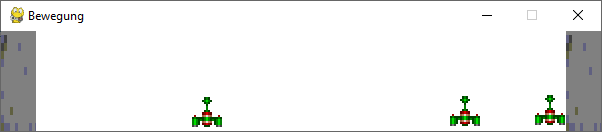
\includegraphics[scale=0.8]{invader06.png}};

\draw
 (-1.8cm,-1.3cm) node (a) {}
 (5.8cm,-1.3cm) node (b) {}
 (5.8cm,-0.57cm) node (c) {}
 (3.4cm,-0.57cm) node (d) {}
;
\draw[>->, very thick, red, densely dotted] (a) -- (b) ;
\draw[>->, very thick, red, densely dotted] (c) -- (d) ;

%node[above, black, xshift=-2.6cm] {move left}
%\draw[->] (a) -- (b);
%\draw[->] (o) -- (y);


%Left
%\draw
% (-0.15,3.4) node (left1) {}
% (3.15,3.4) node (left2) {}
%;
%
\end{tikzpicture}
\caption{Der Verteidiger bewegt sich und prallt ab}\label{picBewegung01}
\end{center}
\end{figure}


%%%%%%%%%%%%%%%%%%%%%%%%%%%%%%%%%%%%%%%%%%%%%%%%%%%%%%%%%%%%%%%%%%%%%%%%%%%%%%%%
\subsection*{Was war neu?}

\begin{itemize}
	\item Richtung und Geschwindigkeit in Variablen kodieren.

	\item Richtungswechsel durch Vorzeichenwechsel
	
	\item Kollisionserkennung kann durch Vergleich von Positionsangaben erfolgen.
	
	\item \texttt{blit()} verwendet ein \texttt{Rect}-Objekt.
	
	\item \texttt{pygame.Rect}:
	\myindex{pyg}{\texttt{Rect}}\\
	\url{https://www.pygame.org/docs/ref/rect.html}
	
	\item \texttt{pygame.Rect.move()}:
    \myindex{pyg}{\texttt{Rect}!\texttt{move()}}\\
    \url{https://www.pygame.org/docs/ref/rect.html#pygame.Rect.move}

	\item \texttt{pygame.Surface.get\_rect()}:
	\myindex{pyg}{\texttt{Surface}!\texttt{get\_rect()}}\\
	\url{https://www.pygame.org/docs/ref/surface.html#pygame.Surface.get_rect}

\end{itemize}


\newpage
\section{Sprite-Klasse}\index{Sprite}
%\subsection{Beispiel}
Im letzten Beispiel fiel auf, dass viele Variablen mit \texttt{defender\_} beginnen. Mit anderen Worten, es sind Attribute einer Sache und schreien förmlich nach einer Formulierung als Klasse. 

Diese Klasse soll alle Informationen bzgl. der Aktualisierung und Darstellung des Bitmaps enthalten. Einige Elemente wie \texttt{defender\_image} und \texttt{defender\_rect} scheinen aber doch bei jeder Bitmap-Verarbeitung eine Rolle zu spielen. Auch wird es bei jedem Bitmap einen Bedarf für Zustandsänderungen und für die Bildschirmausgabe geben. Tatsächlich gibt es in Pygame schon eine Klasse, die mir genau dazu ein \Gls{framework} bietet: \texttt{pygame.sprite.Sprite}\myindex{pyg}{\texttt{sprite}!\texttt{Sprite}|underline}\randnotiz{Sprite}. 

Formulieren wir also die Klasse \texttt{Defender} als eine Kindklasse von \texttt{Sprite} (\zeiref{srcInvader06a01}).

\lstsource{SRC/00 Einführung/05 Sprite/invader06a.py}{12}{37}{python}{Sprites (1), Version 1.0}{srcInvader06a1}

Die Zeilen des Konstruktors (\zeiref{srcInvader06a02}ff.) entsprechen denen der vorherigen Version. Lediglich der Präfix \texttt{defender\_} wird durch \texttt{self.} ersetzt, wodurch die Variablen zu Attributen der Klasse werden. Sie sollten keine Schwierigkeiten haben, diese zu verstehen.

Jede Kindklasse von \texttt{Sprite} muss zwei Attribute haben: \texttt{rect}\index{Sprite!self.rect|underline}\randnotiz{self.rect} und \texttt{image}\index{Sprite!self.image|underline}\randnotiz{self.image}. Auf diese beiden Attribute greifen nämlich die schon vorformulierten Lösungen zur Kollisionserkennung, Bildschirmausgabe etc. zu. Wir werden später noch den Nutzen sehen.

In \zeiref{srcInvader06a03}ff. werden die Randkollisionen und die Zustandsänderungen formuliert. Hier fällt besonders die Berechnung der neuen Position mit \texttt{move()}\myindex{pyg}{\texttt{rect}!\texttt{FRect}!\texttt{move()}} auf. 

Neu ist der Aufruf der Methode \texttt{change\_direction()}. Diese Methode (\zeiref{srcInvader06a08}) ist mehr \emph{OO-like} also die vorherige Version. In der objektorientierten Programmierung werden Algorithmen nicht direkt programmiert, sondern man sendet an das Objekt Nachrichten, und diese werden dann intern -- und von außen nicht sichtbar wie -- umgesetzt. Hier bedeutet dies, dass ich an der entsprechenden Stelle nicht den Richtungswechsel direkt durchführe, sondern mir selbst die Nachricht zusende, dass die Richtung geändert werden muss. 

Mit der Methode \texttt{draw()} in \zeiref{srcInvader06a04} wird die Bildschirmausgabe gekapselt.

\lstsource{SRC/00 Einführung/05 Sprite/invader06a.py}{40}{67}{python}{Sprites (2), Version 1.0}{srcInvader06a2}

Die Verwendung der Klasse \texttt{Defender} ist nun denkbar einfach geworden. In der \zeiref{srcInvader06a05} wird ein Objekt der Klasse erzeugt. In \zeiref{srcInvader06a06} wird \texttt{update()} aufgerufen und in \zeiref{srcInvader06a07} \texttt{draw()}.

Ein Vorteil der neuen Architektur ist die bessere Übersichtlichkeit und Verständlichkeit des Hauptprogrammes. Durch Namenskonvention (sprechende Klassen- und Funktionsnamen) wird der grundsätzliche Ablauf klarer und nicht mehr von Details überlagert.
%%%%%%%%%%%%%%%%%%%%%%%%%%%%%%%%%%


Ich möchte nun die Möglichkeiten der \texttt{Sprite}-Klasse nutzen, um die Kollisionsprüfung mit dem Rand nicht mehr selbst durchzuführen. 


Los geht's: Da wir die Kollisionsprüfung anders organisieren wollen, wird erstmal das \texttt{update()} wieder einfach. Wir berechnen lediglich die neue Position. 

Dabei wird in \zeiref{srcInvader06b01} die Methode \texttt{pygame.rect.FRect.move\_ip()}\myindex{pyg}{\texttt{rect}!\texttt{FRect}!\texttt{move\_ip()}|underline}\randnotiz{move\_ip()} eingeführt. Sie arbeitet wie \texttt{move()}, nur dass hier die Änderung direkt im Rechteck durchgeführt wird; \texttt{ip} steht hier für \emph{in place}. Bei \texttt{move()} bleibt das ursprüngliche Rechteck unverändert.


\lstsource{SRC/00 Einführung/05 Sprite/invader06b.py}{23}{24}{python}{Sprites (1), Version 1.1}{srcInvader06b1}

Damit die Ränder sichtbar werden und ich die Kollision besser erkennen kann, werden die Ränder nun zu zwei Steinwänden rechts und links; auch diese Bitmaps werden als Kindklasse von \texttt{pygame.sprite.Sprite} implementiert. Da der Zustand der beiden Wände sich nie verändert, kann ich auf die Programmierung von \texttt{update()} verzichten.

\lstsource{SRC/00 Einführung/05 Sprite/invader06b.py}{33}{44}{python}{Sprites (2), Version 1.1}{srcInvader06b2}

Nun erzeuge ich die beiden Ränder:

\lstsource{SRC/00 Einführung/05 Sprite/invader06b.py}{54}{55}{python}{Sprites (3), Version 1.1}{srcInvader06b3}

Bisher war alles easy. 

\lstsource{SRC/00 Einführung/05 Sprite/invader06b.py}{65}{70}{python}{Sprites (4), Version 1.1}{srcInvader06b4}

Was passiert hier? Mit der Methode \texttt{pygame.sprite.collide\_rect()}\myindex{pyg}{\texttt{sprite}!\texttt{collide\_rect()}}\randnotiz{collide\_rect()} werden die Rechtecke zweier \texttt{Sprite}-Objekte auf Kollision untersucht. Eine eigene Abfrage der linken und rechten Grenzen bleibt mir damit erspart.

Für beide Ränder -- allgemeiner gesprochen für viele \texttt{Sprite}-Objekte -- wird hier die Kollision mit einem einzelnen Objekt überprüft. Grundsätzlich kommen Sprites selten einzeln daher, sondern oft in Gruppen. Auch dies ist schon in Pygame vorgesehen und führt zu weiteren Vereinfachungen.

\lstsource{SRC/00 Einführung/05 Sprite/invader06c.py}{41}{75}{python}{Sprites (1), Version 1.2}{srcInvader06c1}

Der Verteidiger wird nicht mehr direkt angesprochen, sondern in eine Luxuskiste gepackt. Ich komme später nochmal darauf zurück. Die beiden \texttt{Border}-Objekte werden nicht mehr in zwei Objektvariablen abgelegt, sondern ebenfalls in eine Luxuskiste, der \texttt{pygame.sprite.Group}\myindex{pyg}{\texttt{sprite}!\texttt{Group}|underline}\randnotiz{Group}. Hier könnte ich nun noch andere Grenzen oder Grenzwälle ablegen. Von der Spiellogik her würden diese nun immer mit einem Schlag gemeinsam verarbeitet. Deutlich wird das bei diesem Minibeispiel an zwei Stellen.

Die erste Stelle ist \zeiref{srcInvader06c01} und dort wird eine andere Version der Kollisionsprüfung verwendet: \texttt{pygame.sprite.\-sprite\-collide()}\myindex{pyg}{\texttt{sprite}!\texttt{spritecollide()}|underline}\randnotiz{spritecollide()}. Der erste Parameter ist \emph{ein} \texttt{Sprite}-Objekt. In unserem Fall ist es der Verteidiger. Der zweite Parameter ist eine Spritegruppe mit allen \texttt{Border}-Objekten. Also wird der Verteidiger mit allen Mitgliedern der Gruppe auf Kollisionen überprüft. Dies funktioniert nur, wenn alle Sprites ein \texttt{Rect}- oder \texttt{FRect}-Objekt mit dem Namen \texttt{rect} als Attribut haben. Der dritte Parameter -- hier \false\ -- steuert, ob das kollidierende Sprite aus der Liste entfernt werden soll. Dieses Feature ist in Spielen recht interessant, will man doch beispielsweise Felsen, die von einem Raumschiff zerschossen wurden, löschen.

Die zweite Stelle ist \zeiref{srcInvader06c03}. Hier wird nicht mehr für jedes Objekt einzeln \texttt{draw()} aufgerufen, sondern für die ganze Gruppe. Nutzt man diesen Service, kann man die Methode \texttt{draw()} aus seiner eigenen Klasse (hier \texttt{Border} und \texttt{Defender}) entfernen, wodurch schon wieder alles einfacher wird.

Es scheint also eine gute Idee zu sein, die Sprites in solche Luxuskisten zu packen. Aber was war nochmal mit dem Defender? Um die Vorteile eine Spritegruppe nutzen zu können, kann man auch Gruppen anlegen, die nur ein Element enthalten. Damit diese Gruppen aber etwas effizienter arbeiten können -- schließlich weiß man ja, dass nur ein Element in der Gruppe ist --, gibt es dafür den Spezialfall \texttt{pygame.sprite.GroupSingle}\myindex{pyg}{\texttt{sprite}!\texttt{GroupSingle}|underline}\randnotiz{GroupSingle}. Da man oft den Bedarf hat, auf das einzige \texttt{Sprite}-Objekt der \emph{Gruppe} zuzugreifen, hat diese Gruppe das zusätzliche Attribut \texttt{sprite}\myindex{pyg}{\texttt{sprite}!\texttt{GroupSingle}!\texttt{sprite}} (siehe \zeiref{srcInvader06c01}f.).


Am Ende möchte ich meinen OO-Ansatz noch weiterverfolgen und auch das Hauptprogramm in eine \texttt{Game}-Klasse umwandeln. Wichtig ist mir dabei, gleich von Beginn an eine Strukturdisziplin zu etablieren. Je länger Sie in der Softwareentwicklung tätig bleiben, desto mehr freunden Sie sich mit Begriffen wie \emph{Ordnung} oder \emph{Struktur} an. Sie helfen auch bei komplexeren Spielen, nicht den roten Faden zu verlieren. Besonders hilfreich ist dabei das \Gls{srp}.

\newpage
\lstsource{SRC/00 Einführung/05 Sprite/invader06d.py}{41}{82}{python}{\texttt{Game}-Klasse}{srcInvader06d}

Ein Beispiel für den letzten Punkt ist die Einrichtung der Klasse \texttt{Game}. Hier wird der Quelltext nicht einfach ins \texttt{\_\_main\_\_}\index{\_\_main\_\_} gestellt, sondern gekapselt und geordnet und damit flexibel verfügbar gemacht. Ein Beispiel für das SRP sind die Methoden \texttt{watch\_for\_e\-vents()}, \texttt{update()} und \texttt{draw()}. Es ist eben nicht die Aufgabe von \texttt{run()} alles zu organisieren. Aus Sicht der Hauptprogrammschleife interessiert es mich nicht, welche Events abgefragt und wie sie verarbeitet werden. Ich will nur, dass die Events pro Frame einmal betrachet werden. Auch will sich \texttt{run()} nicht um die Reihenfolge kümmern, wie die Sprites auf den Bildschirm gezeichnet werden. Das soll die Methode \texttt{draw()} erledigen. Die Methode \texttt{run()} stellt nur sicher, dass zuerst die Sprites ihre neuen Zustände berechnen und dann die Ausgabe erfolgt.


Verbleibt noch ein Aspekt, den ich hier umsetzen möchte: Der Aufruf von \texttt{change\_di\-rec\-tion()} in \zeiref{srcInvader06d01} gefällt mir nicht. Er ist eine Verletzung von OO-Regeln. 

Die Spritegruppe ist eine Liste von \texttt{Sprite}-Objekten. Die Klasse \texttt{pygame.sprite.Sprite} kennt aber keine Methode \texttt{change\_direction()}. Deshalb ist das nicht ganz sauber, die hier aufzurufen. Python hat mit soetwas kein Problem, aber das sollte nicht der Maßstab sein. 

Es bietet sich vielmehr an, die Methode \texttt{update()} anzupassen. Schaut man sich die \gls{signatur} der Methode \texttt{pygame.sprite.Sprite.update()}\myindex{pyg}{\texttt{sprite}!\texttt{Sprite}!\texttt{update()}}\randnotiz{update()} genauer an, so sehen Sie, dass hier eigentlich frei definierbare Übergabeparameter vorgesehen sind.  Ich habe mir angewöhnt, einen Parameter mit Namen \texttt{action} zu benutzen, um Methoden der Kindklasse aufzurufen. So wird \texttt{change\_direction()} nach \zeiref{srcInvader06e02} durch \texttt{update()} aufgerufen und nicht mehr von außen.

\lstsource{SRC/00 Einführung/05 Sprite/invader06e.py}{24}{29}{python}{\texttt{Defender.update()}}{srcInvader06e1}

Der Aufruf erfolgt dann in \srcref[vref]{srcInvader06e2} in \zeiref{srcInvader06e03} indirekt durch die Verwendung des Übergabeparameters.

\lstsource{SRC/00 Einführung/05 Sprite/invader06e.py}{78}{81}{python}{\texttt{Game.update()}}{srcInvader06e2}

%%%%%%%%%%%%%%%%%%%%%%%%%%%%%%%%%%%%%%%%%%%%%%%%%%%%%%%%%%%%%%%%%%%%%%%%%%%%%%%%
\subsection*{Was war neu?}

Von der Verhaltenslogik her: \emph{gar nichts}. Die vorhandene Anwendung wurde nur in ein flexibles Framework eingebettet. 

Es wurden folgende Pygame-Elemente eingeführt:

\begin{itemize}
	\item \texttt{pygame.Rect.move()}:
	\myindex{pyg}{\texttt{Rect}!\texttt{move()}}\\
	\url{https://pyga.me/docs/ref/rect.html#pygame.Rect.move}

	\item \texttt{pygame.Rect.move\_ip()}:
	\myindex{pyg}{\texttt{Rect}!\texttt{move\_ip()}}\\
	\url{https://pyga.me/docs/ref/rect.html#pygame.Rect.move_ip}

	\item \texttt{pygame.sprite.Group}:
	\myindex{pyg}{\texttt{sprite}!\texttt{Group}}\\
	\url{https://pyga.me/docs/ref/sprite.html#pygame.sprite.Group}

	\item \texttt{pygame.sprite.GroupSingle}:
	\myindex{pyg}{\texttt{sprite}!\texttt{GroupSingle}}\\
	\url{https://pyga.me/docs/ref/sprite.html#pygame.sprite.GroupSingle}

	\item \texttt{pygame.sprite.GroupSingle.sprite}:
	\myindex{pyg}{\texttt{sprite}!\texttt{GroupSingle}!\texttt{sprite}}\\
\url{https://pyga.me/docs/ref/sprite.html#pygame.sprite.GroupSingle}

	\item \texttt{pygame.sprite.Sprite}:
	\myindex{pyg}{\texttt{sprite}!\texttt{Sprite}}\\
	\url{https://pyga.me/docs/ref/sprite.html#pygame.sprite.Sprite}
	
	\item \texttt{pygame.sprite.collide\_rect()}:
	\myindex{pyg}{\texttt{sprite}!\texttt{collide\_rect()}}\\
	\url{https://pyga.me/docs/ref/sprite.html#pygame.sprite.collide_rect}
	
	\item \texttt{pygame.sprite.spritecollide()}:
    \myindex{pyg}{\texttt{sprite}!\texttt{spritecollide()}}\\
    \url{https://pyga.me/docs/ref/sprite.html#pygame.sprite.spritecollide}
\end{itemize}



\newpage
%%%%%%%%%%%%%%%%%%%%%%%%%%%%%%%%%%%%%%%%%%%%%%%%%%%%%%%%%%%%%%%%%%%%%%%%%%%
\section{Tastatur}\index{Tastatur}
%\subsection{Beispiele}

\begin{wrapfigure}[10]{r}{3.1cm}%
	\begin{center}%
		\vspace{-1cm}%
		\myfigure{invader07.png}{0.8}{Ränder}{picInvader07}%
	\end{center}%
\end{wrapfigure}%
Ich möchte hier die Tastatur nicht erschöpfend behandeln, sondern lediglich das Grundprinzip verdeutlichen. So soll die Bewegungsrichtung durch die Pfeiltasten gesteuert werden können. Ebenso soll das Raumschiffe stehen bleiben oder sich wieder in Bewegung setzen können. Auch kann das Spiel jetzt durch die Escape-Taste verlassen werden (\Gls{boss}).

Zunächst bereiten wir die Verteidiger-Klasse vor bzw. wandeln sie ein wenig ab (\srcref[vref]{srcTastatur00a}). Das Sprite wird nun nicht mehr unten sondern mittig platziert (\zeiref{srcTastatur0001}). Das Raumschiff soll sich nun auch vertikal bewegen können. Dazu braucht es entweder zwei entsprechende Variablen oder aber ein \texttt{Vector2}-Objekt. Ich nehme ein \texttt{Vector2}-Objekt (\zeiref{srcTastatur0002}), wobei das erste Element der Richtungsvektor der horizontalen und das zweite der vertikalen Richtung ist. Der jeweilige Richtungsvektor wird dabei entsprechend der schon oben vorgestellten Semantik gesetzt. In der Methode \texttt{change\_direction()} werden nun beide Koordinaten berücksichtigt und aktualisiert. Bewegen und Stehenbleiben wird einfach dadurch erreicht, dass ich die Geschwindigkeit in \texttt{start()} auf~100 bzw. in \texttt{stop()} auf~0 setze.

\lstsource{SRC/00 Einführung/06 Tastatur/tastatur00.py}{18}{53}{python}{Bewegung durch Tastatur steuern (1), \texttt{Defender}}{srcTastatur00a} 

Die Klasse \texttt{Border} wird trivialerweise so erweitert, dass alle vier Seiten der Spielfläche nun durch eine Steinwand begrenzt werden (\srcref[vref]{srcTastatur00b}). Dazu wird im Konstruktor abgefragt, auf welcher Seite die Wand hochgezogen werden soll. Rechts und links wird das Bitmap in die Höhe gestreckt und oben und unten in die Breite. Anschließend wird das \texttt{Rect}-Objekt ermittelt und die Position festgelegt.

\lstsource{SRC/00 Einführung/06 Tastatur/tastatur00.py}{57}{77}{python}{Bewegung durch Tastatur steuern (2), \texttt{Border}}{srcTastatur00b}

Es werden dann die vier Objekte der \texttt{Border}-Klasse erzeugt und der Spritegruppe hinzugefügt.

\lstsource{SRC/00 Einführung/06 Tastatur/tastatur00.py}{88}{93}{python}{Bewegung durch Tastatur steuern (3), \texttt{Game}-Konstruktor}{srcTastatur00c}

Kommen wir jetzt zur eigentlichen Tastaturverarbeitung: Das Verwenden einer Taste kann die Ereignistypen \texttt{pygame.KEYDOWN}\myindex{pyg}{\texttt{KEYDOWN}|underline} oder \texttt{pygame.KEYUP}\myindex{pyg}{\texttt{KEYUP}|underline}\randnotiz{KEYDOWN\\KEYUP} auslösen. In unserem Beispiel (\zeiref{srcTastatur0003}) wollen wir wissen, welche Taste \emph{gedrückt} wurde, also verwenden wir \texttt{KEYDOWN}. Anschließend können wir über \texttt{pygame.event.key}\myindex{pyg}{\texttt{event}!\texttt{key}}\randnotiz{key} ermitteln, welche Taste gedrückt wurde. Dazu stellt uns Pygame in \texttt{pygame.key}\myindex{pyg}{\texttt{key}} eine Liste von vordefinierten Konstanten zur Verfügung (siehe \tabref[vref]{tabKey} und \tabref[vref]{tabKeyMod}).

\lstsource{SRC/00 Einführung/06 Tastatur/tastatur00.py}{109}{130}{python}{Bewegung durch Tastatur steuern (4), \texttt{Game}.\texttt{watch\_for\_events()}}{srcTastatur00d}

Fangen wir mit der Boss-Taste an. In \zeiref{srcTastatur0004} wird über die Konstante \texttt{K\_ESCAPE}\myindex{pyg}{\texttt{K\_ESCAPE}}\randnotiz{K\_ESCAPE} abgefragt, ob die gedrückte Taste die Escape-Taste ist. Wie beim Weg-Xen wird danach einfach das Flag der Hauptprogrammschleife auf \false\ gesetzt. Probieren Sie es aus!

Danach werden mit Hilfe von \randnotiz{K\_LEFT K\_RIGHT K\_UP K\_DOWN}\texttt{K\_LEFT}, \texttt{K\_RIGHT}, \texttt{K\_UP} und \texttt{K\_DOWN}\myindex{pyg}{\texttt{K\_LEFT}}\myindex{pyg}{\texttt{K\_RIGHT}}\myindex{pyg}{\texttt{K\_UP}}\myindex{pyg}{\texttt{K\_DOWN}} ab \zeiref{srcTastatur0005}ff. die vier Pfeiltasten abgefragt und die entsprechende Nachricht an den Verteidiger gesendet.

Mit Hilfe der Leerzeichen-Taste \texttt{K\_SPACE}\myindex{pyg}{\texttt{K\_SPACE}}\randnotiz{K\_SPACE} wird das Raumschiff in \zeiref{srcTastatur0006} gestoppt. 

Um den Einsatz der Shift-Taste (Umschalttaste) mal zu demonstrieren, habe ich hier das~\texttt{r} doppelt belegt (\zeiref{srcTastatur0007}). Das große~\texttt{R} stoppt das Raumschiff und das kleine~\texttt{r} startet es wieder. Dabei wird die Variable \texttt{event.mod}\myindex{pyg}{\texttt{event}!\texttt{mod}}\randnotiz{event.mod} mit Hilfe einer bitweisen Und-Verknüpfung dahingehend überprüft, ob das entsprechende Bit \texttt{KMOD\_LSHIFT}\myindex{pyg}{\texttt{KMOD\_LSHIFT}}\randnotiz{KMOD\_LSHIFT} für die linke Shift-Taste gedrückt wurde.

Dies soll ersteinmal ausreichen. Die Tastatur ist nur eine Möglichkeit der Spielsteuerung. Maus, Game-Controller oder Joystick sind ebenfalls in Pygame möglich.

\subsection*{Was war neu?}
Die Tastatur sendet Ereignisnachrichten, die man abfangen und auswerten kann. Dabei wird zum einen unterschieden, was mit der Tastatur gemacht wurde (\texttt{event.typ}) und dann mit welcher Taste (\texttt{event.key}). Über \texttt{event.mod} kann bitweise abgefragt werden, welche Steuertasten auf der Tastatur verwendet wurden.

Es wurden folgende Pygame-Elemente eingeführt:


\begin{itemize}
	\item \texttt{pygame.key}:
	\myindex{pyg}{\texttt{KEY}|underline}\\ \url{https://www.pygame.org/docs/ref/key.html}

	\item \texttt{pygame.KEYDOWN}, \texttt{pygame.KEYUP}:
	\myindex{pyg}{\texttt{KEYDOWN}}\myindex{pyg}{\texttt{KEYUP}}\\ \url{https://www.pygame.org/docs/ref/event.html}
	
\end{itemize}

\begin{longtable}{lll}
	\caption{Liste von vordefinierten Tastaturkonstanten}\label{tabKey} \\
	% Definition des Tabellenkopfes auf der ersten Seite
     Konstante & Bedeutung & Beschreibung \\\hline\hline
	\hline
	\endfirsthead % Erster Kopf zu Ende
	% Definition des Tabellenkopfes auf den folgenden Seiten
	\caption{Liste von vordefinierten Tastaturkonstanten (Fortsetzung)}\\
	 Konstante & Bedeutung & Beschreibung \\\hline\hline
	\hline
	\endhead % Zweiter Kopf ist zu Ende
	% Ab hier kommt der Inhalt der Tabelle
\texttt{K\_BACKSPACE}    &  \verb+\b+    &  Löschen (backspace) \\ \hline
\texttt{K\_TAB}          &  \verb+\t+    &  Tabulator\\ \hline
\texttt{K\_CLEAR}        &  \verb++      &  Leeren\\ \hline
\texttt{K\_RETURN}       &  \verb+\r+    &  Eingabe (return, enter)\\ \hline
\texttt{K\_PAUSE}        &  \verb++      &  Pause\\ \hline
\texttt{K\_ESCAPE}       &  \verb+^[+    &  Abbruch (escape)\\ \hline
\texttt{K\_SPACE}        &  \verb+ +     &  Leerzeichen (space)\\ \hline
\texttt{K\_EXCLAIM}      &  \verb+!+     &  Ausrufezeichen\\ \hline
\texttt{K\_QUOTEDBL}     &  \verb+"+     &  Gänsefüßchen\\ \hline
\texttt{K\_HASH}         &  \verb+#+     &  Doppelkreuz (hash)\\ \hline
\texttt{K\_DOLLAR}       &  \verb+$+     &  Dollar\\ \hline
\texttt{K\_AMPERSAND}    &  \verb+&+     &  Kaufmannsund\\ \hline
\texttt{K\_QUOTE}        &  \verb+'+     &  Hochkomma\\ \hline
\texttt{K\_LEFTPAREN}    &  \verb+(+     &  Linke runde Klammer\\ \hline
\texttt{K\_RIGHTPAREN}   &  \verb+)+     &  Rechte runde Klammer\\ \hline
\texttt{K\_ASTERISK}     &  \verb+*+     &  Sternchen\\ \hline
\texttt{K\_PLUS}         &  \verb-+-     &  Plus\\ \hline
\texttt{K\_COMMA}        &  \verb+,+     &  Komma\\ \hline
\texttt{K\_MINUS}        &  \verb+-+     &  Minus\\ \hline
\texttt{K\_PERIOD}       &  \verb+.+     &  Punkt\\ \hline
\texttt{K\_SLASH}        &  \verb+/+     &  Schrägstrich\\ \hline
\texttt{K\_0}            &  \verb+0+     &  0\\ \hline
\texttt{K\_1}            &  \verb+1+     &  1\\ \hline
\texttt{K\_2}            &  \verb+2+     &  2\\ \hline
\texttt{K\_3}            &  \verb+3+     &  3\\ \hline
\texttt{K\_4}            &  \verb+4+     &  4\\ \hline
\texttt{K\_5}            &  \verb+5+     &  5\\ \hline
\texttt{K\_6}            &  \verb+6+     &  6\\ \hline
\texttt{K\_7}            &  \verb+7+     &  7\\ \hline
\texttt{K\_8}            &  \verb+8+     &  8\\ \hline
\texttt{K\_9}            &  \verb+9+     &  9\\ \hline
\texttt{K\_COLON}        &  \verb+:+     &  Doppelpunkt\\ \hline
\texttt{K\_SEMICOLON}    &  \verb+;+     &  Semicolon\\ \hline
\texttt{K\_LESS}         &  \verb+<+     &  Kleiner\\ \hline
\texttt{K\_EQUALS}       &  \verb+=+     &  Gleich\\ \hline
\texttt{K\_GREATER}      &  \verb+>+     &  Größer\\ \hline
\texttt{K\_QUESTION}     &  \verb+?+     &  Fragezeichen\\ \hline
\texttt{K\_AT}           &  \makeatletter \verb+@+ \makeatother    &  Klammeraffe\\ \hline
\texttt{K\_LEFTBRACKET}  &  \verb+[+     &  Linke eckige Klammer\\ \hline
\texttt{K\_BACKSLASH}    &  \verb+\+     &  Umgekehrter Schrägstrich\\ \hline
\texttt{K\_RIGHTBRACKET} &  \verb+]+     &  Rechte eckige Klammer\\ \hline
\texttt{K\_CARET}        &  \verb+^+     &  Hütchen\\ \hline
\texttt{K\_UNDERSCORE}   &  \verb+_+     &  Unterstrich\\ \hline
\texttt{K\_BACKQUOTE}    &  \verb+`+     &  Akzent Grvis\\ \hline
\texttt{K\_a}            &  \verb+a+     &  a\\ \hline
\texttt{K\_b}            &  \verb+b+     &  b\\ \hline
\texttt{K\_c}            &  \verb+c+     &  c\\ \hline
\texttt{K\_d}            &  \verb+d+     &  d\\ \hline
\texttt{K\_e}            &  \verb+e+     &  e\\ \hline
\texttt{K\_f}            &  \verb+f+     &  f\\ \hline
\texttt{K\_g}            &  \verb+g+     &  g\\ \hline
\texttt{K\_h}            &  \verb+h+     &  h\\ \hline
\texttt{K\_i}            &  \verb+i+     &  i\\ \hline
\texttt{K\_j}            &  \verb+j+     &  j\\ \hline
\texttt{K\_k}            &  \verb+k+     &  k\\ \hline
\texttt{K\_l}            &  \verb+l+     &  l\\ \hline
\texttt{K\_m}            &  \verb+m+     &  m\\ \hline
\texttt{K\_n}            &  \verb+n+     &  n\\ \hline
\texttt{K\_o}            &  \verb+o+     &  o\\ \hline
\texttt{K\_p}            &  \verb+p+     &  p\\ \hline
\texttt{K\_q}            &  \verb+q+     &  q\\ \hline
\texttt{K\_r}            &  \verb+r+     &  r\\ \hline
\texttt{K\_s}            &  \verb+s+     &  s\\ \hline
\texttt{K\_t}            &  \verb+t+     &  t\\ \hline
\texttt{K\_u}            &  \verb+u+     &  u\\ \hline
\texttt{K\_v}            &  \verb+v+     &  v\\ \hline
\texttt{K\_w}            &  \verb+w+     &  w\\ \hline
\texttt{K\_x}            &  \verb+x+     &  x\\ \hline
\texttt{K\_y}            &  \verb+y+     &  y\\ \hline
\texttt{K\_z}            &  \verb+z+     &  z\\ \hline
\texttt{K\_DELETE}       &  \verb+ +     &  Löschen (delete)\\ \hline
\texttt{K\_KP0}          &  \verb+ +     &  Nummernfeld 0\\ \hline
\texttt{K\_KP1}          &  \verb+ +     &  Nummernfeld 1\\ \hline
\texttt{K\_KP2}          &  \verb+ +     &  Nummernfeld 2\\ \hline
\texttt{K\_KP3}          &  \verb+ +     &  Nummernfeld 3\\ \hline
\texttt{K\_KP4}          &  \verb+ +     &  Nummernfeld 4\\ \hline
\texttt{K\_KP5}          &  \verb+ +     &  Nummernfeld 5\\ \hline
\texttt{K\_KP6}          &  \verb+ +     &  Nummernfeld 6\\ \hline
\texttt{K\_KP7}          &  \verb+ +     &  Nummernfeld 7\\ \hline
\texttt{K\_KP8}          &  \verb+ +     &  Nummernfeld 8\\ \hline
\texttt{K\_KP9}          &  \verb+ +     &  Nummernfeld 9\\ \hline
\texttt{K\_KP\_PERIOD}   &  \verb+.+     &  Nummernfeld Punkt\\ \hline
\texttt{K\_KP\_DIVIDE}   &  \verb+/+     &  Nummernfeld Geteilt/Schrägstrich\\ \hline
\texttt{K\_KP\_MULTIPLY} &  \verb+*+     &  Nummernfeld Mal/Sternchen\\ \hline
\texttt{K\_KP\_MINUS}    &  \verb+-+     &  Nummernfeld Minus\\ \hline
\texttt{K\_KP\_PLUS}     &  \verb-+-     &  Nummernfeld Plus\\ \hline
\texttt{K\_KP\_ENTER}    &  \verb+\r+    &  Nummernfeld Eingabe (return, enter)\\ \hline
\texttt{K\_KP\_EQUALS}   &  \verb+=+     &  Nummernfeld Gleich\\ \hline
\texttt{K\_UP}           &  \verb+ +     &  Pfeil nach oben\\ \hline
\texttt{K\_DOWN}         &  \verb+ +     &  Pfeil nach unten\\ \hline
\texttt{K\_RIGHT}        &  \verb+ +     &  Pfeil nach rechts\\ \hline
\texttt{K\_LEFT}         &  \verb+ +     &  Pfeil nach links\\ \hline
\texttt{K\_INSERT}       &  \verb+ +     &  Einfügen ein/aus\\ \hline
\texttt{K\_HOME}         &  \verb+ +     &  Pos1\\ \hline
\texttt{K\_END}          &  \verb+ +     &  Ende\\ \hline
\texttt{K\_PAGEUP}       &  \verb+ +     &  Hochblättern\\ \hline
\texttt{K\_PAGEDOWN}     &  \verb+ +     &  Runterblättern\\ \hline
\texttt{K\_F1}           &  \verb+ +     &  F1\\ \hline
\texttt{K\_F2}           &  \verb+ +     &  F2\\ \hline
\texttt{K\_F3}           &  \verb+ +     &  F3\\ \hline
\texttt{K\_F4}           &  \verb+ +     &  F4\\ \hline
\texttt{K\_F5}           &  \verb+ +     &  F5\\ \hline
\texttt{K\_F6}           &  \verb+ +     &  F6\\ \hline
\texttt{K\_F7}           &  \verb+ +     &  F7\\ \hline
\texttt{K\_F8}           &  \verb+ +     &  F8\\ \hline
\texttt{K\_F9}           &  \verb+ +     &  F9\\ \hline
\texttt{K\_F10}          &  \verb+ +     &  F10\\ \hline
\texttt{K\_F11}          &  \verb+ +     &  F11\\ \hline
\texttt{K\_F12}          &  \verb+ +     &  F12\\ \hline
\texttt{K\_F13}          &  \verb+ +     &  F13\\ \hline
\texttt{K\_F14}          &  \verb+ +     &  F14\\ \hline
\texttt{K\_F15}          &  \verb+ +     &  F15\\ \hline
\texttt{K\_NUMLOCK}      &  \verb+ +     &  Umschalten Zahlen\\ \hline
\texttt{K\_CAPSLOCK}     &  \verb+ +     &  Umschalten Großbuchstaben\\ \hline
\texttt{K\_SCROLLOCK}    &  \verb+ +     &  Umschalten auf scrollen\\ \hline
\texttt{K\_RSHIFT}       &  \verb+ +     &  Rechte Umschalttaste\\ \hline
\texttt{K\_LSHIFT}       &  \verb+ +     &  Linke Umschalttaste\\ \hline
\texttt{K\_RCTRL}        &  \verb+ +     &  Rechte Steuerungstaste\\ \hline
\texttt{K\_LCTRL}        &  \verb+ +     &  Linke Steuerungstaste\\ \hline
\texttt{K\_RALT}         &  \verb+ +     &  Rechte Alterntivtaste\\ \hline
\texttt{K\_LALT}         &  \verb+ +     &  Linke Alternativtaste\\ \hline
\texttt{K\_RMETA}        &  \verb+ +     &  Rechte Metataste\\ \hline
\texttt{K\_LMETA}        &  \verb+ +     &  Linke Metataste\\ \hline
\texttt{K\_LSUPER}       &  \verb+ +     &  Linke Windowstaste\\ \hline
\texttt{K\_RSUPER}       &  \verb+ +     &  Rechte Windowstaste\\ \hline
\texttt{K\_MODE}         &  \verb+ +     &  AltGr Umschalter\\ \hline
\texttt{K\_HELP}         &  \verb+ +     &  Hilfe\\ \hline
\texttt{K\_PRINT}        &  \verb+ +     &  Bildschirmdruck/Screenshot\\ \hline
\texttt{K\_SYSREQ}       &  \verb+ +     &  Systemabfrage\\ \hline
\texttt{K\_BREAK}        &  \verb+ +     &  Abbruch/Unterbrechung\\ \hline
\texttt{K\_MENU}         &  \verb+ +     &  Menü\\ \hline
\texttt{K\_POWER}        &  \verb+ +     &  Ein-/Ausschalten\\ \hline
\texttt{K\_EURO}         &  \verb+€+     &  Euro-Währungszeichen\\ \hline
\texttt{K\_AC\_BACK}     &  \verb+ +     &  Android Zurückschalter\\ \hline
\end{longtable} 

\begin{longtable}{ll}
	\caption{Liste von vordefinierten Konstanten zur Tastaturschaltung}\label{tabKeyMod} \\
	% Definition des Tabellenkopfes auf der ersten Seite
	Konstante  & Beschreibung \\\hline\hline
	\hline
	\endfirsthead % Erster Kopf zu Ende
	% Definition des Tabellenkopfes auf den folgenden Seiten
	\caption{Liste von vordefinierten Konstanten zur Tastaturschaltung (Fortsetzung)}\\
	Konstante & Beschreibung \\\hline\hline
	\hline
	\endhead % Zweiter Kopf ist zu Ende
	% Ab hier kommt der Inhalt der Tabelle
    \texttt{KMOD\_NONE}   &  Keine Belegungstaste gedrückt\\ \hline
    \texttt{KMOD\_LSHIFT} &  Linke Umschalttaste\\ \hline
    \texttt{KMOD\_RSHIFT} &  Rechte Umschalttaste\\ \hline
    \texttt{KMOD\_SHIFT}  &  Linke oder rechte Umschalttaste oder beide\\ \hline
    \texttt{KMOD\_LCTRL}  &  Linke Steuerungstaste\\ \hline
    \texttt{KMOD\_RCTRL}  &  Rechte Steuerungstaste\\ \hline
    \texttt{KMOD\_CTRL}   &  Linke oder rechte Steuerungstaste oder beide\\ \hline
    \texttt{KMOD\_LALT}   &  Linke Alternativtaste\\ \hline
    \texttt{KMOD\_RALT}   &  Rechte Alternativtaste\\ \hline
    \texttt{KMOD\_ALT}    &  Linke oder rechte Alternativtaste oder beide\\ \hline
    \texttt{KMOD\_LMETA}  &  Linke Metataste\\ \hline
    \texttt{KMOD\_RMETA}  &  Rechte Metataste\\ \hline
    \texttt{KMOD\_META}   &  Linke oder rechte Metataste oder beide\\ \hline
    \texttt{KMOD\_CAPS}   &  Umschalten Großbuchstaben\\ \hline
    \texttt{KMOD\_NUM}    &  Umschalten Zahlen\\ \hline
    \texttt{KMOD\_MODE}   &  AltGr Umschalter\\ \hline
\end{longtable} 


\newpage
%%%%%%%%%%%%%%%%%%%%%%%%%%%%%%%%%%%%%%%%%%%%%%%%%%%%%%%%%%%%%%%%%%%%%%%%%%%
\section{Textausgabe mit Fonts}\index{Font}
\subsection{Default-Font}
\myebild{font01}{0.8}{Textausgabe mit Fonts}{picFont01}

Bei vielen Spielen werden Informationen nicht nur symbolisch auf die Spielfläche gebracht (z.B. drei Männchen für drei Leben), sondern auch in Schriftform. Eine Möglichkeit dies zu erreichen, ist die Textausgabe mit Hilfe installierter Fonts. Dabei wird zuerst ein \texttt{Font}-Objekt erstellt und durch ihn ein \texttt{Surface}-Objekt mit dem Text erzeugt (\glslink{render}{gerendert)}\index{Rendern}\randnotiz{Rendern}. Ich habe dies für ein kleines Beispiel in eine Klasse gekapselt, die Sie ja nach Belieben aufbohren oder anpassen können.

Zuerst importieren wir ein paar Konstanten. Die Klasse \texttt{Settings} überspringe ich mal, die hat sich nicht verändert:

\lstsource{SRC/00 Einführung/07 Fonts/textoutput_simple.py}{1}{5}{python}{Text mit Fonts ausgeben (1), Präambel}{srcFonts00a} 

Und nun die Klasse \texttt{TextSprite}: Lassen Sie sich nicht vom \glslink{oo}{OO}-Ansatz verwirren. Eigentlich ist alles ganz einfach. Wir brauchen ein \texttt{pygame.font.\-Font}-Objekt\myindex{pyg}{\texttt{font}!\texttt{Font}}\randnotiz{Font}. Dieses wiederum braucht zwei Infos: Welchen installierten \Gls{font} es benutzen soll, und die Fontgröße in \glslink{pt}{$pt$}. Eine Möglichkeit zu einem installierten Font zu kommen, ist die Methode \texttt{pygame.font.get\_default\_font()}\myindex{pyg}{\texttt{font}!\texttt{get\_default\_font()}}\randnotiz{get\_default\_font()}. Ihr Aufruf in \zeiref{srcTextoutputSimple01} liefert mir die vom Betriebssystem eingestellte Zeichsatzvorgabe. Die Schriftgröße (\texttt{fontsize}) legen wir nach Bedarf einfach fest. 

\lstsource{SRC/00 Einführung/07 Fonts/textoutput_simple.py}{16}{43}{python}{Text mit Fonts ausgeben (2), \texttt{TextSprite}}{srcFonts00b} 

Schauen wir uns nun den Konstruktor etwas genauer an. Die  Attribute \texttt{image} und \texttt{rect} werden hier einfach schonmal als Dummies angelegt; könnte man auch lassen. Nachdem ich die übergebenen Informationen über Textgröße und -farbe in Attribute abgespeichert habe, kann ich das \texttt{Font}-Objekt erstellen lassen. Dies erfolgt durch den Aufruf von \texttt{fontsize\_update()} in \zeiref{srcTextoutputSimple02}. Durch die Angabe~0 wird klar, dass hier nicht die Größe verändert werden soll, sondern nur, dass die Objekterzeugung passiert. 

Nun merke ich mir den eigentlichen Text, der zu einem Schriftzug gerendert werden soll und, wo das das Zentrum des Schriftzug platziert wird. Jetzt habe ich alle Infos zusammen und kann durch Aufruf von \texttt{render()} in \zeiref{srcTextoutputSimple03} mit Hilfe von \texttt{pygame\-.font\-.ren\-der()}\myindex{pyg}{\texttt{font}!\texttt{Font}!\texttt{render()}}\randnotiz{render()} das \texttt{Surface}-Objekt erzeugen (\zeiref{srcTextoutputSimple04}). Anschließend wird vom Bitmap das Rechteck ermittelt und das Zentrum des Rechtecks auf die gewünschte Position verschoben.

Jetzt noch die zwei Methoden \texttt{fontsize\_update()} und \texttt{fontcolor\_update()}: Beide ermöglichen es mir, zur Laufzeit die Schriftgröße und -farbe zu ändern. Die Semantik sollte selbsterklärend sein.

Wie kann man nun so eine Klasse nutzen? Hier ein Beispiel. In der Mitte soll ein Gruß erscheinen. Dazu verwende ich das Objekt \texttt{hello} (\zeiref{srcTextoutputSimple07}). Darunter soll durch \texttt{info} ausgegeben werden, mit welcher Schriftgröße und -farbe der Gruß erzeugt wurde (\zeiref{srcTextoutputSimple07}). 

\newpage
\lstsource{SRC/00 Einführung/07 Fonts/textoutput_simple.py}{47}{94}{python}{Text mit Fonts ausgeben (3),  Hauptprogramm}{srcFonts00c} 

Dieser Gruß kann durch die Plus- und Minus-Tasten in seiner Größe verändert werden (\zeiref{srcTextoutputSimple05}ff.). Die Tasten \texttt{r}, \texttt{g} und \texttt{b} werden dazu verwendet, den jeweiligen Farbkanal zu manipulieren. Der Großbuchstabe erhöht den Wert (z.B. in \zeiref{srcTextoutputSimple09}), der Kleinbuchstabe reduziert ihn (z.B. in \zeiref{srcTextoutputSimple10}).

In \abbref[vref]{picFont01} können Sie eine mögliche Darstellung sehen.

\subsection{Fontliste}

\myebild{font02}{0.8}{Fontliste}{picFont02}

Als weiteres Beispiel möchte ich Ihnen ein kleines Programm zeigen, welches alle installierten Fonts auflistet. Vielleicht kann man sich ja dabei Gestaltungsideen holen. Der erste Teil sollte keine Verständnisprobleme mehr bereiten.

\lstsource{SRC/00 Einführung/07 Fonts/textoutput_fontslist.py}{1}{40}{python}{Fontliste (1), \texttt{Präambel}, \texttt{Settings} und \texttt{Textsprite}}{srcFonts01a} 

Die Klasse \texttt{TextSprite} wurde nur wenig auf die Bedürfnisse angepasst. Die Klasse \texttt{BigImage} hat nur die Aufgabe, alle \texttt{FontSprite}-Images als großes Bild zu verwalteten. Später wird immer ein Ausschnitt aus dem Bitmap auf den Bildschirm gedruckt. Der Ausschnitt orientiert sich an der Position innerhalb der Liste und wird durch das Attribut \texttt{offset} gesteuert und in der Methode \texttt{update()} (\zeiref{srcTextoutputFontlist01}) ermittelt. Zuerst wird ermittelt, ob ich das obere oder untere Ende des Bitmaps erreicht habe. Falls ja, wird \texttt{top} bzw. \texttt{bottom} entsprechnd gesetzt, so dass immer der ganze Bildschirm gefüllt wird. Ansonsten wird das \texttt{offset}-Rechteck nach oben bzw. nach unten verschoben und mit \texttt{pygame.Surface.subsurface()}\myindex{pyg}{\texttt{Surface}!\texttt{subsurface()}}\randnotiz{subsurface()} der Ausschnitt ermittelt.

\lstsource{SRC/00 Einführung/07 Fonts/textoutput_fontslist.py}{43}{62}{python}{Fontliste (2), \texttt{BigImage}}{srcFonts01b} 

Und jetzt das Hauptprogramm. Im ersten Teil wird über \texttt{pygame.font.get\_fonts()}\myindex{pyg}{\texttt{font}!\texttt{get\_fonts()}}\randnotiz{get\_fonts()} (\zeiref{srcTextoutputFontlist02}) eine Liste aller installierten Fontnamen ermittelt. Dieser Name wird dem Konstruktor von \texttt{TestSprite} übergeben. Mit Hilfe der Methode \texttt{pygame.font.match\_font()}\myindex{pyg}{\texttt{font}!\texttt{match\_font()}}\randnotiz{match\_font()} (\zeiref{srcTextoutputFontlist03})wird nun der Font selbst im System gesucht, wobei sich diese Methode zunutze macht, dass der Name der Fontdatei sich aus dem Fontnamen und der Endung~\glslink{ttf}{\texttt{ttf}} herleiten lässt.

\newpage
\lstsource{SRC/00 Einführung/07 Fonts/textoutput_fontslist.py}{67}{112}{python}{Fontliste (3), Hauptprogramm (1)}{srcFonts01c} 

In der \forSchleife\_ werden nun für alle Fonts \texttt{TextSprite}-Objekte erzeugt und deren Höhe und Breite ermittelt. Diese vielen Bitmaps werden dann auf das große Bitmap gedruckt (\zeiref{srcTextoutputFontlist04}).

\lstsource{SRC/00 Einführung/07 Fonts/textoutput_fontslist.py}{97}{999}{python}{Fontliste, Hauptprogramm (2)}{srcFonts01d} 

Die Hauptprogrammschleife übernimmt nun nur noch das Blättern (jeweils um eine drittel Bildschirmhöhe) und das Programmende.

\subsection*{Was war neu?}

Es wurden folgende Pygame-Elemente eingeführt:

\begin{itemize}
	\item \texttt{pygame.font.Font}:
	\myindex{pyg}{\texttt{font}!\texttt{Font}}\\ \url{https://www.pygame.org/docs/ref/font.html}
	
	\item \texttt{pygame.font.get\_default\_font()}:
	\myindex{pyg}{\texttt{font}!\texttt{get\_default\_font()}}\\ \url{https://www.pygame.org/docs/ref/font.html#pygame.font.get_default_font}

	\item \texttt{pygame.font.get\_fonts()}:
	\myindex{pyg}{\texttt{font}!\texttt{get\_fonts()}}\\ \url{https://www.pygame.org/docs/ref/font.html#pygame.font.get_fonts}
	
    \item \texttt{pygame.font.match\_font()}:
    \myindex{pyg}{\texttt{font}!\texttt{match\_font()}}\\
    \url{https://www.pygame.org/docs/ref/font.html#pygame.font.match_font}

	\item \texttt{pygame.font.Font.render()}:
    \myindex{pyg}{\texttt{font}!\texttt{Font}!\texttt{render()}}\\ \url{https://www.pygame.org/docs/ref/font.html#pygame.font.Font.render}

	\texttt{pygame.Surface.subsurface()}:
    \myindex{pyg}{\texttt{Surface}!\texttt{subsurface()}}\\ \url{https://www.pygame.org/docs/ref/surface.html#pygame.Surface.subsurface}


\end{itemize}

\input{0108_Textbitmaps.tex}
%%%%%%%%%%%%%%%%%%%%%%%%%%%%%%%%%%%%%%%%%%%%%%%%%%%%%%%%%%%%%%%%%%%%%%%%%%%
\section{Kollisionserkennung}\index{Kollision}
%\subsection{Beispiele}
Kollisionserkennung wird in der Spieleprogrammierung  oft gebraucht: Personen können nicht durch Hindernisse gehen, Geschosse treffen auf Ziele, Bälle prallen ab usw.. Deshalb stellt Pygame einen ganzen Blumenstrauß von Kollisionserkennungen zur Verfügung:

\begin{itemize}
    \item \textbf{Rechtecküberschneidung}\index{Kollisionserkennung!Rechteck}: Wir haben schon bei Betrachtung der \texttt{Sprite}-Klasse gesehen, dass das Attribut \texttt{rect} notwendig ist. Dieses enthält die Positions- und Größenangaben des umgebenen Rechtecks. Treffen nun zwei Sprites aufeinander, wird überprüft, ob sich die beiden Rechtecke überschneiden. Dies ist eine sehr \emph{billige} Erkennungsmethode, da mit wenigen Vergleichen entschieden werden kann, ob sich zwei Rechtecke treffen/überlappen. Hier eine beispielhafte Programmierung:
\lstset{firstnumber=1}
\begin{lstlisting}
def rectangleCollision(rect1, rect2):
    return rect1.left < rect2.right and
           rect2.left < rect1.right and
           rect1.top < rect2.bottom and
           rect2.top < rect1.bottom
\end{lstlisting}


\begin{figure}[H]
\begin{center}
\tikzset{
    shape rechteck/.style= {
    draw,
    line width = 1pt,
    inner xsep = 0.0cm,
    inner ysep = 0.0cm,
   }
}

\begin{tikzpicture}
\tiny
\draw [->, name=xachse] (0cm, 6cm)  -- +(13cm, 0cm);
\draw [<-, name=yachse] (0cm, 0cm)  -- +(0cm, 6cm);

\pgfsetfillopacity{0.5}
\draw (4.0cm, 3.0cm) node[name=k1,shape=rectangle,shape rechteck, fill = yellow!30, minimum height = 4.0cm, minimum width = 3cm] {};
\draw (6.5cm, 2.0cm) node[name=k2,shape=rectangle,shape rechteck, fill = green!30, minimum height = 3.5cm, minimum width = 5cm] {};
\pgfsetfillopacity{1.0}

\draw[-, very thick, red, dotted]  let \p1 = (k1.north west) in (k1.north west) --  (\x1, 6.0cm);
\draw[-, very thick, red, dotted]  let \p1 = (k1.north west) in (k1.north west) --  (0cm, \y1);
\draw[-, very thick, blue, dotted] let \p1 = (k1.north east) in (k1.north east) --  (\x1, 6.0cm);
\draw[-, very thick, blue, dotted] let \p1 = (k1.south west) in (k1.south west) --  (0cm,\y1);

\draw[-, very thick, red, dotted]  let \p1 = (k2.north west) in (k2.north west) --  (\x1, 6.0cm);
\draw[-, very thick, red, dotted]  let \p1 = (k2.north west) in (k2.north west) --  (0cm, \y1);
\draw[-, very thick, blue, dotted] let \p1 = (k2.north east) in (k2.north east) --  (\x1, 6.0cm);
\draw[-, very thick, blue, dotted] let \p1 = (k2.south west) in (k2.south west) --  (0cm,\y1);

\path [name=x1, color=red] let \p1 = (k1.north west) in node  at (\x1,6.4cm) {$left_1$};
\path [name=x2, color=red] let \p1 = (k2.north west) in node  at (\x1,6.4cm) {$left_2$};
\path [name=x1, color=blue] let \p1 = (k1.north east) in node  at (\x1,6.4cm) {$right_1$};
\path [name=x2, color=blue] let \p1 = (k2.north east) in node  at (\x1,6.4cm) {$right_2$};
\path [name=y1, color=red] let \p1 = (k1.north west) in node  at (-0.5cm,\y1) {$top_1$};
\path [name=y2, color=red] let \p1 = (k2.north west) in node  at (-0.5cm,\y1) {$top_2$};
\path [name=y1, color=blue] let \p1 = (k1.south west) in node  at (-0.9cm,\y1) {$bottom_1$};
\path [name=y2, color=blue] let \p1 = (k2.south west) in node  at (-0.9cm,\y1) {$bottom_2$};
\end{tikzpicture}
\caption{Kollisionserkennung mit Rechtecken}\label{picKollRect01}
\end{center}
\end{figure}



    \item \textbf{Kreisüberschneidung}\index{Kollisionserkennung!Kreis}: Bei eher runden Sprites empfiehlt es sich, nicht die Rechtecke zu überprüfen, sondern den Innenkreis zur Kollisionsprüfung zu verwenden. Auch diese Kollisionsprüfung ist recht schnell, da nur ein Vergleich auf den Abstand der Mittelpunkte erfolgen muss: $\sqrt{(x_2-x_1)^2+(y_2-y_1)^2} < r_1+r_2$.

\begin{figure}[H]
\begin{center}
\tikzset{
    shape kreis/.style= {
    draw,
    fill = yellow!30,
    line width = 1pt,
    inner xsep = 0.0cm,
    inner ysep = 0.0cm,
   }
}

\begin{tikzpicture}
\draw [->, name=xachse] (0cm, 0cm)  -- +(13cm, 0cm);
\draw [->, name=yachse] (0cm, 0cm)  -- +(0cm, 6cm);

\draw (4.0cm, 3.5cm) node[name=k1,shape=circle,shape kreis,  minimum height = 4cm] {};
\draw (8.5cm, 2.5cm) node[name=k2,shape=circle,shape kreis,  minimum height = 3cm] {};

\draw[-, very thick, blue] 
 (k1.north west) --  node[above, blue, xshift=0cm] {$r_1$} (k1.center);
\draw[-, very thick, blue] 
 (k2.north east) --  node[above, blue, xshift=0cm] {$r_2$} (k2.center);

\draw[-, very thick, blue] 
 (k1.center) --  node[above, blue, sloped, xshift=0cm] {\footnotesize$\sqrt{(x_2-x_1)^2+(y_2-y_1)^2}$} (k2.center);

\draw[-, very thick, red, dotted] 
 (k1.center) --  +(0cm, -3.5cm);
\draw[-, very thick, red, dotted] 
 (k1.center) --  +(-4.0cm, 0cm);

\draw[-, very thick, red, dotted] 
 (k2.center) --  +(0cm, -2.5cm);
\draw[-, very thick, red, dotted] 
 (k2.center) --  +(-8.5cm, 0cm);

\path [name=x1, color=red] let \p1 = (k1) in node  at (\x1,-0.4cm) {$x_1$};
\path [name=x2, color=red] let \p1 = (k2) in node  at (\x1,-0.4cm) {$x_2$};
\path [name=y1, color=red] let \p1 = (k1) in node  at (-0.4cm,\y1) {$y_1$};
\path [name=y2, color=red] let \p1 = (k2) in node  at (-0.4cm,\y1) {$y_2$};
\end{tikzpicture}
\caption{Kollisionserkennung mit Kreisen}\label{picKollKreis01}
\end{center}
\end{figure}

    \item \textbf{Pixelüberschneidung}\index{Kollisionserkennung!Pixel}: Bei der pixelgenauen Überschneidung wird für jedes Pixel der beiden Sprites überprüft, ob sie die gleiche Position haben. Wenn \emph{Ja} überschneiden sie sich, wenn \emph{Nein} nicht. Dies ist die teuerste Kollisionsprüfung, aber auch die genauste. Um den Aufwand zu reduzieren, wird zuerst das Schnittmengen-Rechteck der beiden Sprites ermittelt. Wie bei der Rechteckprüfung wird dabei erstmal gecheckt, ob die beiden Rechtecke sich überschneiden. Wenn nicht, bin ich sofort fertig. Wenn doch, muss die Schnittmenge der beiden Rechtecke wiederum ein Rechteck sein. Wenn nun zwei Pixel die gleiche Position haben, müssen diese innherhalb des Schnittmengen-Rechtecks liegen und die Pixel-Prüfung kann auf diesen in der Regel viel kleineren Bereich eingeschränkt werden. Ein weiteres Problem bei der Pixelprüfung ist, Hintergrund von Vordergrund zu unterscheiden. Woher soll die Pixelprüfung wissen, ob die Farbe Blau nun ein Teil des Objektes oder des Hintergrunds ist? Dazu gibt es mehrere Ansätze. Der einfachste ist, zu jedem Sprite ein schwarz/weiß-Bild zu erstellen (ein \gls{maske}\index{Maske}\randnotiz{Maske}); die weißen Pixel sind wichtig, die schwarzen können ignoriert werden. Nun wird die Pixelprofüung nur noch auf den Masken durchgeführt.

\end{itemize}

Schauen wir uns das Kollisionsverhalten mal im Detail an. In \abbref[vref]{picKollision00} sehen wir vier Sprites: eine Mauer, ein Raumschiff, ein Monster und ein Geschoss. Keine der Sprites berühren sich.

\myebild{kollision00.png}{0.8}{Kollisionsprüfung: 4 Sprites ohne Kollision}{picKollision00}

%\begin{wrapfigure}[9]{r}{3.1cm}%
%	\begin{center}%
%		\vspace{-1cm}%
%		\myfigure{kollision00.png}{0.8}{Kollsionsprüfung: 4 Sprites ohne Kollsion}{picKollision00}%
%	\end{center}%
%\end{wrapfigure}%

In \abbref[vref]{picKollision01} erkennen Sie gut den Effekt einer Kollisionserkennung durch die umgebenden Rechtecke. Bei der Mauer ist alles perfekt. Das Geschoss trifft die Mauer und durch die Farbgebung wird signalisiert, dass die Kollision vom Programm erkannt wurde. Den Nachteil sehen wir aber beim Raumschiff. Dort wird auch eine Kollision erkannt, obwohl sich die beiden Sprites nicht berühren. Aber das umgebende Rechteck des Raumschiffs umschließt die leeren Flächen in den Ecken, so dass eine Kollision erkannt wird. Beim Monster kann das ebenfalls beobachtet werden. 

\myebild{kollision01.png}{0.8}{Kollisionsprüfung durch Rechtecke (Montage)}{picKollision01}

Anders sieht es aus, wenn wir die Kollsion durch die Innenkreise bestimmen lassen (\abbref[vref]{picKollision02}). Jetzt wird die Kollision bei der Mauer nicht mehr richtig erkannt, da die Ecken nicht mehr zum Innenkreis gehören. Beim Raumschiff hingegen liefert diese Methode genau das gewünschte Ergebnis, da die leeren Ecken nicht zum Innenkreis gehören. Würden wir nun etwas weiter nach rechts gehen, würde auch das Raumschiff rot werden, da eine Kollision erkannt wird. Das Monster liefert immer noch ein falsches Ergebnis.

\myebild{kollision02.png}{0.8}{Kollisionsprüfung durch Kreise (Montage)}{picKollision02}

Verbleibt noch die pixelgenaue Prüfung (\abbref[vref]{picKollision03}). Die Kollision mit der Mauer wird richtig erkannt. Erstaunlicher sind die beiden Ergebnisse beim Raumschiff und beim Monster. Beide erkennen richtig keine Kollision, da das Geschoss sich zwar innerhalb des Rechtecks und des Innenkreises befindet, aber nur auf transparenten Pixel. Probieren Sie es ruhig aus, das Geschoss mal nach rechts bzw. links zu bewegen, und Sie werden die pixelgenaue Kollisionserkennung anhand des Farbwechsels sofort sehen. 

\myebild{kollision03.png}{0.8}{Kollisionsprüfung durch Masken (Montage)}{picKollision03}

Schauen wir uns jetzt den dazugehörigen Quelltext genauer an, wobei ich auf eine nochmalige Besprechung der Präambel und von \texttt{Settings} verzichten möchte. 

\lstsource{SRC/00 Einführung/09 Kollision/kollision00.py}{1}{24}{python}{Kollisionsarten (1): Präambel und \texttt{Settings}}{srcKollision00a} 

Interessanter wird es beim \texttt{Obstacle}. Dies ist die Klasse für die Mauer, das Raumschiff und das Monster. Für die Rechteckprüfung wird das umgebende Rechteck benötigt, welches in \zeiref{srcKollision01} wir gewohnt mit Hilfe von \texttt{pygame.Surface.get\_rect()}\myindex{pyg}{\texttt{Surface}!\texttt{get\_rect()}}\randnotiz{get\_rect()} ermitteln und in das Attribut \texttt{rect}\index{self.rect}\randnotiz{self.rect} ablegen. Für Sprites mit impliziter oder einer durch \texttt{set\_colorkey()}\myindex{pyg}{\texttt{Surface}!\texttt{set\_colorkey()}} expliziten Transparenz kann die Maske sehr einfach mit \texttt{pygame.\-mask.\-from\_surface()}\myindex{pyg}{\texttt{mask}!\texttt{from\_surface()}}\randnotiz{from\_surface()} bestimmt werden (\zeiref{srcKollision02}). Damit die vordefinierten Funktionen zur Kollisionserkennung greifen können, muss diese Maske im \texttt{Sprite}-Objekt im Attribut \texttt{mask}\index{self.mask}\randnotiz{self.mask} abgelegt werden. In \zeiref{srcKollision03} wird der Innenradius berechnet. Dies ist etwas unsauber implementiert. Eigentlich müsste man das Minimum von Breite und Höhe ermitteln und dieses halbieren. Wie bei der Maske muss auch der Radius in einem Attribut abgelegt werden, damit die vordefinierten Kollisionsmethoden arbeiten können: \texttt{radius}\index{self.radius}\randnotiz{self.radius}. 

Das Flag \texttt{hit} wird nur dafür gebraucht, damit je nach erkannter Kollision das richtige Image ausgegeben wird, denn -- Sie haben es sicherlich schon gesehen -- es werden für dieses Sprite zwei Bilder geladen: eines für den Zustand \emph{nicht getroffen} und eines für \emph{getroffen}.

\lstsource{SRC/00 Einführung/09 Kollision/kollision00.py}{27}{40}{python}{Kollisionsarten (2): \texttt{Obstacle}}{srcKollision00b} 

Die Klasse \texttt{Bullet} ähnelt in Vielem der Klasse \texttt{Obstacle}. Da wir auch diese Klasse für die drei Kollisionsprüfungsarten verwenden wollen, brauchen wir auch hier die drei Attribute \texttt{rect}, \texttt{radius} und \texttt{mask}. Daneben ist die Klasse mit einigen Zeilen versehen, um das Bullet bewegen zu können; sollte auch selbsterklärend sein. Hinweis: Der Einfachheit halber habe ich keine Randprüfung mit eingebaut. Warum auch.

\lstsource{SRC/00 Einführung/09 Kollision/kollision00.py}{43}{58}{python}{Kollisionsarten (3): \texttt{Bullet}}{srcKollision00c} 

Und jetzt die Klasse \texttt{Game}. Im Konstruktor passieren die üblichen Dinge. Besonders erwähnenswert ist hier eigentlich nichts.

\lstsource{SRC/00 Einführung/09 Kollision/kollision00.py}{61}{75}{python}{Kollisionsarten (4): Konstruktor von \texttt{Game}, Konstruktor}{srcKollision00d} 

AUch die Methoden \texttt{run()} und \texttt{watch\_for\_events()} folgen ausgetretenen Pfaden.

\lstsource{SRC/00 Einführung/09 Kollision/kollision00.py}{77}{111}{python}{Kollisionsarten (5): \texttt{run()} und \texttt{watch\_for\_events()} von \texttt{Game}}{srcKollision00e} 

Ebenso so \texttt{update()} und \texttt{draw()};

\lstsource{SRC/00 Einführung/09 Kollision/kollision00.py}{113}{124}{python}{Kollisionsarten (6): \texttt{update()} und \texttt{draw()} von \texttt{Game}}{srcKollision00f} 

Die Methode \texttt{resize()} hat nichts mit der eigentlichen Kollisionsprüfung zu tun, sondern soll nur sicherstellen, dass die \texttt{Obstacle}-Objekte äquidistant auf die Fensterbreite verteilt werden. Die erste \forSchleife\ ermittelt mir die Summe der Breiten der \texttt{Obstacle}-Objekte. Diese Info brauche ich, um in \zeiref{srcKollision04} den Abstand auszurechnen. Dazu ziehe ich von der Fensterbreite \texttt{total\_width} ab. Diese Anzahl an Pixel kann nun auf die Zwischenräume verteilt werden. Und wie viele Zwischenräume haben wir? Zwei zwischen den drei \texttt{Obstacle}-Objekten, einen zum linken Rand und einen zum rechten; also sind es insgesamt vier Zwischenräume. Den Abstand merke ich mir in \texttt{padding}. Jetzt kann ich in der zweiten \forSchleife\ die linke Position der \texttt{Obstacle}-Objekte bestimmen und setzen.

\lstsource{SRC/00 Einführung/09 Kollision/kollision00.py}{126}{135}{python}{Kollisionsarten (7): \texttt{resize()} von \texttt{Game}}{srcKollision00g} 

Und jetzt -- Trommelwirbel -- die eigentliche Kollisionsprüfung. Je nachdem welche Kollisionsprüfung wir eingestellt haben, wird innerhalb der \forSchleife\ die entsprechende Methode zur Kollisionsprüfung aufgerufen: \texttt{pygame.sprite.collide\_circle()}\myindex{pyg}{\texttt{sprite}!\texttt{collide\_circle()}}, \texttt{pygame.\-sprite.\-collide\_mask()}\myindex{pyg}{\texttt{sprite}!\texttt{collide\_mask()}} oder \texttt{pygame.sprite.collide\_rect()}\myindex{pyg}{\texttt{sprite}!\texttt{collide\_rect()}}. Die Semantik ist eigentlich simpel. Den Methoden werden zwei \texttt{Sprite}-Objekte übergeben und sie liefern \true\ falls eine Kollision vorliegt, ansonsten \false. Dabei ist -- wie oben schon erwähnt -- darauf zu achten, dass die benutzte Methode auch die Infos im Sprite vorfindet, die sie braucht:

\begin{itemize}
    \item \texttt{pygame.sprite.collide\_circle()}: \texttt{self.radius}
    \item \texttt{pygame.sprite.collide\_mask()}: \texttt{self.mask}
    \item \texttt{pygame.sprite.collide\_rect()}: \texttt{self.rect}
\end{itemize}

\lstsource{SRC/00 Einführung/09 Kollision/kollision00.py}{137}{146}{python}{Kollisionsarten (8): \texttt{check\_for\_collision()} von \texttt{Game}}{srcKollision00h} 

Noch ein Hinweis: Die letzte \forSchleife\ hätten wir abkürzen könnnen. Die Kollisionsprüfung mit Rechtecken auf eine Liste -- also kollidiert ein Sprite mit irgendeinem Sprite einer SpriteGroup -- wird so oft gebraucht, dass es dafür eine eigene Methode gibt: \texttt{pygame.sprite.spritecollide()}\myindex{pyg}{\texttt{sprite}!\texttt{spritecollide()}}\randnotiz{spritecollide()}. Der erste Parameter ist ein einzelnes \texttt{Sprite}-Objekt -- hier unsere Feuerkugel. Der zweite Parameter ist die Liste von Sprites, in der nach einer Kollision gesucht werden soll. Der dritte Parameter regelt, ob die kollidierenden Objekte aus der Liste entfernt werden soll. Dies ist ganz nützlich, wenn beispielsweise das Hindernis durch Berührung verschwinden soll. Hinweis: Die Methode hat noch einen vierten Parameter. Diesem kann man einen Funktionszeiger auf eine andere Kollisionsprüfungsmethode mitgeben. Diese Funktion muss zwei \texttt{Sprite}-Objekte als Parameter akzeptieren. Man kann also etwas Selbsterstelltes oder eine der drei Methoden \texttt{collide\_circle()}, \texttt{collide\_mask()} oder \texttt{collide\_rect()} verwenden. Wird hier nichts angegeben -- so wie in unserem Quelltext -- wird automatisch \texttt{collide\_rect()} verwendet.

\lstsource{SRC/00 Einführung/09 Kollision/kollision01.py}{145}{147}{python}{Kollisionsarten (9): Variante von \texttt{check\_for\_collision()} von \texttt{Game}}{srcKollision01a} 

Und zu guter letzt noch der Aufruf:

\lstsource{SRC/00 Einführung/09 Kollision/kollision00.py}{149}{999}{python}{Kollisionsarten (10): Der Aufruf von \texttt{Game}}{srcKollision00i} 


\subsection*{Was war neu?}

\begin{itemize}
	\item \texttt{pygame.mask.from\_surface()}:
	\myindex{pyg}{\texttt{mask}!\texttt{from\_surface()}}\\ 
    \url{https://www.pygame.org/docs/ref/mask.html#pygame.mask.from_surface}
	
	\item \texttt{pygame.sprite.collide\_circle()}:
	\myindex{pyg}{\texttt{sprite}!\texttt{collide\_circle()}}\\ 
    \url{https://www.pygame.org/docs/ref/sprite.html#pygame.sprite.collide_circle}

	\item \texttt{pygame.sprite.collide\_mask()}:
	\myindex{pyg}{\texttt{sprite}!\texttt{collide\_mask()}}\\ 
    \url{https://www.pygame.org/docs/ref/sprite.html#pygame.sprite.collide_mask}

	\item \texttt{pygame.sprite.collide\_rect()}:
	\myindex{pyg}{\texttt{sprite}!\texttt{collide\_rect()}}\\ 
    \url{https://www.pygame.org/docs/ref/sprite.html#pygame.sprite.collide_rect}
	
	\item \texttt{pygame.sprite.spritecollide()}:
	\myindex{pyg}{\texttt{sprite}!\texttt{spritecollide()}}\\ 
    \url{https://www.pygame.org/docs/ref/sprite.html#pygame.sprite.spritecollide}
	
\end{itemize}


%%%%%%%%%%%%%%%%%%%%%%%%%%%%%%%%%%%%%%%%%%%%%%%%%%%%%%%%%%%%%%%%%%%%%%%%%%%
\section{Zeitsteuerung}\index{Zeitsteuerung}
%\subsection{Beispiele}
In Spielen werden an vielen Stellen zeitgesteuerte Aktionen benötigt: jede halbe Sekunde fällt eine Bombe, das Schutzschild ist 10 Sekunden aktiv, nach 3~Sprüngen steht die Funktion \emph{Sprung} 5~Minuten lang nicht zur Verfügung, bei einer Animation sollen die Teilbilder jede $1/30$ Sekunde erscheinen usw..

Schauen wir uns zunächst die Bildschirmausgabe von \srcref[vref]{srcZeit00a}ff. in \abbref[vref]{picZeit00} an. Die Feuerbälle werden offensichtlich in dichter Folge abgeworfen, so dass diese wie eine Kette erscheinen. Durch die horizontale Bewegung des Enemys bekommen wir eine schräge Linie; so soll es offensichtlich nicht sein. 

\myebild{zeit00.png}{0.8}{Feuerball ohne Zeitsteuerung}{picZeit00}

Bevor wir die Zeitsteuerung selbst angehen, ein kurzer Blick ins Programm. Präambel und die Klasse \texttt{Settings} kommen mit nichts Neuem um die Ecke. Lediglich die Kodierung der Bewegungsrichtung wurde mit aufgenommen (\zeiref{srcZeit0001}). 

\lstsource{SRC/00 Einführung/10 Zeitsteuerung/zeit00.py}{1}{24}{python}{Zeitsteuerung (1), Version 1.0: Präambel und \texttt{Settings}}{srcZeit00a} 

Die Klasse \texttt{Enemy} liefert auch nichts Weltbewegendes. Lediglich \zeiref{srcZeit0002} verwendet etwas Python: Die Werte des Tupel \texttt{direction} werden mit dem Skalar \texttt{speed} multipliziert und liefern damit den Bewegungsvektor. Die entsprechende Python-Technik nennt sich \gls{listcomp}\randnotiz{List Comprehension}. Die gleiche Technik wird bei der Bewegung des Feuerballs in \zeiref{srcZeit0003} nochmal verwendet. Mit 10 Pixel Abstand pendelt der Enemy immer von links nach rechts bzw. umgekehrt.

\lstsource{SRC/00 Einführung/10 Zeitsteuerung/zeit00.py}{27}{41}{python}{Zeitsteuerung (2), Version 1.0: \texttt{Enemy}}{srcZeit00b} 

Auch \texttt{Bullet} ist in weiten Teilen eine Wiederholung. Interessant dürfte \zeiref{srcZeit0004} sein. Die Methode \texttt{pygame.sprite.Sprite.kill()}\myindex{pyg}{\texttt{sprite}!\texttt{Sprite}!\texttt{kill()}}\randnotiz{kill()} ist nicht wirklich eine Selbstzerstörung. Vielmehr entfernt diese Methode das \texttt{Sprite}-Objekt aus allen Spritegroups. Wenn damit auch alle Referenzen verloren gehen, wird natürlich auch dieses Objekt zerstört, besteht aber noch irgendwo eine Referenz, bleibt das Objekt erhalten. In der Regel werden \texttt{Sprite}-Objekte aber in Gruppen (also in \texttt{pygame.sprite.Group}-Objekten) verwaltet und somit durch \texttt{kill()} zerstört. Sie können das in \abbref[vref]{picZeit00} dadurch erkennen, dass $30~px$ vor dem unteren Bildschirmrand der Feuerball verschwindet.

\lstsource{SRC/00 Einführung/10 Zeitsteuerung/zeit00.py}{44}{56}{python}{Zeitsteuerung (3), Version 1.0: \texttt{Bullet}}{srcZeit00c} 

Im Konstruktor wird eine Spritegroup für die Feuerbälle angelegt und ein \texttt{GroupSingle}-Objekt für den Enemy. In \texttt{run()} erfolgt die übliche Abarbeitung der Teilaufgaben durch entsprechende Funktionsaufrufe. Ein kurzes Augenmerk möchte ich auf \zeiref{srcZeit0005} richten. Durch den Aufruf von \texttt{pygame.time.Clock.tick()}\myindex{pyg}{\texttt{time}!\texttt{Clock}!\texttt{tick()}}\randnotiz{tick()} wird das Spiel getaktet -- hier auf das $1/60$ einer Sekunde. 

\lstsource{SRC/00 Einführung/10 Zeitsteuerung/zeit00.py}{60}{79}{python}{Zeitsteuerung (4), Version 1.0: Konstruktor und \texttt{run()} von \texttt{Game}}{srcZeit00d} 

Die Methoden \texttt{watch\_for\_events()} und \texttt{draw()} sind auch ohne Besonderheiten.

\lstsource{SRC/00 Einführung/10 Zeitsteuerung/zeit00.py}{81}{93}{python}{Zeitsteuerung (5), Version 1.0:  \texttt{watch\_for\_events()} und \texttt{draw()} von \texttt{Game}}{srcZeit00e} 

Die Methode \texttt{update()} ist nur bzgl. \zeiref{srcZeit0005} erwähnenswert, da dort ein neuer Feuerball erzeugt/abgeworfen wird, indem die Methode \texttt{new\_bullet()} aufgerufen wird. Dabei wird zunächst ein neuer Feuerball erzeugt und in~\texttt{b} geparkt, da wir noch die Position festlegen wollen, soll doch der Feuerball nicht bei $(0,0)$ starten. Die Startposition ergibt sich aus der aktuellen Position des Enemys. Das horizontale Zentrum von Feuerball und Enemy soll gleich sein. Das vertikale Zentrum etwas nach unten verschoben; sieht besser aus. Erst danach wird der Feuerball der Spritegruppe hinzugefügt.

\lstsource{SRC/00 Einführung/10 Zeitsteuerung/zeit00.py}{92}{104}{python}{Zeitsteuerung (6), Version 1.0:  \texttt{update()} und \texttt{new\_bullet()} von \texttt{Game}}{srcZeit00f} 


Zurück zum eigentlichen Problem. Wir haben oben festgestellt, dass durch \texttt{Settings.fps} und dem Aufruf von \texttt{tick()} in \zeiref{srcZeit0005} die Anwendung auf das $1/60$ einer Sekunde getaktet ist. Mit anderen Worten: Derzeit werden 60 Feuerbälle pro Sekunde erzeugt, was Schwachsinn ist. Eine naive Idee wäre nun, die Taktung zu verringern. Will ich also nur jede halbe Sekunde einen Feuerball erzeugen, müsste die Taktung auf~2 gesetzt werden. Probieren Sie es aus!

Das Ergebnis ist ernüchternd. Es wird ja damit das ganze Spiel verlangsamt. Das ist nicht Sinn der Sache. Eine nächste und gar nicht so schlechte Idee wäre die Einführung einer Zählers. Der Gedanke dabei ist, wenn die Taktung $1/60$ ist, zähle ich bis~30 und werfe erst dann einen Feuerball ab. 

Im ersten Schritt werden in \texttt{Game} dazu zwei Attribute angelegt (\zeiref{srcZeit0101} und \zeiref{srcZeit0102}). 

\lstsource{SRC/00 Einführung/10 Zeitsteuerung/zeit01.py}{60}{72}{python}{Zeitsteuerung (7), Version 1.1: Konstruktor von \texttt{Game}}{srcZeit01a} 


In der Methode \texttt{new\_bullet()} werden diese beiden Werte nun dazu genutzt, um den zeitlichen Abstand zwischen zwei Abwürfen zu steuern. Zunächst wird bei jedem Aufruf der Zähler um~1 erhöht. Da die Methode bei jedem Schleifendurchlauf der Hauptprogrammschleife aufgerufen wird und jeder Durchlauf getaktet ist, wird dadurch die Anzahl der Takte mitgezählt. Überschreitet der Zähler seine Obergrenze (in unserem Beispiel die 30), ist eine halbe Sekunde seit dem letzten Abwurf vergangen, und ein neuer Abwurf wird durchgeführt. Zum Schluss muss der Zähler wieder auf~0 gesetzt werden, da wir ja wieder die nächsten 30~Takte warten müssen. Das Ergebnis sehen wir in \abbref[vref]{picZeit01}: Es sind nur noch zwei Feuerbälle sichtbar.

\lstsource{SRC/00 Einführung/10 Zeitsteuerung/zeit01.py}{102}{109}{python}{Zeitsteuerung (8), Version 1.1: \texttt{new\_bullet()} von \texttt{Game}}{srcZeit01b} 

\myebild{zeit01.png}{0.8}{Feuerball mit Zeitsteuerung}{picZeit01}


Die Vorteile dieses Verfahrens sind: Es ist einfach zu implementieren, und die Geschwindigkeit des Spiels selbst wird nicht beeinflusst. 

Es gibt aber einen entscheidenen Nachteil: Das ganze funktioniert nur, wenn die Taktung sich nicht ändert bzw. immer wie vorgesehen ist. Das ist aber nicht wirklich der Fall. Wir erinnern uns: Der Aufruf von \texttt{tick()} sorgt dafür, dass höchstens 60~mal pro Sekunde die Schleife durchwandert wird. Bei hoher Auslastung kann dies auch weniger sein. Auch wird die Anzahl der \emph{frames per second} bei vielen Spielen dynamsisch ermittelt, damit auf die unterschiedliche Leistungsfähigkeit der Hardware reagiert werden kann. Es ist also keine wirklich stabile Lösung, die Zeitsteuerung an die Taktung zu koppeln. 

Besser ist es, die Zeitsteuerung an einen echten Zeitmesser zu koppeln. Hilfreich ist dabei die Methode \texttt{pygame.time.get\_ticks()}\myindex{pyg}{\texttt{time}!\texttt{get\_ticks()}}\randnotiz{get\_ticks()}. Diese Methode liefert mir die Zeitspanne seit Start des Spiels in \gls{ms} und das ist unabhängig von der Arbeitsgeschwindigkeit der Hardware oder meines Programmes.

Nun kann man den Quelltext umbauen. Zuerst wird in \zeiref{srcZeit0201} die aktuelle Anzahl der $~ms$ seit Programmstart gemessen und in \zeiref{srcZeit0202} wird festgehalten, wie viele $~ms$ ein Zeitintervall dauert; wir wollen alle halbe Sekunde einen Feuerball abwerfen, also 500.

\lstsource{SRC/00 Einführung/10 Zeitsteuerung/zeit02.py}{69}{72}{python}{Zeitsteuerung (9), Version 1.2: Konstruktor von \texttt{Game}}{srcZeit02a} 

Danach wird in \texttt{new\_bullet()} abgeprüft, ob das Intervallende erreicht wurde. In \zeiref{srcZeit0204} wird zuerst wieder mit \texttt{pygame.time.get\_ticks()} die aktuelle Zeit gemessen. Ist diese größer als der alte Intervallbeginn plus Intervalldauer -- was ja das gleiche wie das Intervallende ist --, so müssen $500~ms$ vergangen sein, und ein neuer Feuerball wird abgeworfen. Nun muss nur noch der neue Intervallstart ermittelt werden, und das erfolgt in \zeiref{srcZeit0204}.

\lstsource{SRC/00 Einführung/10 Zeitsteuerung/zeit02.py}{102}{109}{python}{Zeitsteuerung (10), Version 1.2: \texttt{new\_bullet()} von \texttt{Game}}{srcZeit02b} 

Da wir diese Logik mehrfach brauchen, habe ich das ganze in der Klasse \texttt{Timer}\randnotiz{Timer}\index{Timer} gekapselt. Das Herzstück sind wieder die beiden Attribute, die sich die Intervalldauer (\texttt{duration}) und das Intervallende (\texttt{next})  merken. Anders als bisher wird sich also nicht der Intervallstart gemerkt, sondern das Intervallende -- was ein wenig Rechenzeit spart. Interessant ist der optionale Übergabeparameter \texttt{with\_start}. Über diesen kann ich steuern, ob schon beim ersten Durchlauf bis zum Intervallende gewartet werden soll, oder ob beim aller ersten Aufruf von \texttt{is\_next\_stop\_reached()} schon \true\ zurückgeliefert werden soll. Was würde das bei unserem Beispiel bedeuten? Würde \texttt{width\_start} den Wert \true\ haben, würde der erste Feuerball sofort beim ersten Schleifendurchlauf abgeworfen werden. Wäre der Wert \false, würde der erste Feuerball erst nach $500~ms$ abgeworfen werden.

In \texttt{is\_next\_stop\_reached()} wird das Erreichen des Intervallendes überprüft und ggf. das neue Intervallende festgelegt. Die Methode liefert ein \true, wenn das Intervallende erreicht/überschritten wurde und ansonsten \false.

\lstsource{SRC/00 Einführung/10 Zeitsteuerung/zeit03.py}{26}{38}{python}{Zeitsteuerung (11), Version 1.3: \texttt{Timer}}{srcZeit03a} 

Wie wird dieser Timer nun verwendet? Zunächt wird im Konstruktor ein entsprechendes Objekt erzeugt (\zeiref{srcZeit0301}); die beiden Variablen von eben werden nicht mehr gebraucht.

\lstsource{SRC/00 Einführung/10 Zeitsteuerung/zeit03.py}{83}{85}{python}{Zeitsteuerung (12), Version 1.3: \texttt{Timer}-Objekt erzeugen}{srcZeit03b} 

Die Methode \texttt{new\_bulllet()} hat sich nun vereinfacht, da sie sich nicht mehr um die interne Timer-Logik kümmern muss. Es wird lediglich in \zeiref{srcZeit0302} abgefragt, ob das Intervallende erreicht wurde und fertig!

\lstsource{SRC/00 Einführung/10 Zeitsteuerung/zeit03.py}{115}{120}{python}{Zeitsteuerung (13), Version 1.3: \texttt{Timer}-Objekt verwenden}{srcZeit03c} 


\subsection*{Was war neu?}

\begin{itemize}
	\item \texttt{pygame.sprite.Sprite.kill()}:
	\myindex{pyg}{\texttt{sprite}!\texttt{Sprite}!\texttt{kill()}}\\ 
    \url{https://www.pygame.org/docs/ref/sprite.html#pygame.sprite.Sprite.kill}

	\item \texttt{pygame.time.get\_ticks()}:
	\myindex{pyg}{\texttt{time}!\texttt{get\_ticks()}}\\ 
    \url{https://www.pygame.org/docs/ref/time.html#pygame.time.get_ticks}
	
\end{itemize}


\newpage
%%%%%%%%%%%%%%%%%%%%%%%%%%%%%%%%%%%%%%%%%%%%%%%%%%%%%%%%%%%%%%%%%%%%%%%%%%%
\section{Animation}\index{Animation}
%\subsection{Beispiele}
Eine Animation ist eigentlich eine Art \emph{Filmchen} innerhalb eines Spiels. Beispiele für sinnvolle Animationen sind Bewegungen, Explosionen, Pulsieren, Übergänge von Aussehen usw.. Ich möchte hier zwei Beispiele vorstellen: ein kleine Bewegung und eine Explosion.

\subsection{Die laufende Katze}

\myebild{animation00.png}{0.8}{Animation einer Katze: Einzelsprites}{picAnimation00}

Die Einzelbilder des Bewegungsbeispiels können Sie in \abbref[vref]{picAnimation00} sehen. Werden diese Einzelsprites in einer gewissen Geschwindigkeit hintereinander ausgegeben, so erscheinen sie wie eine flüssige Bewegung. Dabei gilt: Je mehr Einzelbilder, desto flüssiger die Bewegung.

Der \srcref[vref]{srcAnimation00a} unterscheidet sich nur um ein Feature zum letzten Kapitel. Die \texttt{Timer}-Klasse wurde um die Methode \texttt{change\_duration()} erweitert. Diese Methode ermöglicht es, zur Laufzeit die Dauer des Zeitintervalls zu verändern, wobei die untere Grenze bei ~$0~ms$ festgelegt wird. Wir werden dieses Feature gleich dazu verwenden, die Animationsgeschwindigkeit manuell einzustellen. 

\lstsource{SRC/00 Einführung/11 Animation/animation00.py}{1}{45}{python}{Animation einer Katze (1), Version 1.0: Präambel, \texttt{Timer} und \texttt{Settings}}{srcAnimation00a} 

Wenn wir etwas animieren wollen, so benötigt diese Animation nicht nur ein Sprite zur Darstellung, sondern mehrere. Ich habe deshalb neben dem Attribut \texttt{image} ein weiteres: das Array \texttt{images}. In dieses lade ich nun mit Hilfe der \forSchleife\ ab \zeiref{srcAnimation0001} alle Bitmaps der Animation. Ich brauche nun ein Attribut, das sich merkt, welches der 6~Sprites nun eigentlich angezeigt werden soll: \texttt{imageindex}; Wenn die Bilder in der Reihenfolge in das Array \texttt{images} abgelegt werden, in welcher sie auch ausgegeben werden sollen, so muss \texttt{imageindex} nur noch hochgezählt werden. Auch brauchen wir ein \texttt{Timer}-Objekt, damit die Animation nicht absurd schnell abläuft -- wir starten hier mit $100~ms$.

In der Methode \texttt{update()} wird nun abhängig vom \texttt{Timer}-Objekt das Attribut \texttt{imageindex} immer um~1 erhöht und dieses Bitmap dann dem Attribut \texttt{image} zugewiesen, damit die schon bekannten \texttt{Sprite}-Features genutzt werden können. Die Methode \texttt{change\_\-ani\-ma\-tion\_\-time()} reicht seinen Übergabeparameter einfach nur an das \texttt{Timer}-Objekt weiter. Damit sind eigentlich alle vorbereitenden Aktiväten abgeschlossen.

\lstsource{SRC/00 Einführung/11 Animation/animation00.py}{48}{74}{python}{Animation einer Katze (2), Version 1.0: \texttt{Cat}}{srcAnimation00b} 

Die Klasse \texttt{CatAnimation} ist nur die übliche Kapselung des Hauptprogramms. In \zeiref{srcAnimation0002} wird das \texttt{Cat}-Objekt erzeugt und in ein \texttt{GroupSingle} gestopft.

\lstsource{SRC/00 Einführung/11 Animation/animation00.py}{77}{101}{python}{Animation einer Katze (3), Version 1.0: Konstruktor und \texttt{run()}}{srcAnimation00c} 

In \texttt{watch\_for\_events()} ist nur erwähnenswert, dass die \texttt{+}-Taste und die \texttt{-}-Taste für die Manipulation der Animationsgeschwindigkeit verwendet werden. Um die Animationsgeschwindigkeit zu erhöhen, muss das Zeitintervall des \texttt{Timer}-Objekts verkleinert werden, daher $-10$. Um die Animationsgeschwindigkeit zu verlangsamen, muss das Zeitintervall des \texttt{Timer}-Objekts verlängert werden, daher $+10$. 

\newpage
\lstsource{SRC/00 Einführung/11 Animation/animation00.py}{103}{113}{python}{Animation einer Katze (4), Version 1.0: \texttt{watch\_for\_events()}}{srcAnimation00d} 

Der restliche Quelltext (\srcref[vref]{srcAnimation00e}) sollte selbsterklärend sein. Wenn Sie das Programm nun starten, ist eine animierte Katzenbewegung zu sehen. Probieren Sie doch mal aus, die Animationsgeschwindigkeit zu verändern. 

\lstsource{SRC/00 Einführung/11 Animation/animation00.py}{115}{126}{python}{Animation einer Katze (5), Version 1.0: \texttt{update()} und \texttt{draw()}}{srcAnimation00e} 

Wie bei der Zeitsteuerung stört mich, dass die Animationslogik über die Klasse \texttt{Cat} verteilt ist, was meiner Ansicht nach ein Verstoß gegen das SRP ist. Bauen wir doch einfach eine Animationsklasse (siehe \srcref[vref]{srcAnimation01a}).

Schauen wir uns die Übergabeparameter des Konstruktors an: 
\begin{itemize}
    \item \textbf{namelist}: Eine Liste von Dateinamen ohne Pfadangaben. Diese werden eigenständig anhand der Einträge in \texttt{Settings} ermittelt. Die Reihenfolge der Dateinamen muss der Animationsreihenfolge entsprechen.

    \item \textbf{endless}: Über dieses Flag wird gesteuert, ob die Animation sich immer wiederholt. \true\ bedeutet, dass nach dem letztes Sprite wieder mit dem ersten begonnen wird. \false\ lässt das letzte Sprite stehen.

    \item \textbf{animationtime}: Abstand der Einzelsprites in~$ms$.

    \item \textbf{colorkey}: Mit diesem Parameter wird abgefangen, dass Sprites ggf. keine Transparenz besitzen und daher eine Angabe über Transparenzfarbe brauchen (siehe Seite~\pageref{pageTransparenz}). Wird keine Angabe gemacht, bleibt die Transparenz des geladenen Sprites erhalten. Wird eine Farbangabe gemacht, wird diese mit \texttt{set\_colorkey()} in \zeiref{srcAnimation0101} verwendet.
\end{itemize}

In der Methode \texttt{next()} wird der nächste \texttt{imageindex} berechnet und das dazu passende Sprite zurückgeliefert. Dazu wird das interne \texttt{Timer}-Objekt verwendet, damit die Sprites in einem gewissen zeitlichen Abstand erscheinen. Das Attribut \texttt{imageindex} wird dabei um~$1$ erhöht und dahingehend überprüft, ob damit das Ende des Spritearrays erreicht wurde. Wurde die Animation auf \emph{endlos} gesetzt, beginnt er wieder mit dem \texttt{imageindex} bei~$0$; falls nicht, wird immer das letzte Bild des Arrays ausgegeben.

Frage ins Plenum: Warum wurde im Konstruktor \texttt{imageindex} auf~$-1$ gesetzt?

Ein Feature, was man immer wieder mal braucht, wurde in der Methode \texttt{is\_ended()} implementiert. Oft braucht derjenige, der die Animation aufgerufen hat, die Information darüber, ob die Animation beendet ist. Wir werden das später noch in Gebrauch sehen.

\lstsource{SRC/00 Einführung/11 Animation/animation01.py}{27}{55}{python}{Animation (6), Version 1.1: \texttt{Animation}}{srcAnimation01a} 

Die Klasse \texttt{Cat} hat sich damit vereinfacht und kann sich wieder mehr auf ihre -- hier natürlich noch nicht vorhandene -- Spiellogik konzentrieren. Das Erzeugen des \texttt{Animation}-Objekts erfolgt hier in \zeiref{srcAnimation0102}. Die Dateinamen lassen sich schön einfach generieren, da sie durchnummeriert wurden. Die Katze soll endlos laufen und dabei $100~ms$ zeitlichen Abstand zwischen den Sprites haben. In \texttt{update()} wird dann einfach die Methode \texttt{next()} aufgerufen.


\lstsource{SRC/00 Einführung/11 Animation/animation01.py}{79}{95}{python}{Animation einer Katze (7), Version 1.1: \texttt{Cat}}{srcAnimation01b} 

\subsection{Der explodierende Felsen}

Mein zweites Beispiel lässt an zufälliger Position in zufälligem zeitlichen Abstand Felsen (Meteoriten) erscheinen. Ihnen wird -- ebenfalls zufällig -- eine gewisse Lebensdauer mitgegeben. Danach explodieren sie. Diese Explosion ist animiert. 

Schauen wir uns zuerst die Klasse \texttt{Rock} an. In \zeiref{srcAnimation0201} wird eine Zufallszahl ermittelt, die ich in der darauffolgenden Zeile brauche, um einen von vier möglichen Felsenbitmaps zu laden. Danach werden die Koordinaten des Mittelpunkts des Felsens per Zufallszahlengenerator geraten, wobei ein gewisser Abstand zu den Rändern gewahrt wird. In \zeiref{srcAnimation0202} wird das \texttt{Animation}-Objekt erzeugt. Dabei werden die Dateinamen der Animationsbitmaps wieder in der Reihenfolge der Animation eingelesen. Die Bitmaps können Sie in \abbref[vref]{picAnimation01} sehen. 

Da die Animation sich nicht wiederholen soll, wird hier der entsprechende Übergabeparameter mit \false\ angegeben. Nach der Explosion soll der Felsen ja verschwinden. Der Abstand zwischen den Einzelbildern wird auf $50~ms$ festgelegt. In \zeiref{srcAnimation0203} wird die Lebensdauer des Felsens wiederum per Zufall bestimmt und ein enstprechendes \texttt{Timer}-Objekt erzeugt -- wie Sie sehen, kann man die Dinger recht oft gebrauchen. Das Flag \texttt{bumm} ist ein Marker darüber, ob ich gerade am explodieren bin\footnote{Was für eine Grammatik! Aber ich kann mich rausreden: Im westfälischen Dialekt gibt es ähnlich wie im Englischen eine Verlaufsform :-)}. 

Die Methode \texttt{update()} ist nun recht spannend geworden. Zuerst wird über das \texttt{Timer}-Objekt abgefragt, ob das Lebensende ereicht wurde. Wenn nicht, passiert hier garnichts, aber man könnte eine Bewegung oder irgendetwas anderes Sinnvolles im \texttt{else}-Zweig programmieren. Falls das Lebensende erreicht wurde, wird das entsprechende Flag gesetzt. Abhängig davon wird nun die Animation gestartet. 

Was hat es mit den drei Zeilen ab \zeiref{srcAnimation0204} auf sich? Sie dienen rein optischen Zwecken. Die Abmaße der Explosionssprites sind nicht immer gleich und werden durch das \texttt{rect}-Objekt immer auf die linke, obere Koordinate ausgerichtet, was zu einem Ruckeln führen würde. So merke ich mir das alte Zentrum, berechne das neue Rechteck des nächsten Animationsprites und setze sein Zentrum auf die alte Position. So bleibt die Animation schön auf die alte Mitte des Felsen ausgerichtet. 

Zum Schluss wird noch festgestellt, ob die Animation fertig ist. Wenn ja, dann brauche ich das Sprite nicht mehr und es kann aus der Spritegroup mit \texttt{kill()}\randnotiz{kill()}\myindex{pyg}{\texttt{sprite}!\texttt{Sprite}!\texttt{kill()}} entfernt werden.

\lstsource{SRC/00 Einführung/11 Animation/animation02.py}{80}{102}{python}{Animation einer Explosion (1): \texttt{Rock}}{srcAnimation02a} 

\myebild{animation01.png}{0.8}{Animation einer Explosion: Einzelsprites}{picAnimation01}

Die Klasse \texttt{ExplosionAnimation} sollte keine Schwierigkeit mehr für Sie sein. Es gibt nur wenige Stellen, die ich kurz ansprechen möchte. In \zeiref{srcAnimation0205} wird ein \texttt{Timer}-Objekt angelegt, welches zwei Felsen pro Sekunde erstellen soll und in \zeiref{srcAnimation0206} wird dieser abgefragt.

\lstsource{SRC/00 Einführung/11 Animation/animation02.py}{105}{147}{python}{Animation einer Explosion (2): \texttt{ExplosionAnimation}}{srcAnimation02b} 

Hinweis: Es gibt auch den Quelltext \texttt{animation03.py}. In dieser Variante bewegen sich die Felsen und explodieren, falls sie aufeinander treffen. Schauen Sie mal rein!

\subsection*{Was war neu?}

Ups! Hier wurde überhaupt kein neues Pygame-Element vorgestellt. Alles wurde mit bereits bekannten Hilfsmitteln umgesetzt. 

Die Animation besteht aus einer Abfolge von Einzelbilder, die in gewissen zeitlichen Abstand ausgegeben werden. Dabei wird zwischen einer endlosen Animation wie bei der Katze und einer endlichen wie bei der Explosion unterschieden.

\newpage
%%%%%%%%%%%%%%%%%%%%%%%%%%%%%%%%%%%%%%%%%%%%%%%%%%%%%%%%%%%%%%%%%%%%%%%%%%%
\section{Maus}\index{Maus}

Wie wohl viele Spiele durch Tastatur oder Controler gesteuert werden, wird auch oft die Maus verwendet. In diesem Skript werden die elementaren Mausaktionen wie \emph{Klick} oder \emph{Positionsabfrage} behandelt. Unser Beispiel bildet folgende Funktionalitäten ab:
\begin{itemize}
	\item In der Mitte erscheint eine kleine transparente Blase.
	\item Bewegt sich die Maus innerhalb eines inneren Rechtecks, fungiert die Blase als Mauszeiger.
	\item Verlässt die Maus das innere Rechteck, erscheint der übliche Systemmauszeiger.
	\item Ein Linksklick lässt die Blase um $90°$ nach links rotieren.
	\item Ein Rechtsklick lässt die Blase um $90°$ nach rechts rotieren.
	\item Über das Mausrad wird die Größe der Blase skaliert.
	\item Ein Klick mit dem Mausrad beendet die Anwendung.
\end{itemize}

\myebild{maus00.png}{0.5}{Mausaktionen}{picMaus00}

Die eigentliche Musik spielt in der Hauptklasse \texttt{Game}, da dort die Mausaktionen abgefragt werden. Anstelle einer Klasse \texttt{Settings}, habe ich die Einstellungen hier als statische Variablen und Methoden der Klasse \texttt{Game} implementiert -- das geht auch. Im Konstruktor werden die üblichen Verdächtigen aufgerufen und in \zeiref{srcMaus0001} wird das \texttt{Ball}-Objekt erzeugt.

\newpage

\lstsource{SRC/00 Einführung/12 Maus/maus00.py}{55}{75}{python}{Mausaktionen: Statics und Konstruktor von \texttt{Game}}{srcMaus00a} 

Auch die Methode \texttt{run()} birgt keine Überraschungen.

\lstsource{SRC/00 Einführung/12 Maus/maus00.py}{77}{87}{python}{Mausaktionen: \texttt{Game.run()}}{srcMaus00b} 

In \texttt{watch\_for\_events()} kommen uns die ersten interessanten Stellen unter. Wie bei den Tasten ein \texttt{KEYUP} und ein \texttt{KEYDOWN} das Drücken und Loslassen markieren, gibt es auch Entsprechungen bei der Maus:\ \randnotiz{MOUSEBUTTONDOWN} \randnotiz{MOUSEBUTTONUP}\texttt{MOUSEBUTTONDOWN}\myindex{pyg}{\texttt{MOUSEBUTTONDOWN}|underline} und \texttt{MOUSEBUTTONUP}\myindex{pyg}{\texttt{MOUSEBUTTONUP}|underline}. In \zeiref{srcMaus0002} wird der \texttt{event.type} abgefragt und anschließend wird ermittelt, welche Maustaste denn gedrückt wurde. 

Dazu liefern mir diese beiden Mausevents zwei Attribute: \texttt{event.button} und \texttt{event.pos}. In \tabref[vref]{tabMousebutton} sind die Zahlenkodes von \texttt{event.button}\myindex{pyg}{\texttt{event}!\texttt{button}|underline}\randnotiz{event.button} abgebildet. Erstaunlicherweise gibt es hier keine vordefinierten Konstanten wie bei der Tastatur. Nach der Abfrage werden die entsprechenden Nachrichten an das \texttt{Ball}-Objekt versendet.

Wird also die linke Maustaste gedrückt (\zeiref{srcMaus0004}), wird an den Ball die Nachricht gesendet, sich um $90°$ nach links zu drehen und bei der rechten um $90°$ nach rechts (daher $-90$, siehe \zeiref{srcMaus0006}). Das \index{Mausrad}Mausrad wird ebenfalls wie ein Mausbutton verarbeitet. Je nach Drehrichtung wird dabei ein anderer Zahlenkode zurückgeliefert (siehe \zeiref{srcMaus0007} und \zeiref{srcMaus0008}). Wird das Mausrad gedrückt -- also geklickt -- soll ja das Spiel beendet werden. In \zeiref{srcMaus0005} wird dies abgefragt und umgesetzt.

Mit \texttt{event.pos}\myindex{pyg}{\texttt{event}!\texttt{pos}} könnte man jetzt sofort die Mausposition abfragen -- was wir hier nicht tun.\randnotiz{event.pos}

\lstsource{SRC/00 Einführung/12 Maus/maus00.py}{89}{106}{python}{Mausaktionen: \texttt{Game.watch\_for\_events()}}{srcMaus00c} 

Eine Anforderung war, dass der Systemmauszeiger nur außerhalb des inneren Rechtecks sichtbar ist. Innerhalb des Rechtecks soll ja der Ball als Mauszeiger herhalten. In \zeiref{srcMaus0003} wird dies durch die Methode \texttt{\texttt{pygame.mouse.set\_visible()}}\randnotiz{set\_visible()}\myindex{pyg}{\texttt{mouse}!\texttt{set\_visible()}|underline} erreicht. Diese steuert, ob der Systemmauszeiger -- welcher Ausprägung auch immer -- angezeigt werden soll oder nicht. 

Als Entscheider dient dabei, ob die aktuelle Mausposition innerhalb des inneren Rechtecks liegt. Die Methode \texttt{pygame.mouse.get\_pos()}\randnotiz{get\_pos()}\myindex{pyg}{\texttt{mouse}!\texttt{get\_pos()}|underline} liefert mir dazu die aktuelle Mausposition. Diese wird nun einfach in eine schon vorhandene Kollisionsprüfung gesteckt: \texttt{pygame.Rect.collidepoint()}\randnotiz{collidepoint()}\myindex{pyg}{\texttt{Rect}!\texttt{collidepoint()}|underline}. Ist die Mausposition innerhalb des Rechtecks, liefert diese den Wert \true, ansonsten \false; daher muss der Wahrheitswert noch mit \texttt{not} negiert werden.

\lstsource{SRC/00 Einführung/12 Maus/maus00.py}{108}{119}{python}{Mausaktionen: \texttt{Game.update()} und \texttt{Game.draw()}}{srcMaus00d} 

Verbleibt noch die Klasse \texttt{Ball}. Diese enthält zwar keine direkten Mausaktionen mehr, aber die Methode \texttt{update()} sieht nun ganz anders als bei den vorherigen Beispielen aus. In früheren Beispielen wurden Methoden wie \texttt{rotate()} oder \texttt{resize()} direkt aus \texttt{watch\_for\_events()} oder vergleichbaren Methoden von \texttt{Game} aufgerufen. Das ist auch soweit in Ordnung, aber wenn man diese Kindklassen von \texttt{pygame.sprite.Sprite} einer \texttt{pygame.sprite.Group} oder \texttt{pygame.sprite.GroupSingle} hinzugefügt hat, kriegt man ein Problem. Diese Klassen erwarten nur \texttt{Sprite}-Objekt als Elemente. Deshalb kann man eigentlich im Sinne der objektorientierten Programmierung nur Methoden und Attribute verwwenden, die der Elternklasse \texttt{pygame.sprite.Sprite} bekannt sind -- also beispielsweise \texttt{update()}. Methoden wie \texttt{rotate()} wären dann der Spritegruppe unbekannt.

Nehmen Sie beispielsweise Zeile~82 in \srcref[vref]{srcInvader06d}. Die Methode \texttt{change\_\-direction()} ist dem \texttt{GroupSingle}-Objekt \texttt{defender} völlig unbekannt, da es ein \texttt{Sprite} und kein \texttt{Defender}-Objekt erwartet. Syntax-Checker wie \gls{pylance} werfen hier Fehlermeldungen raus. Eine Möglichkeit das Problem zu umgehen, ist die Verwendung von \texttt{update()} als Verteilstation. In der Klasse \texttt{pygame.sprite.Sprite} wird diese Methode mit folgender Signatur definiert: 

\verb+update(self, *args: Any, **kwargs: Any) -> None+

Mit anderen Worten, man kann der Methode beliebige frei definierbare Parameter übergeben. Genau das passiert in unserer \texttt{update()}-Methode. Bei der Rotation wird der Übergabeparameter \texttt{rotate} mit einem entsprechenden Winkel übergeben, bei der Skalierung der Parameter \texttt{scale} und in \texttt{update()} von \texttt{Game} der Parameter \texttt{go} mit dem Wert \true. Jeder Aufrufer kann also seine Übergabeparameter spontan definieren und mit Werten versehen. Der \texttt{update()} in der Kindklasse -- hier \texttt{Ball} -- muss dies nur abfragen. 

Dabei wird im ersten Schritt gefragt, ob der Parameter übergeben wurde wie in \zeiref{srcMaus0009}, \zeiref{srcMaus0010}, \zeiref{srcMaus0011} oder \zeiref{srcMaus0012}. Anschließend wird der Parameterwert der entsprechenden Methode der Kindklasse übergeben. Somit muss die Spritegruppe nicht auf Methoden der Kindklasse zugreifen, sondern kann die Methode der Elternklasse verwenden.


\lstsource{SRC/00 Einführung/12 Maus/maus00.py}{9}{52}{python}{Mausaktionen: \texttt{Ball}}{srcMaus00e} 

Noch ein Hinweis zu \texttt{pygame.transform.rotate()}\randnotiz{rotate()}\myindex{pyg}{\texttt{transform}!\texttt{rotate()}|underline}. Anders als bei vielen anderen Systemen, die Winkel verarbeiten, wird der Winkel hier in \gls{grad} und nicht in \gls{radiant} gemessen.


\subsection*{Was war neu?}

Mausaktionen werden ähnlich wie Tastaturevents verarbeitet. Die Mausposition kann einfach abgefragt werden. Es ist einfacher den Mauszeiger unsichtbar zu setzen und ein Bitmap der Mausposition folgen zu lassen, als einen neuen Mauszeiger zu setzen.

Es wurden folgende Pygame-Elemente eingeführt:
\begin{itemize}
	\item \texttt{pygame.mouse.get\_pos()}:
    \myindex{pyg}{\texttt{mouse}!\texttt{get\_pos()}}\\ \url{https://www.pygame.org/docs/ref/mouse.html#pygame.mouse.get_pos}

	\item \texttt{pygame.mouse.set\_visible()}:
    \myindex{pyg}{\texttt{mouse}!\texttt{set\_visible()}}\\ \url{https://www.pygame.org/docs/ref/mouse.html#pygame.mouse.set_visible}

	\item \texttt{pygame.MOUSEBUTTONDOWN}, \texttt{pygame.MOUSEBUTTONDOWN}:
    \myindex{pyg}{\texttt{MOUSEBUTTONDOWN}}\myindex{pyg}{\texttt{MOUSEBUTTONUP}}\\ \url{https://www.pygame.org/docs/ref/event.html}

	\item Liste der Mausbuttons: \tabref[vref]{tabMousebutton}

	\item \texttt{pygame.Rect.collidepoint()}:
    \myindex{pyg}{\texttt{Rect}!\texttt{collidepoint()}}\\ \url{https://www.pygame.org/docs/ref/rect.html#pygame.Rect.collidepoint}

	\item \texttt{pygame.transform.rotate()}:
    \myindex{pyg}{\texttt{transform}!\texttt{rotate()}}\\ \url{https://www.pygame.org/docs/ref/transform.html#pygame.transform.rotate}

\end{itemize}


\begin{longtable}{ll}
	\caption{Liste der Mausbuttons}\label{tabMousebutton}\myindex{pyg}{\texttt{event}!\texttt{button}}  \\
	% Definition des Tabellenkopfes auf der ersten Seite
	Konstante & Beschreibung \\\hline\hline
	\hline
	\endfirsthead % Erster Kopf zu Ende
	% Definition des Tabellenkopfes auf den folgenden Seiten
	\caption{Liste der Mausbuttons (Fortsetzung)}\\
	Konstante & Beschreibung \\\hline\hline
	\hline
	\endhead % Zweiter Kopf ist zu Ende
	% Ab hier kommt der Inhalt der Tabelle
	\texttt{0} &  nicht definiert \\ \hline
	\texttt{1} &  linke Maustaste\\ \hline
	\texttt{2} &  mittlere Maustaste/Mausrad\\ \hline
	\texttt{3} &  rechte Maustaste\\ \hline
	\texttt{4} &  Mausrad zu sich drehen (up)\\ \hline
	\texttt{5} &  Mausrad von sich weg drehen (down)\\ \hline
\end{longtable} 

%%%%%%%%%%%%%%%%%%%%%%%%%%%%%%%%%%%%%%%%%%%%%%%%%%%%%%%%%%%%%%%%%%%%%%%%%%%
\section{Soundausgaben}\index{Soundausgaben}
So ohne Hintergrundgeräusche und/oder -musik wäre so manches Spiel einfach nur langweilig. Ich möchte hier daher drei verschiedene Themen in zwei Beispielen vorstellen: Hintergrundmusik bzw. -geräusche, Soundereignisse und Stereoeffekte.

\subsection{Hintergrundmusik und Soundereignisse}

Das erste Beispiel deckt folgende Features ab:
\begin{itemize}
	\item Eine Hintergrundmusik wird geladen und endlos wiederholend abgespielt.
	
	\item Die Lautstärke kann durch das Mausrad manipuliert werden. 
	
	\item Mit der Taste~\texttt{P} kann die Hintergrundmusik pausiert werden bzw. wieder anlaufen.
	
	\item Mit der Taste~\texttt{J} kann man die Hintergrundmusik ausklingen lassen.
	
	\item Über die rechte und die linke Maustaste werden unterschiedliche Soundereignisse ausgegeben.
\end{itemize}

Der Import, die Klasse \texttt{Settings} und die anderen schon bekannten Bausteine möchte ich nicht mehr groß erklären. Sie sind so schon oft vorgekommen. Bei \texttt{Settings} ist nur eine Sache erwähnenswert: Das Ausgabefenster wird als ein \texttt{Rect}-Objekt\randnotiz{Rect}\myindex{pyg}{\texttt{rect}!\texttt{Rect()}} definiert (siehe \zeiref{srcSound0001}). Dies habe ich hier nur als eine mögliche Variante eingeführt. Vorteile ergeben sich dadurch, dass man dann die Attribute wie \texttt{center} bequem verwenden kann.

\lstsource{SRC/00 Einführung/13 Sound/sound00.py}{1}{34}{python}{Sound: Präambel und \texttt{Settings}}{srcSound00a} 

Bevor der Sound verwendet werden kann, muss das entsprechende Subsystem initialisiert werden. Dies geschieht entweder explizit durch \texttt{pygame.mixer.init()}\randnotiz{init()}\myindex{pyg}{\texttt{mixer}!\texttt{init()}|underline} oder wie im Quelltext in \zeiref{srcSound0002} implizit durch \texttt{pygame.init()}\myindex{pyg}{\texttt{init()}}. In \zeiref{srcSound0003} wird die aktuelle Lautstärke in einem Attribut abgespeichert. Eigentlich ist dies nicht nötig, da man die aktuelle Lautstärke der Hintergrundmusik immer mit \texttt{pygame.mixer.music.get\_volume()}\myindex{pyg}{\texttt{mixer}!\texttt{music}!\texttt{get\_volume()}|underline}\randnotiz{get\_volume()} und die eines Effekts mit \texttt{pygame.mixer.Sound.get\_volume()}\myindex{pyg}{\texttt{mixer}!\texttt{Sound}!\texttt{get\_volume()}|underline} ermitteln kann.

In der Methode \texttt{sounds()} sind die vorbereitenden Aktionen zur Soundausgabe gekapselt. Eine Hintergrundmusik\randnotiz{Hintergrundmusik}\index{Hintergrundmusik} wird über \texttt{pygame.mixer.music.load()}\myindex{pyg}{\texttt{mixer}!\texttt{music}!\texttt{load()}|underline} in den internen Speicher des Mixers geladen. Dadurch wird die Hintergrundmusik aber noch nicht abgespielt. Dies geschieht, nachdem die Lautstärke in \zeiref{srcSound0004} mit \texttt{pygame.mixer.music.set\-\_vol\-ume()}\myindex{pyg}{\texttt{mixer}!\texttt{music}!\texttt{set\_volume()}|underline}\randnotiz{set\_volume()} festgelegt wurde, in der \zeiref{srcSound0005}. Die entsprechende Methode\texttt{ pygame.mixer\-.mu\-sic.play()}\myindex{pyg}{\texttt{mixer}!\texttt{music}!\texttt{play()}|underline}\randnotiz{play()} hat dazu drei Parameter: Der erste Parameter \texttt{loops} steuert die Anzahl der Wiederholungen; der Wert~$-1$ meint dabei, dass die Musik endlos wiederholt wird. Der zweite, \texttt{start}, gibt einen Position an, wo die Musik starten soll; der Default ist~$0.0$. Soll die Musik leise starten und dann lauter werden (\gls{fade}\index{fade}\randnotiz{fade}), kann dies mit dem dritten Parameter \texttt{fade} erfolgen; damit können Sie angeben, wie viele Millisekunden dem Lauterwerden zur Verfügung hat; wird nichts angegeben, wird sofort mit der Ziellautstärke gestartet. 

Für Soundeffekte\index{Soundeffekte}\randnotiz{Soundeffekte} wird jeweils ein eigenes \texttt{Sound}-Objekt angelegt (\zeiref{srcSound0006}f.). Dabei wird dem Konstruktor von \texttt{pygame.mixer.Sound}\myindex{pyg}{\texttt{mixer}!\texttt{Sound}|underline} der Dateiname inkl. Pfad angegeben. Für den Fall, dass man eine geöffnete Dateireferenz hat, kann man auch diese übergeben; Sie sollten dann aber einen zweiten Parameter spendieren, der die Soundkodierung z.B. \texttt{.\gls{ogg}}\index{ogg} oder \texttt{.\gls{mp3}}\index{mp3} angibt. Wie bei der Hintergrundmusik ist auch hierbei \emph{Laden} nicht gleichbedeutend mit \emph{Abspielen}.

\lstsource{SRC/00 Einführung/13 Sound/sound00.py}{37}{54}{python}{Sound: Konstruktor und \texttt{sounds()} von \texttt{Game}}{srcSound00b} 

Die Methode \texttt{watch\_for\_events()} ist nur ein Verteiler. Je nachdem welche Taste gedrückt oder welches Mauselement verwendet wurde, werden entsprechende Hilfsmethoden aufgerufen.

\lstsource{SRC/00 Einführung/13 Sound/sound00.py}{56}{78}{python}{Sound: \texttt{watch\_for\_events()} von \texttt{Game}}{srcSound00c} 

Mit der Hilfsmethode \texttt{sound\_play()} wird gesteuert, welcher Sound abgespielt werden soll. Das eigentliche Abspielen erfolgt über \texttt{pygame.mixer.Sound.play()}\myindex{pyg}{\texttt{mixer}!\texttt{Sound}!\texttt{play()}|underline}\randnotiz{play()}. Sie können sehen, dass für das jeweilige \texttt{Sound}-Objekt die Methode \texttt{play()} aufgerufen wird. Auf dieses \texttt{play} hat drei optionale Argumente: Über \texttt{loops} kann die Anzahl der Wiederholungen definiert werden; $-1$ steht für endlos und ist die Vorbelegung. \texttt{maxtime} beendet nach der angegebenen Anzahl von Millisekunden die Wiedergabe; $0$~steht für keine Beendigung und ist die Vorbelegung. \texttt{fade\_ms} ist die Angabe wie viele Millisekunden das Fadein hat; die Vorbelegung ist~$0$.

Werden -- wie hier -- keine Angaben gemacht, startet die Wiedergabe des Sounds unmittelbar und beendet sich nach dem Abspielen. Eventuell laufende Wiedergaben anderer \texttt{Sound}-Objekte werden dabei abgebrochen.

\lstsource{SRC/00 Einführung/13 Sound/sound00.py}{80}{84}{python}{Sound: \texttt{sound\_play()} von \texttt{Game}}{srcSound00d} 

Die Hintergrundmusik will ich mal starten, mal ausklingen lassen. Dazu dient die Hilfsmethode \texttt{music\_start\_stop()}. Mit  \texttt{pygame.mixer.music.fadeout()}\myindex{pyg}{\texttt{mixer}!\texttt{music}!\texttt{fadeout()}|underline}\randnotiz{fadeout()} wird die Musik gestoppt. Dabei muss man angegeben, über wie viele Millisekunden die Musik zum Ende hin leiser wird -- in unserem Beispiel sind es~$5000~ms$. Die Methode \texttt{pygame.mixer.music\-.play()}\myindex{pyg}{\texttt{mixer}!\texttt{music}!\texttt{play()}} zum Starten der Hintergrundmusik wurde oben schon erläutert.

\lstsource{SRC/00 Einführung/13 Sound/sound00.py}{86}{90}{python}{Sound: \texttt{music\_start\_stop()} von \texttt{Game}}{srcSound00e} 

Über die Taste~\texttt{P} wird die Hintergrundmusik pausiert bzw. wieder gestartet. Der aktuelle Zustand wird im \texttt{pause} abgelegt. Dieses Attribut steuert dann in der Methode \texttt{pause\_alter()} welche der beiden \texttt{music}-Methoden --  \texttt{pygame.mixer.music.pause()}\myindex{pyg}{\texttt{mixer}!\texttt{music}!\texttt{pause()}|underline}\randnotiz{pause()} oder \texttt{pygame.mixer.music.unpause()}\myindex{pyg}{\texttt{mixer}!\texttt{music}!\texttt{unpause()}|underline}\randnotiz{unpause()} ausgeführt wird. Am Ende wird in \zeiref{srcSound0007} das Flag \texttt{pause} umgelegt.

\lstsource{SRC/00 Einführung/13 Sound/sound00.py}{92}{97}{python}{Sound: \texttt{pause\_alter()} von \texttt{Game}}{srcSound00f} 

Als letztes Feature soll die Lautstärkensteuerung noch vorgestellt werden. Diese ist in der Methode \texttt{volume\_alter()} gekapselt. Als Übergabeparameter wird dieser Methode nicht eine absolute Lautstärke mitgegeben, sondern ein Veränderungswert. Zunächst wird dieser Wert auf das Attribut \texttt{volume} addiert (Bedenken Sie, dass ein negativer Veränderungswert hier die Lautstärke reduziert.). Anschließend wird der Wert auf das Intervall $[0, 1]$ begrenzt und abschließend der neue Lautstärkenwert mit \texttt{pygame.mixer.music\-.set\-\_volume()}\myindex{pyg}{\texttt{mixer}!\texttt{music}!\texttt{set\_volume()}}\randnotiz{set\_volume()} gesetzt.

\lstsource{SRC/00 Einführung/13 Sound/sound00.py}{99}{105}{python}{Sound: \texttt{volume\_alter()} von \texttt{Game}}{srcSound00g} 

Und zum Schluss kommt der gute Rest:


\lstsource{SRC/00 Einführung/13 Sound/sound00.py}{107}{999}{python}{Sound: \texttt{draw()}, \texttt{update()}, \texttt{run()} und Aufruf von \texttt{Game}}{srcSound00h} 


\subsection{Stereo}

Das zweite Beispiel soll die Funktion von Kanälen und \Acrshort{Stereo}effekte ausleuchten. Das Thema ist für eine vollständige Darstellung zu umfangreich, aber ich hoffe, dass dieses Kapitel einen hilfreichen Einstieg bietet.

In \abbref[vref]{picStereo00} sehen Sie einen Panzer, der von links nach rechts bzw. von rechts nach links fährt.  Während der Fahrt kann er bis zu 5~Schüsse abfeuern. Schön wäre es doch, wenn der Sound der Fahrbewegung akustisch untermalt, wo sich der Panzer gerade befinden. Also, ist der Panzer eher rechts, soll auf dem rechten Lautsprecher das Fahrgeräusch oder der Abschuss lauter sein, als auf dem linken. Bei einer Fahrt von rechts nach links würde also auch das Fahrgeräusch mitwandern.


\myebild{stereo00.png}{0.7}{Sound: Stereoeffekt}{picStereo00}

Zunächst das notwendige Beiwerk, welches ich nicht weiter erklären müssen sollte:

\lstsource{SRC/00 Einführung/13 Sound/sound01.py}{1}{44}{python}{Sound-Stereo: Präamble, \texttt{Settings} und \texttt{Ground}}{srcSound01a} 

In \zeiref{srcSound0101} wird ein \texttt{Sound}-Objekt\myindex{pyg}{\texttt{mixer}!\texttt{Sound}}\randnotiz{Sound-Objekt} erzeugt. Dieses wird abgespielt, um die Fahrt des Panzers mit entsprechenden Geräuschen hervorzuheben. In der Zeile danach (\zeiref{srcSound0101}) wird die Hilfsmethode \texttt{stereo()} aufgerufen (s.u.) und anschließend beginnt die Wiedergabe des Fahrgeräuschs in einer Endlosschleife (\zeiref{srcSound0103}). Dabei fällt auf, dass hier die Ausgabe nicht über \texttt{pygame.mixer.Sound.play()}\myindex{pyg}{\texttt{mixer}!\texttt{Sound}!\texttt{play()}} erfolgt. 

Normalerweise, wäre dies eine gute Idee gewesen, wählt dieser Befehl doch einen der acht verfügbaren Sound-Kanäle aus\index{Kanal}\randnotiz{Kanal}. Man kann aber auch einen Kanal direkt ansteuern und damit mehr Kontrolle über das Sound-Verhalten erlangen. In \zeiref{srcSound0104} wird dazu ein freies  \texttt{pygame.mixer.Channel}-Objekt\myindex{pyg}{\texttt{mixer}!\texttt{Channel}|underline} ermittelt. Die Methode \texttt{pygame.mixer.find\-\_chan\-nel()} \myindex{pyg}{\texttt{mixer}!\texttt{find\_channel()}|underline}\randnotiz{find\_channel()} liefert mir nämlich den ersten freien Kanal und speichert diesen im Attribut \texttt{channel} ab. Das Abspielen erfolgt dann in \zeiref{srcSound0103} nicht mehr über eine Methode des \texttt{Sound}-Objektes, sondern mit Hilfe von \texttt{pygame.mixer.Channel.play()}\myindex{pyg}{\texttt{mixer}!\texttt{Channel}!\texttt{play()}|underline}\randnotiz{play()}. 

\lstsource{SRC/00 Einführung/13 Sound/sound01.py}{47}{69}{python}{Sound-Stereo: Konstruktor von \texttt{Tank}}{srcSound01b} 

Die Methode \texttt{update()} wird hier nur der Vollständigkeit halber abgedruckt. Bzgl. der Geräuschkulisse passiert hier nichts. 

\lstsource{SRC/00 Einführung/13 Sound/sound01.py}{71}{103}{python}{Sound-Stereo: \texttt{Tank.update()}}{srcSound01c} 

Die Methode \texttt{stereo()} ist überraschend simpel. Die Methode \texttt{pygame.mixer.Channel\-.set\-\_vol\-ume()}\myindex{pyg}{\texttt{mixer}!\texttt{Channel}!\texttt{set\_volume()}|underline}\randnotiz{set\_volume)} stellt nämlich zwei Übergabeparameter zur Verfügung: \emph{left} und \emph{right}. Beide haben einen Wertebereich von~$[0, 1]$. Nun wollten wir ja, dass der rechte Lautsprecher das Motorengeräusch lauter wiedergibt je weiter rechts der Panzer steht und umgekehrt. Dazu berechne ich in \zeiref{srcSound0103} die relative Position des Panzerzentrums in der Waagerechten im Verhältnis zur Fensterbreite; gibt ja auch einen Wert im Intervall von~$[0, 1]$. Habe ich diesen Wert, kann ich in der folgenden Zeile ebenfalls die relative linke Position ermitteln. Danach werden beide Werte der Methode \texttt{set\_volume()} übergeben. 

Hinweis: Der Methode \texttt{pygame.mixer.Channel\-.set\-\_vol\-ume()} können unterschiedliche Lautstärken für Rechts und Links mitgegeben werden, den Methoden \texttt{pygame.mix\-er\-.Sound\-.set\-\_vol\-ume()}\myindex{pyg}{\texttt{mixer}!\texttt{Sound}!\texttt{set\_volume()}} und \texttt{pygame.mixer.music\-.set\-\_vol\-ume()}\myindex{pyg}{\texttt{mixer}!\texttt{music}!\texttt{set\_volume()}} nicht.

\lstsource{SRC/00 Einführung/13 Sound/sound01.py}{105}{108}{python}{Sound-Stereo: \texttt{Tank.stereo()}}{srcSound01d} 

Wozu könnte dieser Effekt noch genutzt werden? Denken wir beispielsweise an zwei Personen, die miteinander sprechen, Geräuschquellen in einem Raum, usw.. Immer dann, wenn durch die Akustik die Lokalisierung erleichtert werden soll, oder Einzelgeräusche abgehoben bzw. unterschieden werden sollen, bieten sich unterschiedliche Lautstärken -- also Stereo -- an.

In \texttt{turn()} und \texttt{update\_imageindex()} passiert nichts bzgl. der Soundausgabe.

\lstsource{SRC/00 Einführung/13 Sound/sound01.py}{110}{117}{python}{Sound-Stereo: \texttt{Tank.turn()} und \texttt{Tank.update\_imageindex()}}{srcSound01e} 

Die Soundausgabe des \texttt{Bullet} hätte man auch in der Klasse \texttt{Tank} programmieren können. Ich finde es aber organischer, diese in \texttt{Bullet} zu verorten. Vielleicht wollte man ja später auch noch einen Aufprall oder ein Explosion implementieren.

Vor dem Konstruktor wird in \zeiref{srcSound0106} die statische Variable \texttt{\_sound\_fire} definiert. Wir haben zwar viele Geschosse, aber alle nutzen den gleichen Abschusssound. Somit wäre es eine Speicherplatz- und Performanceverschwendung diesen Sound immer wieder neu zu lesen und ein entsprechendes Objekt zu erzeugen. Vielmehr erfolgt ab \zeiref{srcSound0107} eine Art \gls{singleton}-Prüfung. Dabei wird sicher gestellt, dass nur ein einiges mal die Sounddatei gelesen und das entsprechende Objekt erzeugt wird.

Anschließend wird wie beim Panzer ein freier Kanal gesucht und die Lautstärke des rechten und linken Lautsprechers abhängig von der Position bestimmt. Zum Schluss wird der Sound abgespielt.

\lstsource{SRC/00 Einführung/13 Sound/sound01.py}{120}{159}{python}{Sound-Stereo: Konstruktor von \texttt{Bullet} und \text{update()}}{srcSound01g} 

Der Rest des Quelltexts wird nur der Vollständigkeit wegen abgedruckt.

\lstsource{SRC/00 Einführung/13 Sound/sound01.py}{162}{999}{python}{Sound-Stereo: Rest}{srcSound01h} 


\subsection*{Was war neu?}
\begin{itemize}
	\item\texttt{pygame.mixer.Channel} :
\myindex{pyg}{\texttt{mixer}!\texttt{Channel}}\\ \url{https://www.pygame.org/docs/ref/music.html#pygame.mixer.Channel}

	\item\texttt{pygame.mixer.find\_channel()} :
\myindex{pyg}{\texttt{mixer}!\texttt{find\_channel()}}\\ \url{https://www.pygame.org/docs/ref/music.html#pygame.mixer.find_channel}

	\item \texttt{pygame.mixer.init()}:
\myindex{pyg}{\texttt{mixer}!\texttt{init()}}\\ \url{https://www.pygame.org/docs/ref/mixer.html#pygame.mixer.init}

	\item \texttt{pygame.mixer.Channel.play()}:
\myindex{pyg}{\texttt{mixer}!\texttt{Channel}!\texttt{play()}}\\ \url{https://www.pygame.org/docs/ref/mixer.html#pygame.mixer.Channel.play}

	\item \texttt{pygame.mixer.Channel.set\_volume()}:
\myindex{pyg}{\texttt{mixer}!\texttt{Channel}!\texttt{set\_volume()}}\\ \url{https://www.pygame.org/docs/ref/mixer.html#pygame.mixer.Channel.set_volume}

	\item\texttt{pygame.mixer.music.fadeout()}:
\myindex{pyg}{\texttt{mixer}!\texttt{music}!\texttt{fadeout()}}\\ \url{https://www.pygame.org/docs/ref/music.html#pygame.mixer.music.fadeout}

	\item \texttt{pygame.mixer.music.get\_volume()}:
\myindex{pyg}{\texttt{mixer}!\texttt{music}!\texttt{get\_volume()}}\\ \url{https://www.pygame.org/docs/ref/music.html#pygame.mixer.music.get_volume}

\item \texttt{pygame.mixer.music.load()}:
\myindex{pyg}{\texttt{mixer}!\texttt{music}!\texttt{load()}}\\ \url{https://www.pygame.org/docs/ref/music.html#pygame.mixer.music.load}

	\item \texttt{pygame.mixer.music.set\_volume()}:
\myindex{pyg}{\texttt{mixer}!\texttt{music}!\texttt{set\_volume()}}\\ \url{https://www.pygame.org/docs/ref/music.html#pygame.mixer.music.set_volume}

	\item \texttt{pygame.mixer.music.play()}:
\myindex{pyg}{\texttt{mixer}!\texttt{music}!\texttt{play()}}\\ \url{https://www.pygame.org/docs/ref/music.html#pygame.mixer.music.play}

	\item \texttt{pygame.mixer.music.pause()}:
\myindex{pyg}{\texttt{mixer}!\texttt{music}!\texttt{pause()}}\\ \url{https://www.pygame.org/docs/ref/music.html#pygame.mixer.music.pause}

	\item \texttt{pygame.mixer.music.unpause()}:
\myindex{pyg}{\texttt{mixer}!\texttt{music}!\texttt{unpause()}}\\ \url{https://www.pygame.org/docs/ref/music.html#pygame.mixer.music.unpause}


	\item \texttt{pygame.mixer.Sound}:
\myindex{pyg}{\texttt{mixer}!\texttt{Sound}}\\ \url{https://www.pygame.org/docs/ref/mixer.html#pygame.mixer.Sound}

	\item \texttt{pygame.mixer.Sound.get\_volume()}:
\myindex{pyg}{\texttt{mixer}!\texttt{Sound}!\texttt{get\_volume()}}\\ \url{https://www.pygame.org/docs/ref/mixer.html#pygame.mixer.Sound.get_volume}

	\item \texttt{pygame.mixer.Sound.set\_volume()}:
\myindex{pyg}{\texttt{mixer}!\texttt{Sound}!\texttt{set\_volume()}}\\ \url{https://www.pygame.org/docs/ref/mixer.html#pygame.mixer.Sound.set_volume}

	\item \texttt{pygame.mixer.Sound.play()}:
\myindex{pyg}{\texttt{mixer}!\texttt{Sound}!\texttt{play()}}\\ \url{https://www.pygame.org/docs/ref/mixer.html#pygame.mixer.Sound.play}

\end{itemize}


\chapter{Beispielprojekte}
\section{Bubbles}\index{Bubbles}
%%%%%%%%%%%%%%%%%%%%%%%%%%%%%%%%%%%%%%%%%%%%%%%%%%%%%%%%%%%%%%%%%%%%%

In diesem Kapitel wird das Spiel \emph{Bubbles} beispielhaft besprochen. Ich möchte gleich darauf hinweisen, dass die Spielidee nicht von mir stammt. Ein Schüler hat es mal als Handy-Version auf einer ITA-Messe vorgestellt. Leider kann ich mich nicht mehr an den Namen erinnern, aber auf diesem Wege ein herzliches \emph{Dankeschön}. 

Wir werden dieses Spiel systematisch Schritt für Schritt entwickeln, wobei ich davon ausgehen werde, dass die Techniken in \kapref{secGrundlagen}. bekannt sind. Ich werde auf Docstring-Kommentare im Quelltext verzichten, da hier im Text alles erklärt wird und die Listings sich dadurch unnötig verlängern. In der finalen Version sind sie eingetragen.

Das Spiel lässt sich beliebig erweitern: Animation des Zerplatzens, Highscoreslisten usw., aber wie so oft ist das Bessere der Feind des Guten. Ich wünsche viel Spaß beim Studium.


%%%%%%%%%%%%%%%%%%%%%%%%%%%%%%%%%%%%%%%%%%%%%%%%%%%%%%%%%%%%%%%%%%%%%
\subsection{\reqref{reqStandard}: Standards}

\br{Standardfunktionalität}{reqStandard}
\begin{enumerate}
    \item Fenster hat eine angemessene Größe.\label{reqStandardGröße}
    \item Hintergrund ist eine passende Bitmap oder einfarbig.\label{reqStandardHintergrund}
    \item Beendet wird mit der ESC-Taste oder per Mausklick auf rote~„X“.\label{reqStandardBeenden}
    \item Alle Bitmaps werden als \texttt{pygame.sprite.DirtySprite}-Objekt erzeugt und nach dem Laden konvertiert und passend skaliert.\label{reqStandardSprite}\myindex{pyg}{\texttt{sprite}!{\texttt{DirtySprite}}}
    \item Alle Bitmaps -- außer dem Hintergrund -- sind transparent.\label{reqStandardTransparenz}
    \item Alle Bitmaps -- bis auf „Einzelkämpfer“ oder Hintergrund -- werden in \texttt{pygame.sprite.LayeredGroup}-Objekten abgelegt.\label{reqStandardGruppe}\myindex{pyg}{\texttt{sprite}!{\texttt{LayeredGroup}}}
    \item Das Spiel hat eine von der \emph{fps} unabhängige Ablaufgeschwindigkeit.\label{reqStandardFps}
\end{enumerate}
\er


\reqref[vref]{reqStandard} regelt nicht nur Konkretes, sondern auch Allgemeines und wird deshalb bei späteren Implementierungen noch einmal auftauchen. Hier erst das, was wir sofort umsetzten können.

Hier jetzt einmalig die Präambel. Ich gehe davon aus, dass Sie genügend Pythonkenntnisse besitzen, um diese jeweils zu erweitern.

\lstsource{SRC/01 Spiele/01 Bubbles/bubbles01.py}{1}{6}{python}{Bubbles (\reqref{reqStandard}.\ref{reqStandardGröße}) -- Präambel
}{srcBubbles01a}

Die statischen Angaben zum Spiel werden hier nicht in einer separaten Klasse \texttt{Settings} abgelegt, sondern direkt in \texttt{Game}.

\lstsource{SRC/01 Spiele/01 Bubbles/bubbles01.py}{22}{42}{python}{Bubbles (\reqref{reqStandard}.\ref{reqStandardGröße}) -- Statisches in \texttt{Game}
}{srcBubbles01b}

Es wird gefordert, dass das Fenster eine angemessene Größe hat. Mit $1220~px \times 1002~px$ bin ich groß genug, um die Blasen zu verteilen und klein genug, um mit der Maus noch schnell wandern zu können. Der Rest ist in den vorherigen Kapiteln schon ausführlich behandelt worden (z.B. \texttt{fps}, \texttt{deltatime} oder \texttt{path}) und wird deshalb hier nicht weiter erläutert.

\lstsource{SRC/01 Spiele/01 Bubbles/bubbles01.py}{9}{19}{python}{Bubbles (\reqref{reqStandard}.\ref{reqStandardHintergrund}) -- \texttt{Background
}}{srcBubbles01c}

Die Klasse \texttt{Background} ist eine Kindklasse con \texttt{DirtySprite}, welches nur geladen und passend skaliert wird. Weil sich der Hintergrund nicht ändert, muss kein \texttt{update()} implementiert werden. Dass wir eine eigene Kindklasse programmieren, ist ein wenig wie mit Pistolen auf Spatzen schießen. Wir hätten es auch als \texttt{DirtySprite}-Objekt implementieren können. Ich habe das hier nur der Übersichtlichkeit wegen gemacht. 

Interessant ist \zeiref{srcBubble0101}. Hier wird nicht ein \texttt{self.screen} verwendet, sondern der aktuelle Bildschirm wird aus Pygame heraus mit \texttt{pygame.display.get\_surface()}\myindex{pyg}{\texttt{display}!\texttt{get\_surface()}}\randnotiz{get\_surface()} ermittelt. Das Hintergrundbild ist in \abbref[vref]{picAquarium01} zu sehen.

\lstsource{SRC/01 Spiele/01 Bubbles/bubbles01.py}{44}{78}{python}{Bubbles (\reqref{reqStandard}) -- Methoden von \texttt{Game}}{srcBubbles01d}  

In der Klasse \texttt{Game} werden in \texttt{\_\_init\_\_()} die Pygame üblichen Methoden \texttt{init()}\myindex{pyg}{\texttt{init()}}, \texttt{set\_mode()}\myindex{pyg}{\texttt{display}!\texttt{set\_mode()}}, \texttt{clock()}\myindex{pyg}{\texttt{time}!\texttt{Clock}} und \texttt{set\_caption()}\myindex{pyg}{\texttt{display}!\texttt{set\_caption()}} am Start aufgerufen. Auch wird das Flag der Hauptprogrammschleife erzeugt. Die Methoden \texttt{run()}, \texttt{watch\_for\_events()}, \texttt{update()} und \texttt{draw()} enthalten nur Basisfunktionalitäten, die hier nicht weiter erläutert werden müssen. 

Durch diese Methoden ist aber schon der generelle Ablauf des Spiels vorgegeben. Alle weiteren Eigenschaften des Spiels, sind nur noch Erweiterungen dieses Ablaufs, keine Veränderungen mehr. 

Zum Schluss erfolgt nur noch noch der Aufruf (siehe \srcref[vref]{srcBubbles01s}). 
Damit sind alle Unterpunkte von \reqref[vref]{reqStandard}, die hier Anwendung finden, erfüllt.

\lstsource{SRC/01 Spiele/01 Bubbles/bubbles01.py}{81}{999}{python}{Bubbles (\reqref{reqStandard}) -- Aufruf}{srcBubbles01s}  

\myebild{aquarium01}{0.15}{Bubbles: Hintergrundbild (aquarium.png)}{picAquarium01}

%%%%%%%%%%%%%%%%%%%%%%%%%%%%%%%%%%%%%%%%%%%%%%%%%%%%%%%%%%%%%%%%%%%%%
\subsection{\reqref{reqBlasenErscheinen}: Blasen erscheinen}
\br{Blasen erscheinen}{reqBlasenErscheinen}

\begin{enumerate}
    \item An zufälliger Position erscheint ein Blase.\label{reqBlasenErscheinenZufall}
    \item Zu Beginn erscheint diese jede halbe Sekunde.\label{reqBlasenErscheinenIntervall}
    \item Sie hat einen Startradius von $15~px$.\label{reqBlasenErscheinenRadius}
    \item Sie hat zu den Rändern einen Abstand von mindestens $10~px$.\label{reqBlasenErscheinenAbstand}
    \item Sie hat zu allen anderen Blasen einen Mindestabstand von $10~px$.\label{reqBlasenErscheinenMindestabstand}
\end{enumerate}
\er


\begin{wrapfigure}[6]{r}{3.1cm}%
	\begin{center}%
		\vspace{-1cm}%
		\myfigure{blase1.png}{0.05}{Blase}{picBlase1}%
	\end{center}%
\end{wrapfigure}%
Für die Blase wird die schon transparente Grafik aus \abbref{picBlase1} verwendet. Die zufällige Position muss noch eingeschränkt werden. Das Aquarium füllt ja nicht den ganzen Bildschirm aus (siehe \abbref[vref]{picAquarium01}), sondern steht innerhalb einer Art Fernseher. Wir müssen also eine Spielfläche (\emph{playground}) definieren. Nur innerhalb dieser Spielfläche sollen die Blasen erscheinen.

Die Spielfläche ist ein Rechteck\index{Rechteck}\index{self.rect} mit einem Abstand zum linken und oberen Bildschirmrand -- \texttt{left}\myindex{pyg}{\texttt{Rect}!\texttt{left}} und \texttt{top}\myindex{pyg}{\texttt{Rect}!\texttt{top}} -- und einer Breite (\texttt{width}\myindex{pyg}{\texttt{Rect}!\texttt{width}}) und Höhe (\texttt{height}\myindex{pyg}{\texttt{Rect}!\texttt{height}}). In \zeiref{srcBubble0203} werden die entsprechenden Werte festgehalten. Der Abstand von Spielfeldrand und der Blasen untereinander wird in \zeiref{srcBubble0202} entsprechend \reqref{reqBlasenErscheinen}.\ref{reqBlasenErscheinenAbstand} mit $10~px$ definiert. Der Startradius\index{self.radius} -- und damit der minimale Radius -- wird wegen \reqref{reqBlasenErscheinen}.\ref{reqBlasenErscheinenRadius} in \zeiref{srcBubble0201} mit $15~px$ festgelegt. Während des Spielens ist mir aufgefallen, dass kleinere Startradien einfach zu schlecht gesehen werden.

\lstsource{SRC/01 Spiele/01 Bubbles/bubbles02.py}{64}{66}{python}{Bubbles (\reqref{reqBlasenErscheinen}) -- Ergänzungen in \texttt{Game}}{srcBubbles02a}

Die Klasse \texttt{Timer} ist exakt die oben in \kapref[vref]{secZeitstuerung}\index{Timer} beschriebene; dort wird alles erklärt.

\lstsource{SRC/01 Spiele/01 Bubbles/bubbles02.py}{10}{22}{python}{Bubbles (\reqref{reqBlasenErscheinen}) -- \texttt{Timer}}{srcBubbles02b}  

Schauen wir uns jetzt die Klasse \texttt{Bubble} an. Der Konstruktor ist selbsterklärend, hier werden nur die üblichen Verdächtigen bearbeitet: \texttt{image}, \texttt{rect} und \texttt{radius}. Die Methode \texttt{update()} ist derzeit leer, da noch keine Veränderung verlangt wurde. Die Methode \texttt{randompos()} wird allerdings wegen \reqref{reqBlasenErscheinen}.\ref{reqBlasenErscheinenZufall} benötigt. Sie berechnet eine neues Blasenzentrum und weist dieses \texttt{rect} zu. Ggf. muss diese Methode solange wiederholt werden, bis eine freie Fläche gefunden wird (siehe \reqref{reqBlasenErscheinen}.\ref{reqBlasenErscheinenAbstand} und~\reqref{reqBlasenErscheinen}.\ref{reqBlasenErscheinenMindestabstand}).

\lstsource{SRC/01 Spiele/01 Bubbles/bubbles02.py}{35}{52}{python}{Bubbles (\reqref{reqBlasenErscheinen}) -- \texttt{Bubble}}{srcBubbles02c}  

Die Klasse \texttt{Game} muss nun entsprechend erweitert werden. In der \zeiref{srcBubble0204} wird das \texttt{Background}-Objekt angelegt. \zeiref{srcBubble0205} erzeugt ein \texttt{Timer}-Objekt mit einer Intervalllänge von $500~ms$, wobei im ersten Intervall noch keine Blasen erzeugt werden sollen (siehe \reqref{reqBlasenErscheinen}.\ref{reqBlasenErscheinenIntervall}).

Der Hintergrund wird nun über den Mechanismus des DirtySprite-Konzepts geblittet. Mit Hilfe von \texttt{pygame.sprite.LayeredDirty.clear()}\myindex{pyg}{\texttt{sprite}!\texttt{LayeredDirty}!\texttt{clear()}}\randnotiz{clear()} wird in \zeiref{srcBubble0209} das entsprechende Image festgelegt. Die Methode \texttt{Background.draw()} kann daher gelöscht werden.

\lstsource{SRC/01 Spiele/01 Bubbles/bubbles02.py}{80}{90}{python}{Bubbles (\reqref{reqBlasenErscheinen}) -- Konstruktor von \texttt{Game}}{srcBubbles02d}  

In der Methode \texttt{draw()} werden lediglich die \texttt{draw()}-Methoden der Spritegruppe aufgerufen. Der Hintergrund wird über den Mechanismus des DirtySprite-Konzepts ausgegeben (siehe \abschnittref[vref]{secDirtySprites}). 

Auch \texttt{update()} wurde angepasst, es ruft jetzt die Methode \texttt{spawn\_bubble()} auf und delegiert damit die Aufgabe, neue Blasen zu erzeugen.

\lstsource{SRC/01 Spiele/01 Bubbles/bubbles02.py}{100}{105}{python}{Bubbles (\reqref{reqBlasenErscheinen}) -- \texttt{draw()} und \texttt{update()} von \texttt{Game}}{srcBubbles02e}  

Die Grundidee hinter \texttt{spawn\_bubble()} ist, solange eine Position für eine neue Blase zu raten, bis man eine freie Fläche gefunden hat. Damit man damit nicht in einer \Gls{endlosschleife} landet, wird die Anzahl der Versuche auf~100 begrenzt. Wird keine Freifläche gefunden, wird die Blase nicht der Spritegruppe hinzugefügt -- sie verfällt also. 

Der Radius wird dazu kurzfristig erweitert (\zeiref{srcBubble0207}) und nach der Kollisionsprüfung wieder auf seinen Ursprungswert reduziert (\zeiref{srcBubble0208}). 

Sie sehen hier ein Beispiel dafür, dass der Methode \texttt{pygame.sprite.spritecollide()}\myindex{pyg}{\texttt{sprite}!\texttt{spritecollide()}}\randnotiz{sprite\-collide()} eine Methodenreferenz mitgegeben wird -- hier \texttt{pygame.sprite.collide\_circle()}\myindex{pyg}{\texttt{sprite}!\texttt{collide\_circle()}}\randnotiz{collide\_\-circle()} --  und somit nicht die übliche Rechtecksprüfung vorgenommen wird.

\lstsource{SRC/01 Spiele/01 Bubbles/bubbles02.py}{107}{120}{python}{Bubbles (\reqref{reqBlasenErscheinen}) -- \texttt{spawn\_bubble()} von \texttt{Game}}{srcBubbles02f}  

Das Ergebnis können Sie in \abbref[vref]{picAquarium02} sehen. Gleichmäßig sind die Bubbles auf der Spielfläche verteilt und der geforderte Abstand zum Rand und zwischen den Blasen ist dabei eingehalten.

\myebild{aquarium02}{0.32}{Bubbles: Die Blasen haben beim Start einen Mindestabstand}{picAquarium02}


%%%%%%%%%%%%%%%%%%%%%%%%%%%%%%%%%%%%%%%%%%%%%%%%%%%%%%%%%%%%%%%%%%%%%
\subsection{\reqref{reqBlasenanzahl}: Blasenanzahl}
\br{Blasenanzahl}{reqBlasenanzahl}
	Die maximale Anzahl der Blasen soll von der Spielfeldgröße abhängen.
\er

Die maximale Anzahl will ich in \texttt{Game} festlegen. Ausgehend von der Fläche wird eine Obergrenze festgelegt:

\lstsource{SRC/01 Spiele/01 Bubbles/bubbles03.py}{67}{67}{python}{Bubbles (\reqref{reqBlasenanzahl}) -- Ergänzung von \texttt{Settings}}{srcBubbles03a}  

Diese Obergrenze aus \zeiref{srcBubble0301} wird in \zeiref{srcBubble0306} abgefragt. Nur wenn die maximale Anzahl noch nicht erreicht wurde, wird eine neue Blase erzeugt.

\lstsource{SRC/01 Spiele/01 Bubbles/bubbles03.py}{108}{122}{python}{Bubbles (\reqref{reqBlasenanzahl}) -- Ergänzung von \texttt{Game} in \texttt{spawn\_bubbles()}}{srcBubbles03b}  

Der Rest des Programmes bleibt unverändert.

%%%%%%%%%%%%%%%%%%%%%%%%%%%%%%%%%%%%%%%%%%%%%%%%%%%%%%%%%%%%%%%%%%%%%
\subsection{\reqref{reqBlasenWachstum}: Blasenwachstum}
\br{Blasenwachstum}{reqBlasenWachstum}
	\begin{enumerate}
		\item Die verschieden großen Blasen werden in einem Container verwaltet.\label{reqBlasenWachstumContainer}
		
		\item Der maximale Radius einer Blase ist $240~px$.\label{reqBlasenWachstumMax}
	\end{enumerate}
\er

Der Sinn von \reqref{reqBlasenWachstum}.\ref{reqBlasenWachstumContainer} ist das Einsparen von Rechenzeit. Im Spiel werden immer wieder Blasen mit einem bestimmten Radius starten und dann wachsen. Jedes mal das Bitmap auf die passende Größe zu skalieren, würde Rechenzeit verschwenden -- schließlich wird die gleiche Blase ja mit den Radien mehrfach vorkommen. Aus diesem Grund ist es sinnvoll, einmal die Blase in alle möglichen Radien zu skalieren und das Ergebnis in einem Dictionary abzulegen. Der Key ist dabei der jeweilige Radius (siehe \zeiref{srcBubble0403}).\myindex{pyg}{\texttt{transform}!\texttt{scale()}}\randnotiz{scale()}

Die Methode \texttt{get()} liefert mir dann zu einem Radius das passend skalierte und schon fertige Image. Vorab wird in den Zeilen~\ref{srcBubble0404} und~\ref{srcBubble0405} überprüft, ob der Radius innerhalb des Gültigkeitsbereich liegt. Falls der Radius dabei zu groß ist, wird der maximale genommen und falls er zu klein ist, der minimale.

\lstsource{SRC/01 Spiele/01 Bubbles/bubbles04.py}{35}{47}{python}{Bubbles (\reqref{reqBlasenWachstum}.\ref{reqBlasenWachstumContainer}) -- \texttt{BubbleContainer}}{srcBubbles04a}  

Bisher wurde nur ein Startwert und damit eine untere Grenze für den Blasenradius in \texttt{Game} definiert. Diese Definition wird nun in \zeiref{srcBubble0400} passend zu \reqref{reqBlasenWachstum}.\ref{reqBlasenWachstumMax} um die Angabe eines maximalen Radius erweitert.

\lstsource{SRC/01 Spiele/01 Bubbles/bubbles04.py}{89}{89}{python}{Bubbles (\reqref{reqBlasenWachstum}.\ref{reqBlasenWachstumMax}) -- Erweiterung von \texttt{Game}}{srcBubbles04b}  

Der \texttt{BubbleContainer} wird dem Konstruktor von \texttt{Bubble} mitgegeben, so dass diese Klasse sich daraus bedienen kann. Ein Beispiel dafür ist direkt in \zeiref{srcBubble0407} zu finden. Das Attribut \texttt{image} wird passend zum \texttt{radius} besetzt.

Die Methode \texttt{update()} ist nun auch nicht mehr leer. Ihre wesentliche Funktion ist das Anwachsen der Blase. Dabei wird der Radius immer weiter erhöht, was zur Folge hat, dass ein immer größeres Image aus dem \texttt{BubbleContainer} geladen und angezeigt wird (\zeiref{srcBubble0412}). Der neue Radius wird in \zeiref{srcBubble0410} bestimmt. In der gleichen Zeile wird dieser Wert mit dem maximalen Radius aus \texttt{Game} verglichen und das Minimum der beiden ausgewählt. Diese Logik verhindert, dass der Radius zu groß wird.

Was hat es aber mit den Zeilen~\ref{srcBubble0411} und~\ref{srcBubble0413} auf sich? Der Referenzpunkt eines Image in einem Sprite ist die linke, obere Ecke. Wächst jetzt die Blase, würde sie sich nach rechts und unten vergrößern; der linke und obere Rand blieben gleich, was hässlich aussieht. Daher merken wir uns den alten Mittelpunkt, laden das neue Image, erzeugen das passende \texttt{Rect}-Objekt und verschieben es dann wieder auf den alten Mittelpunkt, so dass optisch die Blase vom Mittelpunkt aus in alle Richtungen wächst.

\lstsource{SRC/01 Spiele/01 Bubbles/bubbles04.py}{50}{77}{python}{Bubbles (\reqref{reqBlasenWachstum}) -- Ergänzung von \texttt{Bubble}}{srcBubbles04c}  

Die Methode \texttt{update()} in \texttt{Game} muss nur noch um den Aufruf aller \texttt{update()} in den Blasen erweitert werden. Dies geht sehr bequem über den Mechanismus der Spritegruppe. Wie bei \texttt{draw()} kann auch für die gesamte Gruppe mit einem Schlag \texttt{update()} aufgerufen werden (siehe \zeiref{srcBubble0414}).

\lstsource{SRC/01 Spiele/01 Bubbles/bubbles04.py}{131}{133}{python}{Bubbles (\reqref{reqBlasenWachstum}) -- Ergänzung von \texttt{update()} in \texttt{Game}}{srcBubbles04d}  

Der BubbleContainer wird angelegt

\lstsource{SRC/01 Spiele/01 Bubbles/bubbles04.py}{110}{112}{python}{Bubbles (\reqref{reqBlasenWachstum}) -- Ergänzung im Konstruktor von \texttt{Game}}{srcBubbles04f}  

und in der Methode \texttt{spawn\_bubble()} wird der Aufruf des Konstruktors von \texttt{Bubble} um den \texttt{BubbleContainer} ergänzt.

\lstsource{SRC/01 Spiele/01 Bubbles/bubbles04.py}{138}{138}{python}{Bubbles (\reqref{reqBlasenWachstum}) -- Ergänzung von \texttt{spawn\_bubble()} in \texttt{Game}}{srcBubbles04e}  

Die Blasen wachsen nun um ihren Mittelpunkt herum nach außen. Das Ergebnis könnte dann wie in \abbref[vref]{picAquarium03} aussehen.

\myebild{aquarium03}{0.19}{Bubbles: Die Blasen sind gewachsen/verwachsen}{picAquarium03}

%%%%%%%%%%%%%%%%%%%%%%%%%%%%%%%%%%%%%%%%%%%%%%%%%%%%%%%%%%%%%%%%%%%%%
\subsection{\reqref{reqMauscursor}: Mauscursor}
\br{Mauscursor}{reqMauscursor}
    Befindet sich die Maus innerhalb einer Blase, soll sich das Aussehen ändern.
\er

Durch diese Anforderung soll der Spieler optisch unterstützt werden. Er kann schneller erkennen, ob er die Blase schon erreicht hat. Pygame selbst kennt keine Methode/Funktion um zu testen, ob ein Punkt innerhalb eines Kreises liegt. Die \abbref[vref]{picKollKreis02} liefert mir aber einen einfachen Ansatz, das Problem zu lösen. 

Der Wert~$d$ ist der Abstand in Pixel zwischen dem Mittelpunkt des Kreises $(x_1, y_1)$ und dem Punkt $(x_2, y_2)$. Ist~$d \leq r$, so liegt der Punkt innerhalb des Kreises bzw. berührt ihn. Erweitern wir also \texttt{Bubble} um eine entsprechende Methode.

\begin{figure}[H]
\begin{center}\index{Pythagoras, Satz von}
\tikzset{
    shape kreis/.style= {
    draw,
    fill = yellow!30,
    line width = 1pt,
    inner xsep = 0.0cm,
    inner ysep = 0.0cm,
   }
}

\begin{tikzpicture}
\draw [->, name=xachse] (0cm, 6cm)  -- +(13cm, 0cm);
\draw [<-, name=yachse] (0cm, 0cm)  -- +(0cm, 6cm);

\draw (4.0cm, 2.5cm) node[name=k1,shape=circle,shape kreis,  minimum height = 4cm] {};
\draw (9.5cm, 4.0cm) node[name=k2,shape=circle,shape kreis,  minimum height = 0.1cm] {};

\draw[-, very thick, blue] 
 (k1.north west) --  node[below, blue, xshift=0cm] {$r$} (k1.center);

\draw[-, very thick, blue] 
 (k1.center) --  node[below, blue, sloped, xshift=0cm] {\footnotesize$d=\sqrt{(x_2-x_1)^2+(y_2-y_1)^2}$} (k2.center);

\draw[-, very thick, red, dotted] 
 (k1.center) --  +(0cm, +3.5cm);
\draw[-, very thick, red, dotted] 
 (k1.center) --  +(-4.0cm, 0cm);

\draw[-, very thick, red, dotted] 
 (k2.center) --  +(0cm, +2.0cm);
\draw[-, very thick, red, dotted] 
 (k2.center) --  +(-9.5cm, 0cm);

\path [name=x1, color=red] let \p1 = (k1) in node  at (\x1,+6.4cm) {$x_1$};
\path [name=x2, color=red] let \p1 = (k2) in node  at (\x1,+6.4cm) {$x_2$};
\path [name=y1, color=red] let \p1 = (k1) in node  at (-0.4cm,\y1) {$y_1$};
\path [name=y2, color=red] let \p1 = (k2) in node  at (-0.4cm,\y1) {$y_2$};
\end{tikzpicture}
\caption[Kollisionserkennung: Punkt innerhalb des Kreises?]{Kollisionserkennung: Punkt innerhalb des Kreises (\gls{pythagoras})?}\label{picKollKreis02}
\end{center}
\end{figure}

\lstsource{SRC/01 Spiele/01 Bubbles/bubbles05.py}{153}{158}{python}{Bubbles (\reqref{reqMauscursor}) -- \texttt{collidepoint()} in \texttt{Game}}{srcbubbles05a}  

Mit Hilfe dieser Methode ist die Lösung nun kein Problem mehr. Die Variable \texttt{is\_over} ist ein Flag, welches sich merken soll, ob die Mauskoordinaten innerhalb der Blase liegen oder nicht. Der Normalfall ist, dass die Maus nicht innerhalb einer Blase liegt, und daher wird die Variable mit \false\ initialisiert. Danach wird mit \texttt{pygame.mouse.\-get\-\_pos()}\myindex{pyg}{\texttt{mouse}!\texttt{get\_pos()}} die aktuelle Mausposition ermittelt. Diese Mausposition wird in \zeiref{srcBubble0502} in die Methode \texttt{Bubble.collidepoint()} gestopft. Falls eine Blase gefunden wurde, die mit der Maus kollidiert, wird das Flag auf \true\ gesetzt und die Schleife mit \texttt{break} beendet, was uns ein wenig Rechenzeit einspart, da so nicht mehr alle anderen Blasen untersucht werden. Abhängig vom Flag wird dann der Mauscursor gesetzt.\myindex{pyg}{\texttt{SYSTEM\_CURSOR\_HAND}}\myindex{pyg}{\texttt{SYSTEM\_CURSOR\_CROSSHAIR}}

\lstsource{SRC/01 Spiele/01 Bubbles/bubbles05.py}{160}{170}{python}{Bubbles (\reqref{reqMauscursor}) -- \texttt{set\_mousecursor()} in \texttt{Game}}{srcbubbles05b}  

Die Methode \texttt{update} in \texttt{Game} muss noch um den Aufruf der Überprüfung erweitert werden.

\lstsource{SRC/01 Spiele/01 Bubbles/bubbles05.py}{132}{135}{python}{Bubbles (\reqref{reqMauscursor}) -- \texttt{update()} in \texttt{Game}}{srcbubbles05c}  

Testen Sie das Programm mal aus. Positionieren Sie die Maus in eine linke untere Ecke außerhalb einer Blase und warten Sie, bis durch das Wachsen die Blase die Maus berührt.

%%%%%%%%%%%%%%%%%%%%%%%%%%%%%%%%%%%%%%%%%%%%%%%%%%%%%%%%%%%%%%%%%%%%%
\subsection{\reqref{reqBlasenzerplatzen}: Blasen zerplatzen}
\br{Blasen zerplatzen}{reqBlasenzerplatzen}
    Bei einem Linksklick innerhalb einer Blase, soll die Blase zerplatzen.
\er

Für die Umsetzung dieser Anforderung ist schon mit der Implementierung der Methode \texttt{Bubble.collidepoint()} fast alles erledigt. Wir müssen diese Methode nur geschickt einsetzen -- es sind in der Tat nur wenige Restarbeiten nötig. In \texttt{watch\_for\_events()} wird zunächst der linke Mausklick abgefangen (\zeiref{srcBubble0601})\myindex{pyg}{\texttt{MOUSEBUTTONDOWN}}\myindex{pyg}{\texttt{mouse}!\texttt{get\_pos()}}\randnotiz{MOUSEBUTTONDOWN get\_pos()} und die aktuelle Mausposition an die -- neu erstellte Methode -- \texttt{sting()} übergeben (\zeiref{srcBubble0602}). 

Hinweis: Implementieren Sie grundsätzlich so wenig Logik wie möglich in \texttt{watch\_\-for\_\-e\-vents()}. Diese Methode ist ein Verteiler; die Verarbeitung sollte immer in Methoden ausgelagert werden.

\lstsource{SRC/01 Spiele/01 Bubbles/bubbles06.py}{120}{129}{python}{Bubbles (\reqref{reqBlasenzerplatzen}) -- \texttt{watch\_for\_event()} in \texttt{Game}}{srcbubbles06a}  

Die Methode \texttt{sting()} ist nun denkbar simpel. Es werden alle \texttt{Bubble}-Objekte durchwandert und dahingehend abgefragt, ob die Mausposition innerhalb des Radius liegt (\zeiref{srcBubble0603}). Wenn \emph{Ja}, dann wird das entsprechende Objekt aus der Spritegroup mit \texttt{kill()}\myindex{pyg}{\texttt{sprite}!\texttt{Sprite}!\texttt{kill()}}\randnotiz{kill()} entfernt.

\lstsource{SRC/01 Spiele/01 Bubbles/bubbles06.py}{175}{178}{python}{Bubbles (\reqref{reqBlasenzerplatzen}) -- \texttt{sting()} in \texttt{Game}}{srcbubbles06b}  

%%%%%%%%%%%%%%%%%%%%%%%%%%%%%%%%%%%%%%%%%%%%%%%%%%%%%%%%%%%%%%%%%%%%%
\subsection{\reqref{reqPunktestand}: Punktestand}
\br{Punktestand}{reqPunktestand}
    \begin{enumerate}
        \item Das Spiel startet mit 0~Punkten.\label{reqPunktestandNull}
        \item Zerplatzt eine Blase, wird der Punktestand proportional zum Radius erhöht.\label{reqPunktestandRadius}
        \item Der Punktestand wird im unteren Teil angezeigt.\label{reqPunktestandAnzeige}
    \end{enumerate}
\er

Das Anstechen der Blasen soll natürlich mit Punkten belohnt werden. Dazu müssen die Punkte ermittelt und ausgegeben werden. Die einfachste Art den Punktestand festzuhalten ist eine statische Variable in \texttt{Game} oder eine globale Variable. Ich bevorzuge Variante~1 (\srcref[]{srcbubbles07a}). 

\lstsource{SRC/01 Spiele/01 Bubbles/bubbles07.py}{117}{117}{python}{Bubbles (\reqref{reqPunktestand}.\ref{reqPunktestandNull}) -- Erweiterung von \texttt{Game}}{srcbubbles07a}  

Da das Anstechen nun nicht mehr nur für ein Verschwinden sorgt, sondern auch für die Aktualisierung des Punktestands, habe ich dazu einen neue Methode in \texttt{Bubble} angelegt. In \zeiref{srcBubble0702} wird einfach der Radius der Blase auf den Punktestand addiert.

\lstsource{SRC/01 Spiele/01 Bubbles/bubbles07.py}{82}{84}{python}{Bubbles (\reqref{reqPunktestand}.\ref{reqPunktestandRadius}) -- \texttt{stung()} in \texttt{Bubble}}{srcbubbles07b}  

Der Aufruf von \texttt{stung()} erfolgt durch ein angepasstes \texttt{update()}.

\lstsource{SRC/01 Spiele/01 Bubbles/bubbles07.py}{62}{74}{python}{Bubbles (\reqref{reqPunktestand}.\ref{reqPunktestandRadius}) -- \texttt{update()} in \texttt{Bubble}}{srcbubbles07b1}  

Die Methoden \texttt{sting()} und \texttt{update()} in \texttt{Game} müssen dazu passend verändert werden (\zeiref{srcBubble0704} und \zeiref{srcBubble0705}).

\lstsource{SRC/01 Spiele/01 Bubbles/bubbles07.py}{200}{203}{python}{Bubbles (\reqref{reqPunktestand}.\ref{reqPunktestandRadius}) -- \texttt{sting()} in \texttt{Game}}{srcbubbles07c}  

\lstsource{SRC/01 Spiele/01 Bubbles/bubbles07.py}{160}{163}{python}{Bubbles (\reqref{reqPunktestand}.\ref{reqPunktestandRadius}) -- \texttt{update()} in \texttt{Game}}{srcbubbles07d}  

Verbleibt \reqref{reqPunktestand}.\ref{reqPunktestandAnzeige}. Ähnlich wie für die Spielfläche möchte ich die Maße für den unteren Teil als Ausgabebox in \texttt{Game} festlegen.\randnotiz{Rect}\myindex{pyg}{\texttt{Rect}}

\lstsource{SRC/01 Spiele/01 Bubbles/bubbles07.py}{116}{116}{python}{Bubbles (\reqref{reqPunktestand}.\ref{reqPunktestandAnzeige}) -- Erweiterung von \texttt{Settings}}{srcbubbles07e}  

Für die Punktausgabe selbst bastle ich mir wieder eine kleine Klasse, die das Problem kapselt: \texttt{Points}. Im Konstruktor wird ein \texttt{Font}-Objekt erzeugt, welches mir in \texttt{update()} den Punktestand rendert. Die Position der Textausgabe wird aus den Angaben in \texttt{Settings} ermittelt. Den Rest erledigt die \texttt{Sprite}-Klasse für mich.

\lstsource{SRC/01 Spiele/01 Bubbles/bubbles07.py}{87}{100}{python}{Bubbles (\reqref{reqPunktestand}.\ref{reqPunktestandAnzeige}) -- \texttt{Points}}{srcbubbles07f}  

Verbleiben einige Erweiterungen in \texttt{Game}. Im Konstruktor wird das \texttt{Points}-Objekt in das \texttt{LayeredDirty}-Objekt \myindex{pyg}{\texttt{sprite}!\texttt{LayeredDirty}} gesteckt.

\lstsource{SRC/01 Spiele/01 Bubbles/bubbles07.py}{141}{143}{python}{Bubbles (\reqref{reqPunktestand}.\ref{reqPunktestandAnzeige}) -- Erweiterung des Konstruktors von \texttt{Game}}{srcbubbles07g}  

\myebild{aquarium04}{0.30}{Bubbles: Ausgabe Punktestand}{picAquarium04}

In \abbref[vref]{picAquarium04} können Sie die Punkteausgabe in der unteren Hälfte sehen. Diese Fläche könnte man später auch noch für eine Liste der besten zehn Punktestände oder andere Ausgaben verwenden.


%%%%%%%%%%%%%%%%%%%%%%%%%%%%%%%%%%%%%%%%%%%%%%%%%%%%%%%%%%%%%%%%%%%%%
\subsection{\reqref{reqSpielende}: Spielende}
\br{Spielende}{reqSpielende}
\begin{enumerate}
	\item Berühren sich zwei Blasen, ist das Spiel verloren.\label{reqSpielendeBlase}
	\item Berührt eine Blase den Rand, ist das Spiel verloren.\label{reqSpielendeRand}
\end{enumerate}
\er

Hinweis: Damit das Spiel spielbar wird, habe ich die Wachstumsgeschwindigkeit einer Bubble auf 10 gesetzt.

\lstsource{SRC/01 Spiele/01 Bubbles/bubbles08.py}{60}{60}{python}{Bubbles (\reqref{reqSpielende}) -- \texttt{Bubble.speed}}{srcbubbles08x}  


Die Grundstruktur unseres Spiels ermöglicht es, diese Anforderung recht leicht durch eine Erweiterung von \texttt{update()} in \texttt{Game} zu realisieren. 

\lstsource{SRC/01 Spiele/01 Bubbles/bubbles08.py}{163}{169}{python}{Bubbles (\reqref{reqSpielende}) -- Erweiterung von \texttt{update()} in \texttt{Game}}{srcbubbles08a}  

In der neuen Methode \texttt{check\_\-bubble\-coll\-ision()} wird überprüft, ob sich Blasen berühren oder eine Blase an den Rand stößt. Diese Methode wird einfach als Entscheider (\zeiref{srcBubble0801}) dafür genommen, ob das Spiel zu beenden ist. Falls \emph{Ja}, wird das Flag der Hauptprogrammschleife gesetzt; falls \emph{Nein}, wird wie gewohnt die restliche Spiellogik abgearbeitet. Die beiden verschachtelten \forSchleife n ab \zeiref{srcBubble0802} durchwandern die Gruppe der Blasen zweimal und vermeiden dabei zwei Dinge:\myindex{pyg}{\texttt{sprite}!\texttt{Group}!\texttt{sprites()}}\randnotiz{sprites()}

\begin{itemize}
	\item Eine Blase darf sich nicht mit sich selbst vergleichen: Daher beginnt der Index der inneren Schleife immer um eins versetzt zum aktuellen Index der äußeren Schleife, und der äußere Schleifenindex endet vor dem letzten Element der Blasengruppe.
	
	\item Wenn Blase~1 schon mit Blase~2 verglichen wurde, sollte Blase~2 nicht nochmal mit Blase~1 verglichen werden: Auch dies wird durch den versetzen Index erreicht.
\end{itemize}


\myezweihbild{aquarium05}{0.65}{Bubbles -- Kollision mit dem Rand}{picAquarium05}{aquarium06}{0.70}{Bubbles -- Kollision der Blasen}{picAquarium06}

In \zeiref{srcBubble0803} wird \reqref{reqSpielende}.\ref{reqSpielendeBlase} überprüft. Dabei wird die auf der Kreisform basierende Kollisionsprüfung mit \texttt{collide\_circle()} verwendet. In der \zeiref{srcBubble0804} und \zeiref{srcBubble0805} wird \reqref{reqSpielende}.\ref{reqSpielendeRand} umgesetzt. Dabei wird ausgenutzt, dass die Spielfläche ein Rechteck ist und das Sprite ebenfalls ein Rechteck besitzt. Die Methode \texttt{pygame.Rect.contains()}\myindex{pyg}{\texttt{Rect}!\texttt{contains()}}\randnotiz{contains()} überprüft dabei, ob ein Rechteck innerhalb eines anderen liegt. Ist dies nicht der Fall -- also verlässt die Blase die Spielfläche --, liegt eine Kollision vor.

\lstsource{SRC/01 Spiele/01 Bubbles/bubbles08.py}{211}{223}{python}{Bubbles (\reqref{reqSpielende}) -- \texttt{check\_bubblecollision()} in \texttt{Game}}{srcbubbles08b}  

In \abbref[vref]{picAquarium05} wird die Kollision der Blase mit dem Rand dargestellt. Um das besser erkennen zu können, habe ich Hilfslinien ausgegeben. Sie können gut sehen, dass das Rechteck der Blase nicht mehr im Rechteck der Spielfläche liegt. \abbref[vref]{picAquarium06} zeigt die Kollision zweier Blasen. Auch hier sind Hilfslinien eingezeichnet. Die Hilfslinien werden Ihnen eingezeichnet, wenn Sie die drei Kommentarzeichen in \texttt{Game.draw()} entfernen.

\lstsource{SRC/01 Spiele/01 Bubbles/bubbles08.py}{156}{161}{python}{Bubbles (\reqref{reqSpielende}) -- Hilfslinien in \texttt{Game}}{srcbubbles08c}  


%%%%%%%%%%%%%%%%%%%%%%%%%%%%%%%%%%%%%%%%%%%%%%%%%%%%%%%%%%%%%%%%%%%%%
\subsection{\reqref{reqZeitanpassungen}: Zeitanpassungen}
\br{Zeitanpassungen}{reqZeitanpassungen}
	Die Blasen sollen im Lauf der Zeit schneller wachsen.
\er

Weil im Laufe der Zeit die Blasen schneller wachen sollen, will ich ihnen die Wachstumsgeschwindigkeit als Übergabeparameter im Konstruktor mitgeben. In \zeiref{srcBubble0900} wird dieser Parameter in ein Attribut geparkt.

\lstsource{SRC/01 Spiele/01 Bubbles/bubbles09.py}{51}{60}{python}{Bubbles (\reqref{reqZeitanpassungen}) -- \texttt{Bubble}}{srcBubbles09a}  

Das sind schon alle Anpassungen in \texttt{Bubble}, der Rest passiert in \texttt{Game}. In \zeiref{srcBubble0901} wird ein Timer\randnotiz{Timer}\index{Timer} erstellt, der mir alle $1000~ms$ ein Signal geben wird. Darunter wird die anfängliche Wachstumsgeschwindigkeit der Blasen auf $10~px/s$ gestellt.

\lstsource{SRC/01 Spiele/01 Bubbles/bubbles09.py}{138}{140}{python}{Bubbles (\reqref{reqZeitanpassungen}) -- Konstruktor von \texttt{Game}}{srcBubbles09b}  

In \texttt{spawn\_bubble()} wird der Timer abgefragt und ggf. die Blasenwachstumsgeschwindigkeit\footnote{Deutsch ist schon eine coole Sprache ;-)} erhöht (\zeiref{srcBubble0902}). Die maximale Wachstumsgeschwindigkeit wird dabei auf~$100~px/s$ begrenzt; schneller scheint mir nicht spielbar. Bei jedem Timer-Signal wird dabei die Geschwindigkeit um~$5~px/s$ erhöht. Dies geschieht in dieser Methode, da dann die neue Geschwindigkeit für die zu erstellenden Blasen zur Verfügung steht.

\lstsource{SRC/01 Spiele/01 Bubbles/bubbles09.py}{173}{176}{python}{Bubbles (\reqref{reqZeitanpassungen}) -- \texttt{Game.spawn\_bubble()}}{srcBubbles09c}  


Wenn Sie jetzt das Spiel ausprobieren (\texttt{bubbles09.py}), werden Sie einen leichten Start und eine moderate Steigerung der Spielschwierigkeit bemerken.

%%%%%%%%%%%%%%%%%%%%%%%%%%%%%%%%%%%%%%%%%%%%%%%%%%%%%%%%%%%%%%%%%%%%%
\subsection{\reqref{reqKollisionanzeigen}: Kollision anzeigen}
\br{Kollision anzeigen}{reqKollisionanzeigen}
	Wenn Blasen mit dem Rand oder miteinander kollidieren, sollen sie die Farbe wechseln und für $2~s$ sichtbar bleiben, bevor die Anwendung sich beendet.
\er

\begin{wrapfigure}[6]{r}{3.1cm}%
	\begin{center}%
		\vspace{-1cm}%
		\myfigure{blase2.png}{0.05}{Blase~2}{picBlase2}%
	\end{center}%
\end{wrapfigure}%
Bisher beendet sich das Spiel so schnell, dass ich nicht überprüfen kann, ob ich eigentlich zu Recht verloren habe, oder ob das Programm spinnt. Ich möchte durch diese Anforderung die beiden kollidierenden Blasen oder die Blase, die den Rand berührt, andersfarbig sehen können. Ich habe dazu die Blase rot eingefärbt (siehe \abbref{picBlase2}). 

Dazu braucht es einen zweiten \texttt{BubbleContainer} mit den skalierten roten Blasen. Um auf diese leichter zugreifen zu können, sind diese in \texttt{Game} als statisches Dictionary angelegt. 

In \zeiref{srcBubble1001} ist dazu ein Dictionary angelegt worden. Unter einem Schlüssel kann ich dort nun beliebige \texttt{BubbleContainer}-Objekte ablegen.

\lstsource{SRC/01 Spiele/01 Bubbles/bubbles10.py}{126}{126}{python}{Bubbles (\reqref{reqKollisionanzeigen}) -- Erweiterung von \texttt{Game}}{srcbubbles10a}  

Der Konstruktor von \texttt{BubbleContainer} bekommt nun einen Dateinamen mitgegeben, so dass hier verschiedene Grafiken zu Grunde gelegt werden können.

\lstsource{SRC/01 Spiele/01 Bubbles/bubbles10.py}{36}{43}{python}{Bubbles (\reqref{reqKollisionanzeigen}) -- Änderung Konstruktor von \texttt{BubbleContainer}}{srcbubbles10b}  

Der Konstruktor von \texttt{Game} füllt nun das statische Dictionary \texttt{bubble\_container} auf (\zeiref{srcBubble1003} und \zeiref{srcBubble1004}).

\lstsource{SRC/01 Spiele/01 Bubbles/bubbles10.py}{144}{147}{python}{Bubbles (\reqref{reqKollisionanzeigen}) -- Änderung vom Konstruktor von \texttt{Game}}{srcbubbles10c}  

In \texttt{Bubble} sind nun mehrere Änderungen nötig. Durch das neue Attribut \texttt{mode} (\zeiref{srcBubble1005}) wird die Farbe der Blase bestimmt. Jedesmal, wenn nun das Image aus dem \texttt{Bubble\-Con\-tainer} geladen wird, wird über dieses Attribut gesteuert, welcher der beiden \texttt{Bubble\-Con\-tainer} als Datenquelle verwendet werden soll. Beispielhaft sei hier \zeiref{srcBubble1006} in \texttt{update()} erwähnt.

\lstsource{SRC/01 Spiele/01 Bubbles/bubbles10.py}{51}{76}{python}{Bubbles (\reqref{reqKollisionanzeigen}) -- Konstruktor von \texttt{Bubble} und \texttt{update()}}{srcbubbles10d}  

Ändert sich der Modus, muss die andere Farbe nachgeladen werden. Dies erfüllt die Methode \texttt{set\_mode} in \texttt{Bubble}.

\lstsource{SRC/01 Spiele/01 Bubbles/bubbles10.py}{78}{82}{python}{Bubbles (\reqref{reqKollisionanzeigen}) -- \texttt{set\_mode()} in \texttt{Bubble}}{srcbubbles10e}  

Jetzt muss nur noch im Falle einer Kollision -- also eines Spielendes -- der Modus geändert werden. In \abbref[vref]{picAquarium07} können Sie sehen, wie die beiden kollidierenden Blasen rot erscheinen. Wie das geschieht, können Sie beispielhaft in \zeiref{srcBubble1008} sehen.

\lstsource{SRC/01 Spiele/01 Bubbles/bubbles10.py}{226}{241}{python}{Bubbles (\reqref{reqKollisionanzeigen}) -- \texttt{check\_bubblecollision()} in \texttt{Game}}{srcbubbles10f}  

Damit mir Zeit bleibt, die Kollision zu sehen, will ich am Ende $2~s$ warten. Die Methode \texttt{pygame.time.wait()}\myindex{pyg}{\texttt{time}!\texttt{wait()}}\randnotiz{wait()} hält die Anwendung entsprechend lang an (\zeiref{srcBubble1007}).

\lstsource{SRC/01 Spiele/01 Bubbles/bubbles10.py}{244}{256}{python}{Bubbles (\reqref{reqKollisionanzeigen}) -- Wartezeit in \texttt{run()}}{srcbubbles10g}  

\myebild{aquarium07}{0.30}{Bubbles: Kollision anzeigen}{picAquarium07}

%%%%%%%%%%%%%%%%%%%%%%%%%%%%%%%%%%%%%%%%%%%%%%%%%%%%%%%%%%%%%%%%%%%%%
\subsection{\reqref{reqPause}: Pause}
\br{Pause}{reqPause}
 Mit der rechten Maustaste oder der Taste „P“ springt das Spiel in den Pausenmodus oder beendet diesen. Der aktuelle Spielstand friert ein und wird „eingegraut“. 
\er

Die Idee hinter dieser Anforderung ist, dass eine notwendige Unterbrechung nicht zwangsläufig bedeutet, dass man verliert. In \abbref[vref]{picAquarium08} können Sie sehen, wie der Pausenbildschirm aussehen sollte.
Zunächst werden die Pygame-Konstanten \texttt{KEYUP}\myindex{pyg}{\texttt{KEYUP}}, \texttt{MOUSEBUTTONUP}\myindex{pyg}{\texttt{MOUSEBUTTONUP}} und K\_p importiert (\zeiref{srcBubble1101}).

\myebild{aquarium08}{0.30}{Bubbles: Pausenbildschirm}{picAquarium08}

\lstsource{SRC/01 Spiele/01 Bubbles/bubbles11.py}{8}{9}{python}{Bubbles (\reqref{reqPause}) -- Zusätzliche Konstanten}{srcbubbles11a}  

Im Konstruktor von \texttt{Game} wird das Flag \texttt{pausing} definiert. Dieser steuert später, ob sich das Spiel im Pausenmodus befindet oder nicht.

\lstsource{SRC/01 Spiele/01 Bubbles/bubbles11.py}{165}{165}{python}{Bubbles (\reqref{reqPause}) -- \texttt{Konstruktor} in \texttt{Game}}{srcbubbles11b}  

In \texttt{watch\_for\_events()} wird nun abgefragt, ob die \texttt{P}-Taste (\zeiref{srcBubble1103}) oder die rechte Maustaste (\zeiref{srcBubble1104}) gedrückt wurde. In beiden Fällen wird die neue Methode \texttt{setpause()} aufgerufen. 


\lstsource{SRC/01 Spiele/01 Bubbles/bubbles11.py}{168}{183}{python}{Bubbles (\reqref{reqPause}) -- \texttt{watch\_for\_events()} in \texttt{Game}}{srcbubbles11c}  

Für die Darstellung der Pause, habe ich die -- vielleicht etwas überflüssige -- Klasse \texttt{Pause} implementiert. 

\lstsource{SRC/01 Spiele/01 Bubbles/bubbles11.py}{51}{57}{python}{Bubbles (\reqref{reqPause}) -- \texttt{Pause}}{srcbubbles11d}  

Im Konstruktor von \texttt{Game} wird ein Objekt der Klasse \texttt{Pause} angelegt, damit es in \texttt{draw()} verwendet werden kann. 

\lstsource{SRC/01 Spiele/01 Bubbles/bubbles11.py}{166}{166}{python}{Bubbles (\reqref{reqPause}) -- \texttt{Konstruktor} in \texttt{Game}}{srcbubbles11g}  

Ich muss aber noch die Methode \texttt{setpause()} erklären. Diese fügt das \texttt{Pause}-Objekt in die Liste der Sprites ein oder holt sie wieder raus, abhängig davon, ob ich im Pausenmodus bin oder nicht. Anschließend wird der Boolesche-Wert des Flags negiert (\gls{toggling}).

\lstsource{SRC/01 Spiele/01 Bubbles/bubbles11.py}{201}{206}{python}{Bubbles (\reqref{reqPause}) -- \texttt{setpause()} in \texttt{Game}}{srcbubbles11h}  

Mehr ist nicht nötig, da der Rest von den üblichen \texttt{update()}- und \texttt{draw()}-Mechanismen erledigt wird.

%%%%%%%%%%%%%%%%%%%%%%%%%%%%%%%%%%%%%%%%%%%%%%%%%%%%%%%%%%%%%%%%%%%%%
\subsection{\reqref{reqNeustart}: Neustart}
\br{Neustart}{reqNeustart}
 Am Ende des Spiels soll erfragt werden, ob der Spieler das Spiel neu starten möchte oder nicht.
\er

Die Grundidee der Implementierung ist dabei, dass mit Hilfe von zwei Flags\index{Flag}\randnotiz{Flag} der Status des Spiels festgelegt wird. Wie bei der Pause brauchen wir ein Flag, welches steuert, ob der halbtransparente Vordergrund über das Spiel gelegt wird (\texttt{\_restarting}). Dies ist immer dann der Fall, wenn die Kollisionsprüfung der Blasen eine Kollision feststellt. 

Das andere Flag -- \texttt{\_do\_start} -- markiert, ob der Spieler einen Neustart möchte. An den entscheidenden Stellen in \texttt{update()} und \texttt{draw()} werden dann diese Flags abgefragt.

Zunächst werden die Tastaturkonstanten für die Antwort importiert (\zeiref{srcBubble1201}).

\lstsource{SRC/01 Spiele/01 Bubbles/bubbles12.py}{8}{10}{python}{Bubbles (\reqref{reqNeustart}) -- Erweiterung des Imports}{srcbubbles12a}  

Die Aufgabe, eine Rückfrage in den Vordergrund zu schieben, ist eigentlich schon mit der Klasse \texttt{Pause} gelöst; ich kann daher die Klasse verallgemeinern, indem ich sie in \texttt{Message} umbenenne und den Dateinamen dem Konstruktor als String-Parameter übergebe (\zeiref{srcBubble1202}).

\lstsource{SRC/01 Spiele/01 Bubbles/bubbles12.py}{52}{58}{python}{Bubbles (\reqref{reqNeustart}) -- von \texttt{Pause} zu \texttt{Message}}{srcbubbles12b}  

\myebild{aquarium09}{0.3}{Bubbles: Neustartbildschirm}{picAquarium09}

In \texttt{Game} werden im Konstruktor ab \zeiref{srcBubble1203} die Anpassungen für den Neustart programmiert. Im wesentlichen werden für die Pause und den Neustart die beiden \texttt{Message}-Objekte erzeugt und alle Attribute, die bei einem Start/Neustart zurückgesetzt werden müssen, werden in der neuen Methode \texttt{restart()} bearbeitet.

\newpage
\lstsource{SRC/01 Spiele/01 Bubbles/bubbles12.py}{150}{165}{python}{Bubbles (\reqref{reqNeustart}) -- Umbau Konstruktor von \texttt{Game}}{srcbubbles12c}  

Der Punktestand wird zurückgesetzt, die Spritegroup von den Blasen geleert, die Timer neu aufgesetzt, die Blasenwachstumsgeschwindigkeit auf Anfang gesetzt und die beiden oben beschriebenen Flags auf \false\ gesetzt.

\lstsource{SRC/01 Spiele/01 Bubbles/bubbles12.py}{208}{216}{python}{Bubbles (\reqref{reqNeustart}) -- \texttt{restart()} in \texttt{Game}}{srcbubbles12d}  


Aufgerufen wird die Methode in \texttt{update()}, wenn das entsprechende Flag \texttt{do\_start} gesetzt ist. Auch wird in \texttt{update()} der Neustart-Bildschirm in die Spritegroup eingefügt und das Flag \texttt{\_restarting} auf \true\ gesetzt, wenn eine Kollision erkannt wurde. 

\lstsource{SRC/01 Spiele/01 Bubbles/bubbles12.py}{195}{206}{python}{Bubbles (\reqref{reqNeustart}) -- \texttt{update()} in \texttt{Game}}{srcbubbles12e}  


Die Antwort auf den Neustart-Bildschirm wird in \texttt{watch\_for\_events()} abgefragt und in entsprechende Flaginhalte umgesetzt. Antwortet der Spieler mit~\emph{J} (\zeiref{srcBubble1205}), muss das Spiel ja neu gestartet werden. Deshalb wird \texttt{do\_start} auf \true\ gesetzt. Gibt er \emph{N} ein, soll das Spiel beendet werden, weshalb das Flag der Hauptprogrammschleife mit \false\ bestückt wird (\zeiref{srcBubble1206}).

\lstsource{SRC/01 Spiele/01 Bubbles/bubbles12.py}{167}{186}{python}{Bubbles (\reqref{reqNeustart}) -- Erweiterung von \texttt{watch\_for\_events()}}{srcbubbles12f}  

Da wir nun am Spielende eine halbtransparente Vordergrundausgabe haben, brauchen wir keine zweisekündige Pause, um die kollidierenden Blasen anzusehen (siehe \abbref[vref]{picAquarium09}). Daher kann \zeiref{srcBubble1209} auskommentiert werden.

\newpage
\lstsource{SRC/01 Spiele/01 Bubbles/bubbles12.py}{286}{298}{python}{Bubbles (\reqref{reqNeustart}) -- \texttt{run()} in \texttt{Game}}{srcbubbles12g}  

%%%%%%%%%%%%%%%%%%%%%%%%%%%%%%%%%%%%%%%%%%%%%%%%%%%%%%%%%%%%%%%%%%%%%
\subsection{\reqref{reqSound}: Sound}
\br{Sound}{reqSound}
\begin{enumerate}
 \item Das Erscheinen der Blasen wird mit einem Sound unterlegt.\label{reqSoundErscheinen}
 \item Das Zerstechen wird mit einem Sound unterlegt.\label{reqSoundZerstechen}
 \item Das Berühren wird mit einem Sound unterlegt.\label{reqSoundBerühren}
\end{enumerate}
\er

Zum Schluss noch eine kleine Sound-Untermalung. Ähnlich wie bei den Blasen-Sprites, möchte ich keine Performance durch permanentes Laden der Sound-Dateien verlieren. Daher werden die Sounds in einem statischen Dictionary abgelegt (\zeiref{srcBubble1301}). 

\lstsource{SRC/01 Spiele/01 Bubbles/bubbles13.py}{120}{136}{python}{Bubbles (\reqref{reqSound}) -- \texttt{SoundContainer}}{srcbubbles13a}  


Im Konstrukor von Game wird das Dictionary mit Objekten der \texttt{Sound}-Klasse aufgefüllt. Die Klasse für Soundeffekte ist \texttt{pygame.mixer.Sound}\myindex{pyg}{\texttt{mixer}!\texttt{Sound}}\randnotiz{Sound} (siehe \zeiref{srcBubble1302}ff.).

\newpage
\lstsource{SRC/01 Spiele/01 Bubbles/bubbles13.py}{150}{167}{python}{Bubbles (\reqref{reqSound}) -- \texttt{SoundContainer} auffüllen}{srcbubbles13b}  

Nun müssen die Sounds nur noch an der geeigneten Stelle mit \texttt{pygame.mixer.Sound.\-play()}\myindex{pyg}{\texttt{mixer}!\texttt{Sound}!\texttt{play()}}\randnotiz{play()} abgespielt werden. Zuerst der Sound, wenn eine neue Blase erscheint: in \texttt{spawn\_\-bubb\-le()} in \zeiref{srcBubble1303}.

\lstsource{SRC/01 Spiele/01 Bubbles/bubbles13.py}{230}{248}{python}{Bubbles  (\reqref{reqSound}.\ref{reqSoundErscheinen}) -- \texttt{spawn\_bubble()}}{srcbubbles13c}  

Dann, wenn in \texttt{sting()} eine Blase zerplatzt (\zeiref{srcBubble1304}):

\lstsource{SRC/01 Spiele/01 Bubbles/bubbles13.py}{269}{273}{python}{Bubbles (\reqref{reqSound}.\ref{reqSoundZerstechen}) -- \texttt{sting()}}{srcbubbles13d}  

Und zum Schluss bei der Kollision mit anderen Blasen oder dem Rand in \texttt{update()}. Dabei muss noch berücksichtigt werden, ob das Spiel gerade den Abfrage für den Neustart anzeigt. Wenn \emph{Ja}, darf der Sound nicht noch einmal abgespielt werden; ansonsten würde permanent der Berühren-Sound abgespielt. 

\lstsource{SRC/01 Spiele/01 Bubbles/bubbles13.py}{199}{211}{python}{Bubbles (\reqref{reqSound}.\ref{reqSoundBerühren}) -- \texttt{update()}}{srcbubbles13e}  

Und Schluss :-)



\listoffigures
\lstlistoflistings

\printglossaries
\printindex
\printindex[pyg][Index für den Namensraum \texttt{pygame}]

\end{document}
